\documentclass[12pt,a4 paper]{article}
\usepackage{ryan}
\pgfplotsset{compat=newest}
\usepackage[toc]{appendix}
\usepackage{makecell}
\renewcommand*{\arraystretch}{1.5}

\newcommand{\deriv}[1]{\textit{\color{red}#1}}

\begin{document}
\begin{titlepage}
    \title{\textbf{All About\\ \vspace{0.8cm}{\Huge H2 PHYSICS\\ \vspace{0.4cm}}}}
	\author{Ryan Joo Rui An}
\end{titlepage}

\maketitle

\begin{abstract}
This book is written with the intention to provide readers with a brief summary of each topic in the Singapore GCE A-Level Physics at the H2 Level. Some sample problems are provided at the end of each topic for the reader to try out.
\end{abstract}
\pagebreak

\tableofcontents
\pagebreak

\part{Measurement}
\section{Measurement}
\subsection{Physical quantities and SI units}
\begin{defn}{Base quantity}{}
Physical quantity that cannot be defined in terms of other quantities.
\end{defn}

\begin{defn}{Base unit}{}
Unit which is defined without referring to other units.
\end{defn}
\begin{remark}
Base units are not to be confused with \textbf{SI units}, which refer to the set of standard units that are commonly used. For instance, the SI unit for frequency is \unit{Hz}, but the base unit is \unit{s^{-1}}.
\end{remark}

\begin{table}[H]
	\centering
	\begin{tabular}{cc} 
	\hline\hline
	\textbf{Quantity} & \textbf{Unit} \\ 
	\hline
	mass & kilogram (kg) \\
	length & metre (m) \\
	time & second (s) \\
	current & ampere (A) \\
	temperature & kelvin (K) \\
	amount of substance & mole (mol) \\
	\hline\hline
	\end{tabular}
\end{table}

\begin{defn}{Derived quantity}{}
Physical quantity derived from base quantities, can be expressed in terms of product and/or quotient of base quantities.
\end{defn}

\begin{defn}{Derived unit}{}
Unit derived from base units, can be expressed in terms of products and/or quotients of base units.
\end{defn}
\pagebreak
List of \vocab{prefixes}:
\begin{table}[H]
	\centering
	\begin{tabular}{ccc} 
	\hline\hline
	\textbf{Prefix} & \textbf{Symbol} & \textbf{Factor} \\
	\hline
	tera & T & ${10}^{12}$ \\ 
	giga & G & ${10}^{9}$ \\
	mega & M & ${10}^{6}$ \\
	kilo & k & ${10}^{3}$ \\
	deci & d & ${10}^{-1}$ \\
	centi & c & ${10}^{-2}$ \\ 
	milli & m & ${10}^{-3}$ \\
	micro & $\mu$ & ${10}^{-6}$ \\ 
	nano & n & ${10}^{-9}$ \\
	pico & p & ${10}^{-12}$ \\
	\hline\hline
	\end{tabular}
\end{table}

These are some reasonable estimates of physical quantities.
\begin{table}[H]
	\centering
	\begin{tabular}{cc} 
	\hline\hline
	\textbf{Quantity} & \textbf{Estimatation} \\ 
	\hline
	Frequency of audible sound wave & 20 Hz to 20 kHz \\ 
	Wavelength of UV radiation & $1 \times 10^{-7}$ to $1 \times 10^{-8}$ nm \\
	Mass of 30cm plastic ruler & 30 \unit{g} to 50 \unit{g} \\
	Density of atmospheric air & 1 \unit{kg.m^{-3}} \\
	\hline\hline
	\end{tabular}
\end{table}

\subsection{Dimensional analysis}
A \vocab{homogeneous equation} is an equation where all quantities have the \emph{same units}. Use SI base units to check the homogeneity of physical equations.

A physically correct equation must be homogeneous; a homogeneous equation may not be physically correct. Some reasons include:
\begin{itemize}
    \item Value of dimensionless factor may be incorrect.
    \item Missing or extra terms that may have the same unit.
\end{itemize}

\subsection{Scalars and vectors}
\begin{defn}{Scalar quantity}{}
Only has magnitude but no direction.
\end{defn}
Examples: distance, speed, energy

\begin{defn}{Vector quantity}{}
Has both magnitude and direction.
\end{defn}
Examples: displacement, velocity, force

\subsection{Vectors}
Use of trigonometry, Sine Rule and Cosine Rule is relevant.
\subsubsection{Vector addition}
Vectors can be added via
\begin{enumerate}
\item \textbf{Triangle method}

\item \textbf{Parallelogram method}

\end{enumerate}

\subsubsection{Vector subtraction}
Used to determine the \emph{change} in a certain vector quantity.

\subsubsection{Resolving vector}
Represent a vector as two perpendicular components
\pagebreak

\subsection{Errors}
\begin{defn}{Systematic error}{}
Error where repeating the measurement under the same conditions yields all measurements bigger or smaller than true value. 
\end{defn}

\begin{defn}{Random error}{}
Error where repeating the measurement under the same conditions yields all measurements scattered about mean value.
\end{defn}

\begin{table}[H]
    \centering
    \begin{tabular}{p{7.5cm}p{7.5cm}}
    \hline\hline
    \textbf{Systematic error} & \textbf{Random error} \\
    \hline
    \textbf{Same} magnitude and sign & \textbf{Different} magnitudes and signs \\
    Can be eliminated by careful design of experiment, good experimental techniques. & Cannot be eliminated, but can be reduced by repeating measurements and averaging readings by plotting a best fit line for data points. \\
    Examples: poorly calibrated instrument, instrumental zero error, human reaction time, parallax error & Examples: non-uniformity of wires, instrument sensitivity, fluctuations in the testing environment (temperature, wind), irreproducible readings (repeat timing for 20 oscillations) \\
    \hline\hline
    \end{tabular}
\end{table}

\begin{defn}{Accuracy}{}
Degree of agreement between measurements and true value. \end{defn}

\begin{defn}{Precision}{}
Degree of agreement among a series of measurements. \end{defn}

\begin{table}[H]
    \centering
    \begin{tabular}{p{7.5cm}p{7.5cm}}
    \hline\hline
    \textbf{Accuracy} & \textbf{Precision} \\
    \hline
    High accuracy is associated with small systematic error; mean value is close to true value. & High precision is associated with small random error; small scattering of readings about mean value. \\
    Graphically, line of best fit does not pass through the origin. & Graphically, data points do not lie on a straight line, but scattered around the line of best fit. \\
    \hline\hline
    \end{tabular}
\end{table}
\pagebreak

\subsection{Uncertainties}
Given a measurement $R$.
\begin{itemize}
\item \vocab{Actual uncertainty} is denoted as $\Delta R$.
\item \vocab{Fractional uncertainty} is given by $\dfrac{\Delta R}{R}$.
\item \vocab{Percentage uncertainty} is given by $\dfrac{\Delta R}{R} \times 100\%$.
\end{itemize}

When there are more quantities, uncertainty increases.

Given the measurements $R$, $A$, $B$, and coefficients $m$, $n$.
\begin{itemize}
\item For addition and subtraction where $R = mA + nB$, add or subtract \textbf{actual} uncertainties:
\begin{equation} \Delta R = |m| \Delta A + |n| \Delta B \end{equation}

\item For multiplication and division where $R = A^m B^n$, add or subtract \textbf{fractional} uncertainties:
\begin{equation} \frac{\Delta R}{R} = |m| \frac{\Delta A}{A} + |n| \frac{\Delta B}{B} \end{equation}

\item Use the \textbf{First Principle} to deal with complex expressions 
\begin{equation} \Delta R = \frac{R_{\mathrm{max}} - R_{\mathrm{min}}}{2} \end{equation}
from which we can derive 
\[ \Delta R = R_{\mathrm{max}} - R = R - R_{\mathrm{min}} \]
\end{itemize}
\pagebreak

\subsection{Problems}
\begin{prbm}
check homogeneity
\end{prbm}

\begin{prbm}
State why, by drawing a line of best fit for the data points, the effect of random error is reduced.
\end{prbm}

\begin{proof}[Answer]
Random errors have different signs and magnitudes in repeated measurements, causing readings to be scattered.

Since the line of best fit has on average an equal number of readings on both sides, errors that cause \underline{overestimation} of experimental result will partially \underline{cancel} the errors that cause \underline{underestimation}, thus reducing the effect of random errors.
\end{proof}

\begin{prbm}
Uncertainty calculation
\end{prbm}

\begin{prbm}
Precision and accuracy
\end{prbm}
\pagebreak

\part{Newtonian Mechanics}
\section{Kinematics}

\begin{defn}{Displacement $s$}{}
Distance moved in a specific direction. 
\end{defn} 
Graphically, change in displacement is the area under a velocity-time graph.

\begin{defn}{Velocity $v$}{}
Rate of change of displacement with respect to time. 
\begin{equation} 
v = \odv{s}{t} 
\end{equation}
\end{defn} 
Graphically, velocity is the gradient of a displacement-time graph; change in displacement is the area under a velocity-time graph.

\begin{defn}{Acceleration $a$}{}
Rate of change of velocity with respect to time. 
\begin{equation} 
a = \odv{v}{t}
\end{equation}
\end{defn} 
Graphically, acceleration is the gradient of a velocity-time graph; change in velocity is the area under an acceleration-time graph.

\subsection{Rectilinear motion}
The following \textbf{equations of motion} only hold for \underline{uniformly accelerated} motion in a \underline{straight line}.

\begin{equation}\label{eqn_mtn1} v=u+at \end{equation}

\begin{equation}\label{eqn_mtn2} s=\frac{1}{2}(u+v)t \end{equation}

\begin{equation}\label{eqn_mtn3} s=ut+\frac{1}{2}at^2 \end{equation}

\begin{equation}\label{eqn_mtn4} v^2=u^2+2as \end{equation}

\deriv{See Appendix for the derivation.}

\subsection{Projectile motion}
\begin{defn}{Projectile motion}{}
Motion due to
\begin{itemize}
\item \textbf{uniform velocity} in one direction, and
\item \textbf{uniform acceleration} in a perpendicular direction.
\end{itemize}
\end{defn}

Analyse horizontal motion in the $x$-direction, and vertical motion in the $y$-direction separately. Resolving velocity into components,
\[ v_x = v \cos \theta, \tab v_y = v \sin \theta \]
\[ v = \sqrt{{v_x}^2+{v_y}^2} \tab \theta = \tan^{-1} \frac{v_y}{v_x} \]

\subsubsection{Horizontal motion}
Horizontal motion does not undergo acceleration; hence, horizontal velocity remains constant.
\[ v_x = u_x \]
\[ s_x = v_x t \]

\subsubsection{Vertical motion}
Vertical motion undergoes acceleration due to gravity $g$; hence, vertical velocity changes.
\[ v_y = u_y - gt \]
\[ s_y = \frac{1}{2} (u_y + v_y) t \]
\[ s_y = u_y t - \frac{1}{2} g t^2 \]
\[ {v_y}^2 = {u_y}^2 - 2gs_y \]

\subsubsection{Relevant quantities}
The following quantities should be derived and not memorised.

\textbf{Time of flight}:
\begin{align*}
v_y &= u_y - gt \\
0 &= u \sin \theta  - gt \\
t &= \frac{u \sin \theta}{g}
\end{align*}
\[ \boxed{t_{\text{flight}} = \frac{2u \sin \theta}{g}} \]

\textbf{Maximum height}:
\begin{align*}
{v_y}^2 &= {u_y}^2 - 2gs_y \\
0 &= (u \sin \theta)^2 - 2gh
\end{align*}
\[ \boxed{h = \frac{u^2 \sin^2 \theta}{2g}} \]

\textbf{Range}:
\begin{align*}
R &= u_x t_{\text{flight}} \\
R &= u \cos \theta \cdot \frac{2u \sin \theta}{g}
\end{align*}
\[ \boxed{R = \frac{u^2 \sin 2\theta}{g}} \]
Range is maximum when $\theta = 45\degree$, then maximum range $R = \dfrac{u^2}{g}$.
\pagebreak

\subsubsection{Effect of air resistance}
\begin{table}[H]
\centering
\begin{tabular}{p{0.5\textwidth}p{0.5\textwidth}}
\hline\hline
Air resistance is negligible & Air resistance is not negligible \\
\hline
\begin{itemize}
\item Horizontal velocity: remains unchanged

No horizontal deceleration.

\item Vertical velocity: increases from zero with constant rate downward at the acceleration of free fall

Resultant force on the stone is only its weight alone, which is constant, hence constant vertical deceleration.
\end{itemize} & 
\begin{itemize}
\item Horizontal velocity: decreases at a decreasing rate

Air resistance becomes smaller with time due to diminishing horizontal velocity; horizontal velocity asymptotically approaches zero.

\item Vertical velocity: increases from zero at a decreasing rate

Acceleration decreases due to reduction of resultant downward force (air resistance opposing motion increases as speed increases).

\item Time of flight for downward motion is longer than upward motion, because net downward acceleration (weight - air resistance) is smaller than net upward deceleration (weight + air resistance).
\end{itemize} \\
\hline\hline
\end{tabular}
\end{table}

Characteristics of path of object with non-negligible air resistance:
\begin{enumerate}
    \item Lower maximum height, displaced to the left
    \item Asymmetrical shape
    \item Shorter range
\end{enumerate}

\begin{figure}[H]
\centering
\begin{tikzpicture}
  \begin{axis}%
    [axis lines=middle,
     enlargelimits={abs=0.2},
     xlabel = $x$,
     ylabel = $y$,
     ticks=none
    ]
    \addplot[domain=0:10,samples=200,smooth,red] {-(x-5)^2 + 25};
    \addplot[domain=0:4,samples=200,smooth,blue] {-(x-4)^2 + 16};
    \addplot[domain=4:6.52,samples=200,smooth,blue] {-(x-4)^3 + 16};
  \end{axis}
\end{tikzpicture}
\end{figure}
\pagebreak

\subsection{Problems}
\begin{prbm}
A tree is wet after a rain and slowly drips water, with one droplet falling from rest every $t = 1$ \unit{s}. At any time, exactly $n = 5$ droplets can be observed mid-air. Determine the height $h$ of the tree. Neglect air resistance.

\textit{Leave your answer to $2$ significant figures in units of \unit{m}}.

\begin{figure}[H]
    \centering
    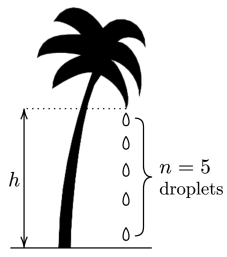
\includegraphics{images/Wet_Tree.png}
\end{figure}
\end{prbm}

\begin{proof}[Solution]
Consider the falling motion of a single droplet. Let the time taken for the droplet to reach the ground be $T$. From kinematics, we have:
\[ h = \frac{1}{2} gT^2 \]
Throughout the duration of its fall, an additional $n$ droplets must have fallen from the tree, such that the $n$-th additional droplet falls exactly when the initial droplet hits the ground. This condition is necessary to ensure that there are always $n$ droplets falling mid-air. Hence, $T$ must be related to $t$ by:
\[ T = nt \]
We can then solve for $h$:
\begin{align*}
h &= \frac{1}{2}g(nt)^2 \\
\Aboxed{h &\approx 120\:\unit{m}}
\end{align*}
\end{proof}
\pagebreak

\begin{prbm}[The Monkey and the Hunter Problem]
A student fires a dart at a stuff monkey held by an electromagnet a distance $h$ vertically above the dart gun and a distance $R$ horizontally away from the dart gun. The student aims directly at the monkey and fires, but as the student fires, the power of the electromagnet is turned off, causing the monkey to drop simultaneously. Will the dart hit the monkey?
\end{prbm}

\begin{figure}[H]
    \centering
    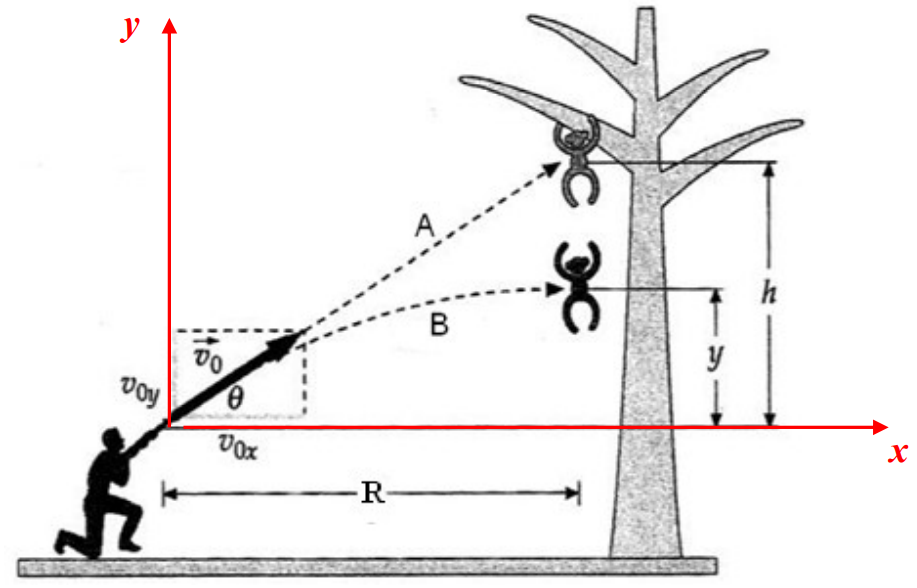
\includegraphics[width=12cm]{images/Monkey_hunter.png}
\end{figure}

\begin{solution}
It takes time $t$ the dart to travel a horizontal distance $R$:
\[ t=\frac{R}{v_0\cos\theta} \]

At time $t$,
\[ y_d=v_0\sin\theta t-\frac{1}{2}gt^2,\:y_m=h-\frac{1}{2}gt^2 \]

Difference in $y$-position at time $t$:
\begin{align*}
y_d-y_m 
&= \brac{v_0\sin\theta t - \frac{1}{2}gt^2} - \brac{h-\frac{1}{2}gt^2} \\
&= v_0\sin\theta t - h \\
&= v_0\sin\theta\frac{R}{v_0\cos\theta}-h \\
&= R\tan\theta - h \\
&= R\brac{\frac{h}{R}}-h = 0
\end{align*}
Therefore, the dart will hit the monkey.
\end{solution}
\pagebreak

\begin{prbm}
As the ball here rolls down the hill as shown in the figure below, describe the variation in its speed and acceleration.
\begin{figure}[H]
    \centering
    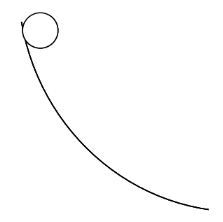
\includegraphics[width=5cm]{images/ball_roll.png}
\end{figure}
\end{prbm}

\begin{proof}[Answer]
Slope of the hill gets gentler as the ball rolls down, so \textbf{acceleration decreases}. 

Though acceleration decreases, it is always acting downwards, so \textbf{speed increases} due to the conversion of gravitational potential energy to kinetic energy (conservation of energy).
\end{proof}

\pagebreak
\section{Dynamics}
When drawing a \textbf{free body diagram}:
\begin{itemize}
	\item Draw all external forces acting only on the chosen system.
	\item Do not draw in the resultant force.
\end{itemize}

\subsection{Newton's Laws of Motion}
\begin{defn}{Newton's 1st Law of Motion}{}
A body at rest will remain at rest, a body in motion will remain in motion at constant velocity, \underline{in absence of external resultant force}. 
\end{defn} 

\begin{defn}{Newton's 2nd Law of Motion}{}
Rate of change of momentum is directly proportional to \underline{external} resultant force acting on it, and occurs in the direction of the external resultant force. 
\begin{equation} \sum \vb{F} = \dv{\vb{p}}{t} \end{equation}
(The constant of proportionality is found experimentally to be 1.)
\end{defn}

\begin{remark}
For questions, you will usually use the form $\displaystyle\sum\vb{F}=\frac{\Delta\vb{p}}{\Delta t}$.
\end{remark}

\begin{remark}
Using product rule, we have 
\[ \sum \vb{F}=\dv{\vb{p}}{t}=\dv{(m\vb{v})}{t}=m\dv{\vb{v}}{t}+\vb{v}\dv{m}{t} \]
Hence $\sum F = ma$ holds only when mass is constant.
\end{remark}

\begin{remark}
Resultant force and acceleration act in the same direction.
\end{remark}

\begin{defn}{Newton's 3rd Law of Motion}{}
When body A exerts a force on body B, body B exerts force of the \underline{same type}, \underline{equal in magnitude}, \underline{opposite in direction} on body A. 
\begin{equation} \vb{F}_{AB} = - \vb{F}_{BA} \end{equation}
\end{defn}

\begin{defn}{Inertia}{}
Reluctance of a body to change its state of rest or uniform motion in a straight line, due to mass. 
\end{defn} 
\begin{remark}
Mass is the property of a body which resists change in motion (inertia).
\end{remark}
\pagebreak

\subsection{Linear momentum and its conservation}
\begin{defn}{Linear momentum}{}
Product of a body's mass and velocity. 
\begin{equation}
\vb{p} = m\vb{v}
\end{equation}
\end{defn} 

\begin{defn}{Impulse}{}
Product of a constant force $F$ and the time interval $t$ for which the constant force acts. 
\begin{equation} 
\vb{J} = \int\vb{F}\dd{t} = \vb{F}_{\mathrm{avg}} \Delta t \end{equation}
\end{defn} 
Graphically, impulse is the area under a force-time graph. 

For collisions, the area under both graphs (representing impulse of force on each object by the other) must be the same, as linear momentum is conserved.

\begin{defn}{Impulse-Momentum Theorem}{}
The impulse applied to a body is equal to the body's change in momentum.
\begin{equation}
\vb{J} = \Delta\vb{p} = \vb{p}_f-\vb{p}_i
\end{equation}
\end{defn} 

\begin{defn}{Principle of Conservation of Momentum}{}
Total momentum of a \underline{system} of bodies is constant, provided \underline{no external resultant force} acts on the system.
\begin{equation}
\sum \vb{F} = 0 \implies \vb{J} = 0 \implies \vb{p}_i=\vb{p}_f
\end{equation}
\end{defn} 
\pagebreak

\subsection{Collisions}
\subsubsection{1D collision}
\textbf{Head-on collision}: contact forces between the two objects act radially along a line joining their centres of mass, with no component tangential to their circumference.

Types of collisions:
\begin{enumerate}
\item \textbf{Elastic} collision
\item \textbf{Inelastic} collision
\item \textbf{Perfectly inelastic} collision (coalescence)
\item \textbf{Super elastic} collision
\end{enumerate}

Problem solving:
\begin{itemize}
\item \textbf{Linear momentum} is always conserved for every type of collision (except super elastic collisions). \[ m_1 u_1 + m_2 u_2 = m_1 v_1 + m_2 v_2 \]

\item \textbf{Kinetic energy} is conserved for elastic collisions, from which we can derive: relative speed of approach = relative speed of separation (r.s.a. = r.s.s.) \[ u_1-u_2 = v_2-v_1 \] 
 
Kinetic energy is not conserved for inelastic collisions, is lost to surroundings, hence relative speed of approach $>$ relative speed of separation (r.s.a $>$ r.s.s.) \[ u_1-u_2 > v_2-v_1 \]

Kinetic energy is not conserved for super elastic collisions, is gained due to stored forms of energy (potential energy) e.g. bullet shot at a stationary hand grenade and a hand grenade explodes, where the additional energy comes from chemical energy of explosives stored in the grenade.
\end{itemize}

\subsubsection{2D collision}
\textbf{Oblique collision}: 
If an object obliquely collides with another stationary object of equal mass, they travel off at an angle of 90° relative to one another (for elastic collision).
\pagebreak

\subsection{Problems}
\begin{prbm}[Stacked ball drop]
Two balls are dropped to the floor, with the lighter ball atop the heavier one. The balls collide approximately elastically with each other and with the floor. The observation is the small ball flies up to a height higher than it was dropped.
\end{prbm}
\begin{solution} \ {\\}
\begin{figure}[H]
    \centering
    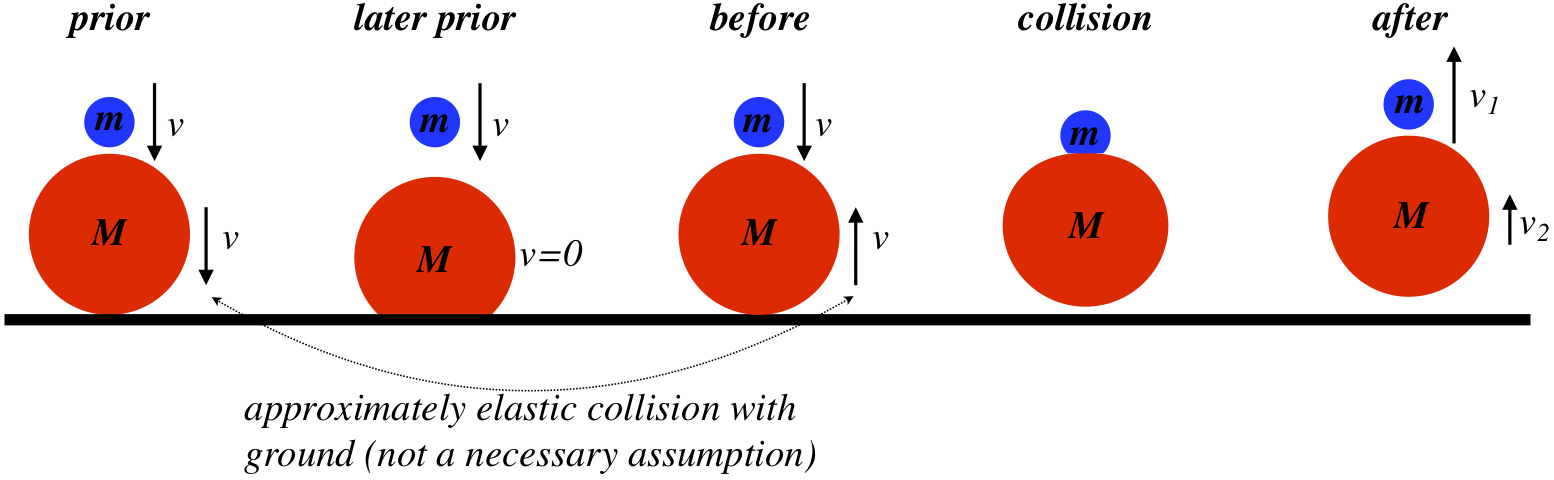
\includegraphics[width=15cm]{images/Stacked_balls.png}
\end{figure}

Conservation of momentum gives us 
\[ Mv - mv = mv_1 + Mv_2 \]
Conservation of kinetic energy gives us 
\[ \frac{1}{2}mv^2 + \frac{1}{2}Mv^2 = \frac{1}{2}m{v_1}^2 + \frac{1}{2}M{v_2}^2 \]

We can now solve for $v_1$ and $v_2$ in terms of $v$, which we can determine from the height that the balls are dropped from.
\[ v_1=\brac{\frac{3M-m}{M+m}}v \]
\[ v_2=\brac{\frac{M-3m}{M+m}}v \]

We see that the small ball must rise to a height greater than that from which it was dropped, because the fraction in front of $v$ is always greater than 1.
\end{solution}
\pagebreak

\begin{prbm}
A flatcar of mass $m$ moves towards the right from rest due to a constant horizontal force $F$. At the same time, sand spills on the flatcar from a stationary hopper at a constant rate of $\mu\:\unit{kg.s^{-1}}$. 

\begin{figure}[H]
    \centering
    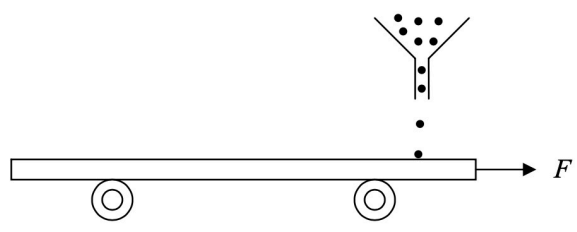
\includegraphics[width=10cm]{images/Sand_car.png}
\end{figure}

What is the dependence of the velocity $v$ of the flatcar with respect to time $t$, assuming that friction is negligibly small?
\end{prbm}

\begin{solution}
Recall that force is the rate of change of momentum. 
\[ F=\dv{p}{t} \implies \Delta p=F\Delta t \]
The momentum of the flatcar due to from the additional mass of the sand which is $\mu t$, as well as from the increase in velocity $v$. 

At time $t = 0$, $p = 0$. At time $t = t$, the momentum is 
\[ p=(m+\mu t)v=Ft \]

Hence we get \[ \boxed{v=\frac{Ft}{m+\mu t}} \]
\end{solution}
\pagebreak
\section{Forces}
\subsection{Types of force}
\begin{defn}{Hooke's Law}{}
Force is directly proportional to extension of a spring, provided that the \underline{elastic limit} has not been exceeded.
\[ F \propto x \]
\begin{equation} F = kx \end{equation}
where $k$ is the \textbf{spring constant}.
\end{defn}

\begin{itemize}
\item For springs in \textbf{parallel}, 
\begin{equation} k_{\text{eff}} = \sum_{i} k_i \end{equation}
\item For springs in \textbf{series},
\begin{equation} \frac{1}{k_{\text{eff}}} = \sum_{i} \frac{1}{k_i} \end{equation}
\end{itemize}

\textbf{Elastic potential energy} stored in an object when it undergoes deformation (when a spring is extended or compressed).
\begin{equation} U = \frac{1}{2}Fx = \frac{1}{2}kx^2 \end{equation}
Graphically, elastic potential energy is the area under a force-extension graph.
\[ W = \int F \dd{x} \]

\subsection{Upthrust}
\textbf{Pressure} $P$ of a liquid column is given by 
\begin{equation}
P=\rho gh
\end{equation}

\deriv{See Appendix for the derivation.}

\begin{defn}{Upthrust $U$}{}
Vertical upward force exerted by the surrounding fluid when a body is submerged, fully or partially, in a fluid.
\end{defn} 

\begin{remark}
Origin of upthrust: Upthrust is the \underline{resultant} force due to the difference in pressure exerted by fluid at the top and bottom surfaces of the body.
\end{remark}

\begin{defn}{Archimedes' Principle}{}
Upthrust is \underline{equal in magnitude}, \underline{opposite in direction} to the weight of fluid displaced by the body.
\begin{equation} 
    U = W_{\text{displaced}} = \rho_{\text{fluid}}\, V_{\text{displaced}}\,g 
\end{equation}
\end{defn}

\deriv{See Appendix for the derivation.}

For an object floating in equilibrium, upthrust is equal in magnitude, opposite in direction to weight of the object.
\begin{equation} U = W_{\mathrm{object}} \end{equation}

\subsection{Centre of gravity}
\begin{defn}{Centre of gravity}{}
A single point where the entire weight of the object may be taken as acting at.
\end{defn} 

\subsection{Turning effects of forces}
\begin{defn}{Moment of a force}{}
Product of magnitude of the force and perpendicular distance of the \emph{line of action} of the force from the pivot point.
\begin{equation} M = F \times \perp d \end{equation}
\end{defn}

\begin{defn}{Couple}{}
A pair of forces of \underline{equal magnitude} but acting in \underline{opposite directions} whose lines of action are \underline{parallel but separate}.
\end{defn} 

\begin{remark}
A couple is a pair of forces which tends to produce \emph{rotation} only.
\end{remark}

\begin{defn}{Torque of a couple}{}
Product of one of the forces and the perpendicular distance between the forces.
\begin{equation} \tau = F \times \perp d \end{equation}
\end{defn}

\begin{defn}{Principle of Moments}{}
When a system is in equilibrium, sum of clockwise moments \underline{about any axis} must be equal to sum of anticlockwise moments \underline{about the same axis}.
\begin{equation} \sum \text{ clockwise moments} = \sum \text{ anticlockwise moments} \end{equation}
\end{defn} 
\pagebreak

\subsection{Equilibrium of forces}
A system is in equilibrium when there is 
\begin{itemize}
\item no resultant force, and
\item no resultant torque
\end{itemize}

\begin{defn}{Translational equilibrium}{}
Net force is zero \underline{in any direction}.
\[ \sum \va{F} = 0 \]
\end{defn} 

\begin{defn}{Rotational equilibrium}{}
Net torque is zero \underline{about any axis of rotation}. 
\[ \sum \va{\tau} = 0 \]
\end{defn}

For multiple non-parallel forces, this is illustrated by: 
\begin{itemize}
\item Forces form a \textbf{closed vector polygon}.
\item Lines of actions of forces \textbf{intersect at one point}, so that there is no resultant moment about their point of intersection.
\end{itemize}
\pagebreak

\subsection{Problems}
\begin{prbm}
Explain why the upthrust acting on a human body when in air is normally ignored.
\end{prbm}
\begin{proof}[Answer]
The average person weighs about 600 \unit{N}. Upthrust by air is about 1 \unit{N}, less than 0.2\% of the weight of the person.
\end{proof}

\begin{prbm}
Why can a lump of plasticine moulded into the shape of a bowl float in water?
\end{prbm}
\begin{proof}[Answer]
Bowl is able to displace a greater volume of water.

If the plasticine floats, 
\[ W = U \]
\[ \rho_{\mathrm{plasticine}} g V_{\mathrm{plasticine}} = p_{\mathrm{water}} g V_{\mathrm{water\:displaced}} \]

Since $p_{\mathrm{plasticine}} > \rho_{\mathrm{water}}$, in order for the plasticine to float, $V_{\mathrm{water\:displaced}} > V_{\mathrm{plasticine}}$.

Hence plasticine must be able to displace a larger volume of water than its own volume.
\end{proof}
\pagebreak

\begin{prbm}
A rope is connected to a vertical wall at one end, and a horizontal external force $F = 15.0$ N pulls on the other end. The rope is in equilibrium and makes an angle $\theta = 25.0\degree$ with the wall. What is the weight $W$ of the rope? 

\textit{Leave your answer to $3$ significant figures in units of \emph{N}}.

\begin{figure}[H]
    \centering
    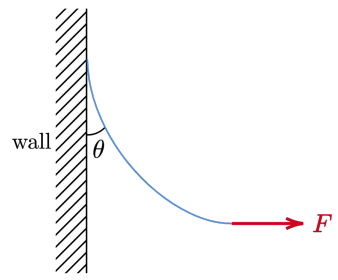
\includegraphics{images/Mysterious_Rope.png}
\end{figure}
\end{prbm}

\begin{proof}[Solution]
Since the rope makes an angle $\theta$ with the wall, and the tension in the rope acts along the rope, we can write the following force balance equations for the horizontal and vertical axes respectively:
\[ T \sin \theta = F \]
\[ T \cos \theta = W \]
Hence solving for $W$,
\begin{align*}
W &= \frac{F \cos \theta}{\sin \theta} \\
W &= F \cot \theta \\
\Aboxed{W &\approx 32.2\:\unit{N}}
\end{align*}
\end{proof}
\pagebreak

\begin{prbm}[Sailor capstan]
A capstan is a device used aboard ships in order to control a rope that is under great tension. The rope is wrapped around a fixed drum of radius $R$, usually for several turns. The load on the rope pulls it with a force $T_A$, and the sailor holds the other end of the rope with a much smaller force $T_B$. The coefficient of static friction between the rope and the drum is $\mu_s$. The sailor is holding the rope so that it is just about to slip.

\begin{figure}[H]
    \centering
    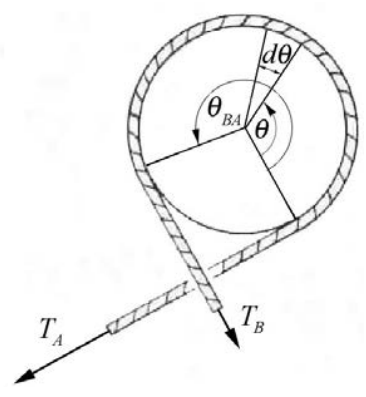
\includegraphics[width=6cm]{images/Capstan.png}
\end{figure}

Show that \[ T_B = T_Ae^{-\mu_s \theta_{BA}}\]
where $\theta_{BA}$ is the angle subtended by the rope on the drum. 
\end{prbm}

\begin{proof}[Solution]
Analysing forces on a small slice of rope of arc length $R\Delta\theta$:

\begin{figure}[H]
    \centering
    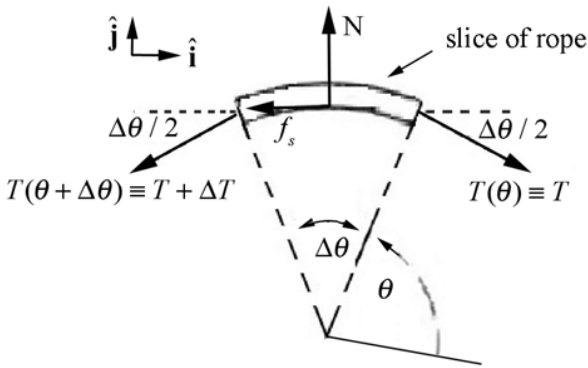
\includegraphics[width=8cm]{images/Capstan_1.png}
\end{figure}

In the horizontal direction,
\[ T\cos\frac{\Delta\theta}{2} - \brac{T+\Delta T}\cos\frac{\Delta\theta}{2} - f_s = 0 \]
In the vertical direction,
\[ N - T\sin\frac{\Delta\theta}{2} - \brac{T+\Delta T}\sin\frac{\Delta\theta}{2} = 0 \]

Solving the two equations simultaneously gives us 
\[ \frac{\Delta T}{\Delta \theta} = \mu_s T \]
As $\Delta \theta \to 0$, 
\[ \dv{T}{\theta} = -\mu_s T \]
Solving the differential equation,
\begin{align*}
\int_{T_A}^{T_B} \frac{1}{T} \dd{T} 
&= -\mu_s \int_{\theta_A}^{\theta_B} \dd{\theta} \\
\ln \frac{T_B}{T_A} &= -\mu_s\brac{\theta_B-\theta_A} \\
\Aboxed{T_B &= T_A e^{-\mu_s \theta_{BA}}}
\end{align*}

The exponential dependence suggests that the coefficient $e^{-\mu_s \theta_{BA}}$ becomes very small when $\theta_{BA}$ increases. Note that for $x$ turns of the rope, $\theta_{BA}=2\pi x$ radians.
\end{proof}
\pagebreak

\begin{prbm}[Yoyo problem]

\end{prbm}

\begin{proof}[Solution]

\end{proof}
\pagebreak

\begin{prbm}
What is the minimum force $F$ that must be applied to cause the cylinder to barely lift up off of the bottom step and rotate up around the corner of the next one? Assume that the cylinder does not slip on the corner of the next step.
\end{prbm}

\begin{figure}[H]
    \centering
    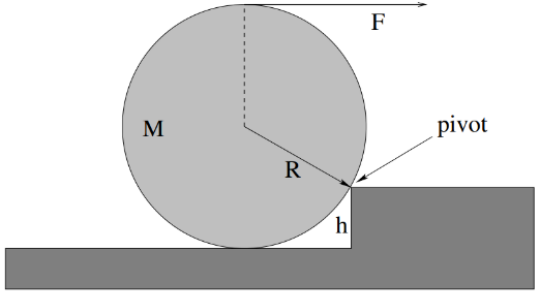
\includegraphics[width=10cm]{images/Cylinder_moment.png}
\end{figure}

\begin{proof}[Solution]
Computing the torques of $F$ and $Mg$ gives us 
\[ \boxed{F=\frac{Mg\sqrt{R^2-(R-h)^2}}{2R-h}} \]
\end{proof}

\pagebreak
\section{Work, Energy and Power}
\subsection{Work}
\begin{defn}{Work done (by constant force)}{}
Product of the force and displacement \underline{in the direction of the force}.
\begin{equation}
W=Fs\cos\theta
\end{equation}
In vector form, this is given by
\[ W=\vb{F}\cdot\vb{s} \]
\end{defn} 

\begin{itemize}
\item Work done by a \textbf{variable force} is given by
\begin{equation}
W=\int\vb{F}\dd{\vb{s}}
\end{equation}
Graphically, work done is area under force-displacement graph.

\item Work done to deform (stretch/compress) a material is stored as elastic potential energy in the material.
\begin{equation}
    U = \frac{1}{2}Fx = \frac{1}{2}kx^2
\end{equation}

\item Work done by a \textbf{gas} which is expanding against a constant external pressure: 
\begin{equation}
W = p \Delta V
\end{equation}

Graphically, work done is the area under a pressure-volume graph.
\[ W = \int p \dd{V} \]
\end{itemize}
\pagebreak

\subsection{Energy conversion and conservation}
\begin{defn}{Principle of Conservation of Energy}{}
Energy can neither be created nor destroyed, but can be transformed from one form to another, and transferred from one body to another. Total energy in a closed system is always constant.
 \begin{equation}
(E_k+E_p)_i + W = (E_k+E_p)_f
\end{equation}
\begin{remark}
Work done by dissipative forces is \emph{negative} as the forces act in opposite direction to displacement.
\end{remark}
\end{defn}

\textbf{Gravitational potential energy} is energy stored due to height raised.
\begin{equation}
\mathrm{GPE} = mgh
\end{equation}

\deriv{See Appendix for the derivation.}

\textbf{Kinetic energy} is energy possessed by an object due to motion.
\begin{equation} 
\mathrm{KE} = \frac{1}{2}mv^2 = \frac{p^2}{2m} 
\end{equation}

\deriv{See Appendix for the derivation.}

\textbf{Elastic potential energy} is energy stored in an object when it is deformed.
\begin{equation}
\mathrm{EPE} = \frac{1}{2} Fx = \frac{1}{2} k x^2 
\end{equation}

\begin{defn}{Work-Energy Theorem}{}
Net work done by a force on a body is equal to the change in kinetic energy of the body.
\begin{equation} W = \Delta \mathrm{KE} \end{equation}
\end{defn} 

The relationship between conservative force $F$ and potential energy $U$ is
\begin{equation}
\vb{F}=-\dv{U}{\vb{x}}
\end{equation}
\begin{remark}
A conservative force is one where work done by the force is independent of its path.
\end{remark}
\pagebreak

\subsection{Power}
\begin{defn}{Power}{}
Rate at which work is done; rate at which energy is transferred.
\begin{equation}
P = \dv{W}{t}
\end{equation}
\end{defn}

\vocab{Instantaneous power} $P$ when a constant force $F$ acts on an object with velocity $v$ is given by
\begin{equation} P = Fv \end{equation}
\begin{remark}
This means power is the product of a force and velocity in the direction of the force.
\end{remark}

\vocab{Average power} $P_{\mathrm{avg}}$ when a constant force $F$ acts on an object with average velocity $v_{\mathrm{avg}}$ is given by
\begin{equation} P_{\mathrm{avg}} =  F v_{\mathrm{avg}} \end{equation}

\subsection{Efficiency}
\vocab{Efficiency} $\eta$ is given by
\begin{equation} \eta = \frac{\mathrm{useful\:power/energy\:output}}{\mathrm{total\:power/energy\:input}} \times 100\% \end{equation}
\pagebreak

\subsection*{Problems}
\begin{prbm}
A hydroelectric dam has a water height of $50\:\unit{m}$ (as measured from the bottom of the dam where water is let out). What is the rate at which water is let out to produce $50\:\unit{MW}$ of electrical power? You should assume an energy conversion efficiency of the dam (from mechanical to electrical) to be $30\%$, and the density of water as $997\:\unit{kg\,m^{-3}}$.

Assume that the dam is large enough so that the water height does not substantially change during power generation.
\end{prbm}

\begin{proof}[Solution]
By conservation of energy, the kinetic energy of water that leaves the bottom of the dam is equal to gravitational potential energy at the top of the dam.

Power generated is (efficiency) × (rate of flow) × (density) × g × (50 metres). Equating this to $50\:\unit{MW}$ produces a rate of flow of $341\:\unit{m^3\,s^{-1}}$.
\end{proof}
\pagebreak
\section{Circular motion}
\subsection{Uniform circular motion}
\vocab{Uniform circular motion} is a type of motion in which an object moves at a \textit{constant speed} in a circular path.

\begin{defn}{Radian}{}
Unit of angular measure, defined as the angle subtended at the centre of a circle by an arc of a length equal to the radius of the circle.
\end{defn}

\vocab{Angular displacement} $\theta$ refers to the angle in radians through which a point is rotated.
\begin{equation} \theta = \frac{s}{r} \end{equation}

\begin{figure}[H]
    \centering
    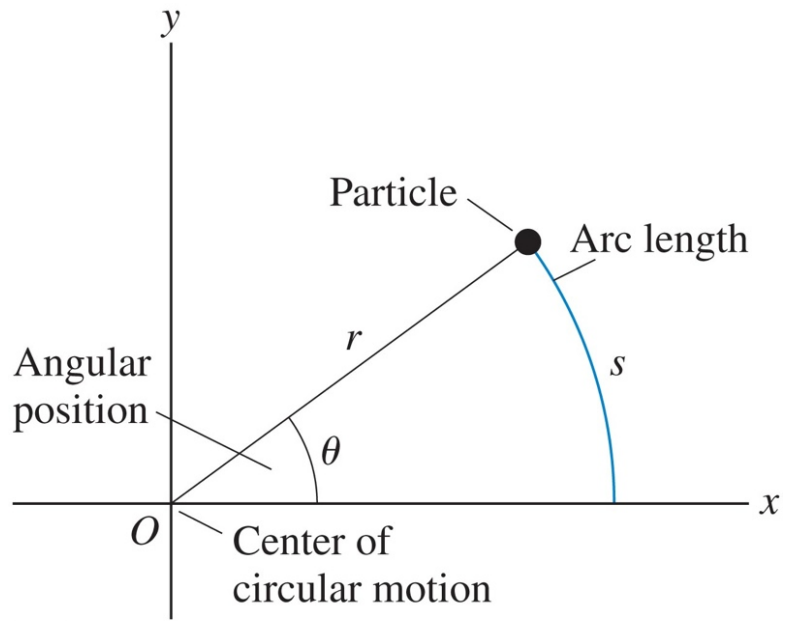
\includegraphics[width=8cm]{images/Angular_displacement.png}
\end{figure}

\vocab{Angular velocity} $\omega$ refers to rate of change of angular displacement.
\begin{equation} \omega = \dv{\theta}{t} \end{equation}

Relating angular velocity to period $T$ and frequency $f$, 
\begin{equation} \omega = \frac{2\pi}{T} = 2\pi f \end{equation}

\vocab{Linear velocity} $v$ is given by 
\begin{equation} v = r\omega \end{equation}

\vocab{Centripetal acceleration} $a$ is given by
\begin{equation} a = \frac{v^2}{r} = r\omega^2 \end{equation}

\vocab{Centripetal force} $F_c$ is given by
\begin{equation} F_c = \frac{mv^2}{r} = mr\omega^2 \end{equation}
\begin{remark}
Centripetal force is a \textbf{resultant force}; it can be provided by gravitational force, friction force, normal force, etc. 
\end{remark}

\begin{tcolorbox}
\textbf{Why does a resultant force exist in a uniform circular motion?}

Velocity changes due to change in direction, hence the object undergoes acceleration. By Newton's 2nd Law, a resultant force acts on the object. 

Since the force does not change the speed of the object, it does no work to accelerate the object, thus centripetal force acts \underline{perpendicularly} to motion, towards the \underline{centre} of the circle.
\end{tcolorbox}

\subsection{Non-uniform circular motion}
Consider an object rotating vertically in a circle of radius $r$.
\begin{figure}[H]
	\centering
	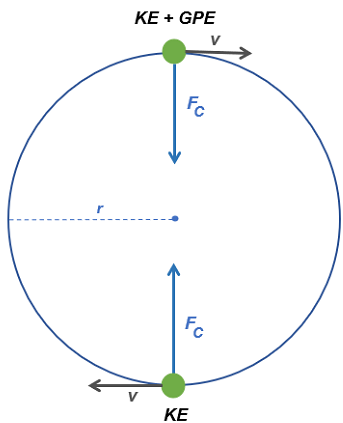
\includegraphics[width=6cm]{Vertical_circular_motion}
\end{figure}

Tension in the spring reaches maximum at the bottom and minimum at the top.

At the top, if the string is just taut, $mg$ provides centripetal force completely, $T=0 \unit{N}$.
\begin{align*}
mg &= \frac{m{v_{\text{top}}}^2}{r}\\
v_{\text{top}} &= \sqrt{gr}
\end{align*}
At the bottom, by conservation of mechanical energy,
\begin{align*}
\frac{1}{2} m{v_{\text{bottom}}}^2 &= mg(2r) + \frac{1}{2} m{v_{\text{top}}}^2\\
v_{\text{bottom}} &= \sqrt{5gr}
\end{align*}
\pagebreak

\subsection*{Problems}
2014 P1 Q11, Q12, 2015 P1 Q10, 2016 P1 Q13, 2019 P1 Q10, 
2013 P2 Q3 (pg 7(7)) 
\pagebreak
\section{Gravitational Field}
\subsection{Gravitational force}
\begin{defn}{Newton's Law of Gravitation}{}
Gravitational force of attraction between two \underline{point masses} is directly proportional to the product of their masses and inversely proportional to the square of \underline{separation} between their centres.
\begin{equation} \va{F}_g = -\frac{GMm}{r^2}\hat{r} \end{equation}
where gravitational constant $G = 6.67 \times 10^{-11}$ \unit{kg^{-1}.m^3.s^{-2}}
\end{defn} 

\begin{itemize}
    \item The sign is negative due to the attractive nature of gravitational force. (The negative sign is ignored when only the magnitude of the force is required.)
    \item The gravitational forces between two masses are an action-reaction pair; they are equal in magnitude, opposite in direction, and act along the line joining the two point masses.
    \item \textbf{Point masses} have their masses concentrated at one point. Two objects can be considered point masses when they are placed \emph{sufficiently far apart} such that their \emph{dimensions} become negligible compared to the \emph{distance} separating them.
\end{itemize}

\subsection{Gravitational field}
\begin{defn}{Gravitational field}{}
\underline{Region of space} where a mass experiences gravitational force.
\end{defn}

\begin{itemize}
    \item A field of force is a region of space where they may be a \emph{non-contact} force acting on an object placed in that field due to interaction between the field's property and the object's property.
    \item Field lines are used to indicate the direction of a field of force. Density of field lines corresponds to strength of field. (Field lines never touch or cross.)
    \item Gravitational field around Earth is non-uniform (field strength is stronger near Earth, weaker further away from Earth). Field lines are drawn radially pointing towards the centre of Earth.
    \item Gravitational field near Earth's surface is uniform (field strength is the same at all points). Field lines are drawn parallel to each other and of equal spacing.
\end{itemize}

\begin{defn}{Gravitational field strength $g$}{}
Gravitational force per unit mass exerted on a \emph{small test mass} placed at that point.
\begin{equation}
\va{g} = \frac{\va{F}}{m} = -\frac{GM}{r^2}\hat{r} 
\end{equation}
This means that the gravitational field is a inverse square field.
\end{defn} 

\deriv{See Appendix for the derivation.}

This expression refers to the gravitational field created by mass $M$ in its surrounding region of space, where a gravitational force acts on mass $m$.

\begin{itemize}
\item The sign is negative due to the attractive nature of gravitational force acting on a mass in the field. (The negative sign is ignored when only the magnitude is required.)
\item A \textbf{neutral point} refers to the point at which the resultant gravitational field due to surrounding masses is zero.
\begin{figure}[H]
    \centering
    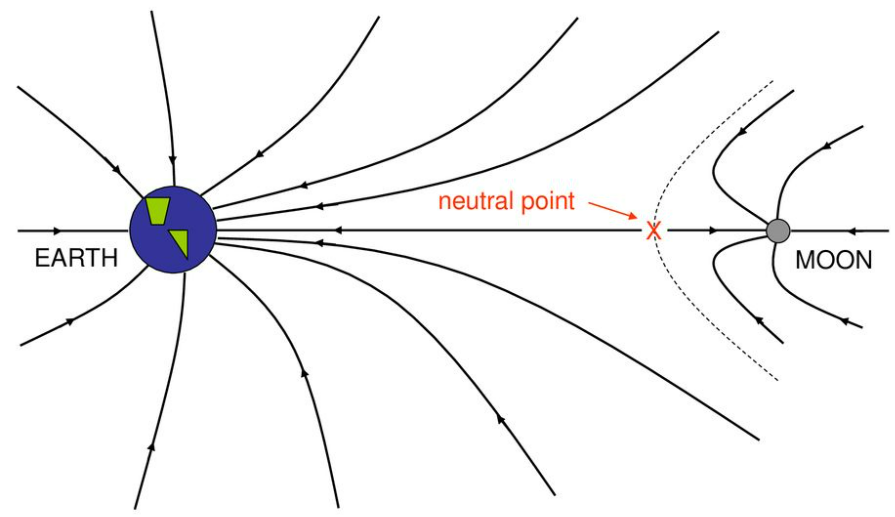
\includegraphics[width=12cm]{images/Neutral_point.png}
    \end{figure}
\end{itemize}

Near the surface of Earth, $g$ can be approximated to have a constant value of $\mathbf{9.81}$ \unit{N.kg^{-1}}, equal to the acceleration of free fall.
\pagebreak

\subsection{Gravitational potential energy}
\begin{defn}{Gravitational potential energy $U$}{}
\underline{Work done} by an \underline{external force} in bringing a \underline{small test mass} from infinity to that point.
\begin{equation} U = -\frac{GMm}{r} \end{equation}
\end{defn}

\begin{itemize}
\item Note that the negative sign cannot be omitted.
\item Maximum $U$ is defined to be 0 at $r=\infty$, hence $U$ is negative.
\item Work done is negative as force and displacement act in opposite directions, hence $U$ is negative.
\end{itemize}

\begin{defn}{Gravitational potential $\phi$}{}
Work done per unit mass by an external force in bringing a small test mass from infinity to that point.
\begin{equation} \phi = \frac{U}{m} = -\frac{GM}{r} \end{equation}
\end{defn}

\begin{itemize}
\item Note that the negative sign cannot be omitted.
\item For the same reasons as above, $\phi$ is negative.
\end{itemize}
\pagebreak

\subsection{Relationship summary}
\begin{figure}[H]
    \centering
    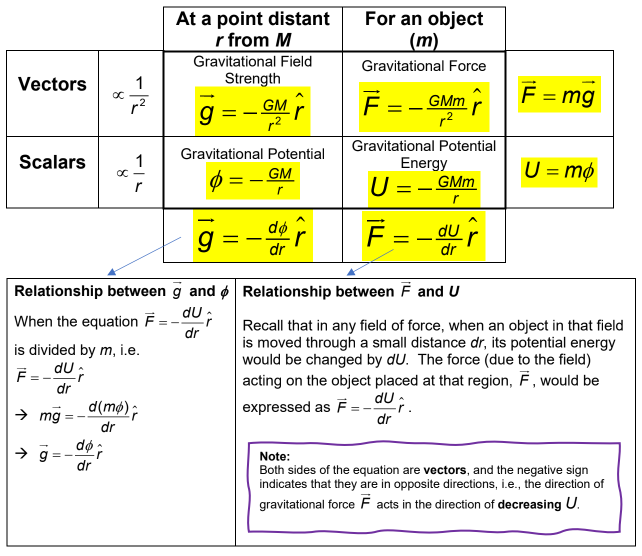
\includegraphics[width=\textwidth]{images/g_field_relationship_summary.png}
\end{figure}
\pagebreak

\subsection{Graphs}
\subsubsection{Force-distance}
Force-distance graph (point mass):
\begin{figure}[H]
\centering
      \begin{tikzpicture}[scale=.4] 
        \draw[->] (-10, 0) -- (10, 0) node[right] {$r$};
        \draw[->] (0, -10) -- (0, 5) node[above] {$\va{F}_g$};
        \draw[color=red, domain=-10:-1,samples=200] plot[id=x1] function{10/x};
        \draw[color=red, domain=1:10,samples=200] plot[id=x2] function{-10/x};
    \end{tikzpicture}
\end{figure}

Force-distance graph (planet):
\begin{figure}[H]
\centering
      \begin{tikzpicture}[scale=.4] 
        \draw[->] (-10, 0) -- (10, 0) node[right] {$r$};
        \draw[->] (0, -10) -- (0, 5) node[above] {$\va{F}_g$};
        \draw[color=red, domain=-10:-2,samples=200] plot[id=x1] function{10/x};
        \draw[color=red, domain=2:10,samples=200] plot[id=x2] function{-10/x};
        \draw[color=red,domain=0:2,samples=200] plot[id=x3] function{-2.5*x};
        \draw[color=red,domain=-2:0,samples=200] plot[id=x3] function{2.5*x};
        \draw[color=black] (0,0) circle (2.0);
    \end{tikzpicture}
\end{figure}
\pagebreak

\subsubsection{Field-distance}
Field-distance graph (point mass)
\begin{figure}[H]
\centering
    \begin{tikzpicture}
    \begin{axis}%
    [axis lines=middle,
     enlargelimits={abs=0.2},
     xlabel = $r$,
     ylabel = $\va{g}$,
     ticks=none
    ]
   \addplot[domain=1:10,samples=200,smooth,red] {-1/x};
   \addplot[domain=-10:-1,samples=200,smooth,red] {-1/x};
    \end{axis}
    \end{tikzpicture}
\end{figure}

Field-distance graph (planet)
\begin{figure}[H]
\centering
    \begin{tikzpicture}
    \begin{axis}%
    [axis lines=middle,
     enlargelimits={abs=0.2},
     xlabel = $r$,
     ylabel = $\va{g}$,
     ticks=none
    ]
   \addplot[domain=1:10,samples=200,smooth,red] {-10/x};
   \addplot[domain=-10:-1,samples=200,smooth,red] {-10/x};
   \draw (axis cs:0,0) circle [radius=1];
   \addplot[mark=none, black,thick, dotted] coordinates {(-1,10) (-1,0)};
   \addplot[mark=none, black,thick, dotted] coordinates {(1,-10) (1,0)};
   \addplot[mark=none, red,thick] coordinates {(-1,10) (1,-10)};
    \end{axis}
    \end{tikzpicture}
\end{figure}

Field-distance graph between two masses
\begin{figure}[H]
\centering
\begin{tikzpicture}
  \begin{axis}%
    [axis lines=middle,
     enlargelimits={abs=0.2},
     xlabel = $r$,
     ylabel = $\va{g}$,
     ticks=none
    ]
   \addplot[domain=0:5,samples=50,smooth,red] {-1/x + 0.2};
%   \addplot[domain=5:9.5] {-1/(x-10) - 0.2}
  \end{axis}
\end{tikzpicture}
\end{figure}
\pagebreak

\subsubsection{Energy-distance}
Energy-distance graph (point mass)
\begin{figure}[H]
\centering
    \begin{tikzpicture}
    \begin{axis}%
    [axis lines=middle,
     enlargelimits={abs=0.2},
     xlabel = $r$,
     ylabel = $U$,
     ymax = 0,
     ticks=none
    ]
   \addplot[domain=1:10,samples=200,smooth,red] {-1/x};
   \addplot[domain=-10:-1,samples=200,smooth,red] {1/x};
    \end{axis}
    \end{tikzpicture}
\end{figure}

Energy-distance graph (planet)
\begin{figure}[H]
\centering
    \begin{tikzpicture}
    \begin{axis}%
    [axis lines=middle,
     enlargelimits={abs=0.2},
     xlabel = $r$,
     ylabel = $U$,
     ymax = 2,
     ticks=none
    ]
   \addplot[domain=1:7,samples=200,smooth,red] {-10/x};
   \addplot[domain=-7:-1,samples=200,smooth,red] {10/x};
   \draw (axis cs:0,0) circle [radius=1];
   \addplot[mark=none, black,thick, dotted] coordinates {(1,-10) (1,0)};
   \addplot[mark=none, black,thick, dotted] coordinates {(-1,-10) (-1,0)};
    \end{axis}
    \end{tikzpicture}
\end{figure}

Energy-distance of satellite (GPE, KE, TE)
\begin{figure}[H]
\centering
\begin{tikzpicture}
    \begin{axis}%
    [axis lines=middle,
     enlargelimits={abs=0.2},
     xlabel = $r$,
     ylabel = $U$,
     xmin = -2,
     ticks=none
    ]
   \addplot[domain=1:10,samples=200,smooth,red] {-10/x};
   \addplot[domain=1:10,samples=200,smooth,blue] {5/x};
   \addplot[domain=1:10,samples=200,smooth,darkgray] {-5/x};
    \end{axis}
\end{tikzpicture}
\end{figure}
\pagebreak

\subsubsection{Potential-distance}
Potential-distance graph (point mass)
\begin{figure}[H]
\centering
    \begin{tikzpicture}
    \begin{axis}%
    [axis lines=middle,
     enlargelimits={abs=0.2},
     xlabel = $r$,
     ylabel = $\phi$,
     ymax = 2,
     xmin = -2,
     ticks=none
    ]
   \addplot[domain=1:12,samples=200,smooth,red] {-10/x};
    \end{axis}
    \end{tikzpicture}
\end{figure}

Potential-distance graph (planet)
\begin{figure}[H]
\centering
    \begin{tikzpicture}
    \begin{axis}%
    [axis lines=middle,
     enlargelimits={abs=0.2},
     xlabel = $r$,
     ylabel = $\phi$,
     ymax = 2,
     xmin = -2,
     ticks=none
    ]
   \addplot[domain=1:12,samples=200,smooth,red] {-10/x};
   \draw (axis cs:0,0) circle [radius=1];
   \addplot[mark=none, black,thick, dotted] coordinates {(1,-10) (1,0)};
    \end{axis}
    \end{tikzpicture}
\end{figure}

Potential-distance graph between two masses
\begin{figure}[H]
\centering
\begin{tikzpicture}
    \begin{axis}%
    [axis lines=middle,
     enlargelimits={abs=0.2},
     xlabel = $r$,
     ylabel = $\phi$,
     ticks=none
    ]
    
    \end{axis}
\end{tikzpicture}
\end{figure}
\pagebreak

\subsection{Applications}
\subsubsection{Orbit velocity}
For a satellite of mass $m$ orbiting a planet of mass $M$ at a certain orbital velocity, \textbf{gravitational force provides centripetal force}.
\begin{align*}
F_g &= F_c \\
\frac{GMm}{r^2} &= \frac{mv^2}{r}
\end{align*}
\[ \boxed{v = \sqrt{\frac{GM}{r}}} \]

\subsubsection{Kinetic energy}
For a satellite in orbit, \textbf{gravitational force provides centripetal force}.
\[ \frac{GMm}{r^2}=\frac{mv^2}{r} \implies mv^2=\frac{GMm}{r} \implies \frac{1}{2}mv^2=\frac{GMm}{2r} \]
\[ \boxed{\mathrm{KE}=\frac{GMm}{2r}} \]

\subsubsection{Kepler's Third Law}
\vocab{Kepler's Third Law} states that the ratio of the square of a body's orbital period to the cube of the axis of orbit is the same for all objects orbiting the same primary.
\begin{equation} T^2 \propto r^3 \end{equation}

\begin{proof}[Derivation]
\textbf{Gravitational force provides centripetal force.}
\[ \frac{GMm}{r^2} = mr \omega ^2 = mr\left(\frac{2 \pi}{T}\right)^2 \]
Making period $T$ the subject, 
\[ T^2 = \frac{4 \pi ^2}{GM} r^3 \implies \boxed{T^2 \propto r^3} \]
\end{proof}

\subsubsection{Escape speed}
\textbf{Escape speed} refers to the \underline{minimum} speed required to escape the effect of a gravitational field.

By conservation of energy,
\[ \text{KE}_i + U_i = \text{KE}_f + U_f \]
At infinity, $U_f = 0$ (by definition of gravitational potential energy) and $\text{KE}=0$ (by definition of escape speed).
\[ \frac{1}{2} mv^2 + \brac{-\frac{GMm}{r}} = 0 \]
Making $v$ the subject,
\[ \boxed{v = \sqrt{\frac{2GM}{r}}} \]

\subsubsection{Geostationary satellite}
\begin{defn}{Geostationary satellite}{}
A satellite that \underline{appears stationary} when observed from a \underline{fixed location} from Earth.
\end{defn}

Characteristics:
\begin{enumerate}
\item Orbital period is the same as the rotational period of Earth about its axis, i.e. $T = 24$ \unit{hr}.
\item Moves in the same direction as the rotation of Earth about its own axis, i.e. from west to east.
\item Vertically above the equator, so that its axis of rotation is the same as the Earth.
    \begin{itemize}
    \item Gravitational force by Earth is the resultant force that provides centripetal force for the satellite. 
    \item Gravitational force is directed towards centre of \underline{Earth}, centripetal force is directed towards centre of \underline{orbit},
    \item so centre of orbit must be centre of Earth.
    \end{itemize}
\end{enumerate}
\pagebreak
\subsubsection{Binary star system}
In a binary star system, two stars rotate about their \emph{common} centre of mass.
\begin{figure}[H]
	\centering
	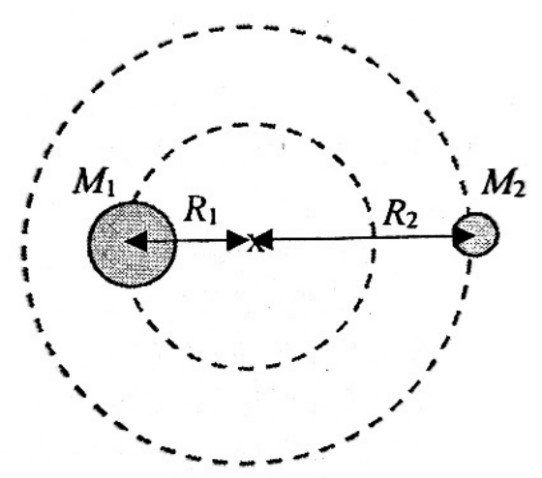
\includegraphics[width=6cm]{Binary_stars}
\end{figure}
For mass $M_1$, gravitational force provides centripetal force for orbit.
\begin{align*}
F_g &= F_c \\
\frac{GM_1M_2}{(R_1+R_2)^2} &= M_1R_1\omega^2 \\
\frac{GM_2}{(R_1+R_2)^2} &= R_1\omega^2
\end{align*}
For mass $M_2$, gravitational force provides centripetal force for orbit.
\begin{align*}
F_g &= F_c \\
\frac{GM_1M_2}{(R_1+R_2)^2} &= M_2R_2\omega^2 \\
\frac{GM_1}{(R_1+R_2)^2} &= R_2\omega^2
\end{align*}
Adding the two equations gives us the period of rotation:
\[ \frac{G(M_1+M_2)}{(R_1+R_2)^2} = (R_1+R_2)\brac{\frac{2\pi}{T}}^2 \]
\[ \boxed{T = \sqrt{\frac{4\pi^2(R_1+R_2)^3}{G(M_1+M_2)}}} \]
\pagebreak

\subsection{Problems}
\begin{prbm}
Explain, in words, why there is a neutral point between two planets.
\end{prbm}
\begin{proof}[Answer]

\end{proof}

\begin{prbm}
At a point on the surface of a uniform sphere of diameter $d$, the gravitational field due to the sphere is $X$. What would be the corresponding value on the surface of a uniform sphere of the same density but of diameter $2d$?
\end{prbm}

\begin{proof}[Solution]
\[ g=\frac{GM}{r^2}=\frac{G\rho\brac{\frac{4}{3}\pi r^3}}{r^2}=\frac{4}{3}G\rho\pi r=\frac{2}{3}G\rho\pi d \implies g \propto d \]
\[ \frac{g_2}{g_1}=\frac{d_2}{d_1} \implies g_2=\frac{2d}{d}X=2X \]
\end{proof}

\begin{prbm}
Assume that the Earth is a point mass of $6.0\times10^{24}$ \unit{kg} and the Moon is a point mass of $7.4\times10^{22}$ \unit{kg}. The distance between them is $3.8\times10^5$ \unit{km}. 

Determine the position of a point from Earth where the gravitational field strength due to Earth and Moon is zero.
\end{prbm}

\begin{proof}[Solution]
Let $x$ be the distance from Earth to the point where the resultant gravitational field strength is zero.

At that point, gravitational field strength due to Earth $g_E$ (directed towards Earth) is \emph{balanced} by gravitational field strength due to Moon $g_M$ (directed towards Moon).
\begin{align*}
g_E &= g_M \\
\frac{GM_E}{x^2} &= \frac{GM_M}{\brac{3.8\times10^8-x}^2} \\
\frac{6.0\times10^{24}}{x^2} &= \frac{7.4\times10^{22}}{\brac{3.8\times10^8-x}^2} \\
\brac{\frac{3.8\times10^8-x}{x}}^2 &= \frac{7.4\times10^{22}}{6.0\times10^{24}} \\
\frac{3.8\times10^8}{x}-1 &= \sqrt{\frac{7.4\times10^{22}}{6.0\times10^{24}}}
\end{align*}
Solving this gives us $x=3.4\times10^8$ \unit{m}.
\end{proof}
\begin{remark}
Remember this way to solve similar questions (do not solve quadratically).
\begin{itemize}
\item Move $x$ to one side.
\item Take square root to reduce it to a linear equation.
\end{itemize}
\end{remark}
\pagebreak

\begin{prbm}[2014 P1 Q13]
X and Y are two stars of equal mass. The points P and Q are equidistant from X and Y.

Which graph best shows the variation in magnitude of the total gravitational field strength $g$ due to the stars when moving from P to Q?
\end{prbm}

\begin{proof}[Answer]

\end{proof}

\begin{prbm}[2015 P1 Q12]
A meteorite of mass $m$ initially has zero velocity relative to a planet. The meteorite falls from a large distance to the planet of mass $M$ and radius $R$. The planet has no atmosphere.

The graph shows the potential $\phi$ of the meteorite in the gravitational field at a distance $r$ from the centre of the planet.

Which expression is equal to the maximum kinetic energy of the meteorite as it hits the surface?
\end{prbm}

\begin{proof}[Answer]

\end{proof}

\begin{prbm}[2018 P1 Q11]

\end{prbm}

\begin{prbm}[2015 P2 Q4]
The planet Jupiter has many moons. Explain why the gravitational field strength at the position of each moon has the same magnitude and direction as the centripetal acceleration of the moon.
\end{prbm}

\begin{proof}[Answer] \ {\\}
The attractive gravitational force exerted by Jupiter on each moon \underline{provides} the centripetal force required to sustain the circular motion about the centre of Jupiter.

The gravitational field strength at each moon's respective position, which is its gravitational force per unit mass, acts towards the centre of Jupiter.

Therefore, each moon's centripetal acceleration, which is its centripetal force per unit mass, must have the same magnitude as its gravitational force per unit mass as well as direction also towards the centre of Jupiter.
\end{proof}

\begin{prbm}[2017 P2 Q2]
Charon is one of the moons of Pluto. When viewed from above, Pluto and Charon rotate in the same direction about their axes.

A space probe on the surface of Pluto is able to observe Charon over a time of several days. Suggest what the space probe observes as a result of
\begin{enumerate}[label=(\roman*)]
\item the period of rotation of Pluto about its axis equalling the orbital period of Charon,
\item equal periods of rotation about their axes for both Pluto and Charon.
\end{enumerate}
\end{prbm}

\begin{proof}[Answer] \
\begin{enumerate}[label=(\roman*)]
\item The space probe observes Charon continuously if Charon orbits in the same direction as Pluto, and periodically if they orbit in opposite directions.
\item The space probe observes the same view of Charon's surface continuously as Charon's synchronous orbit about Pluto causes its near side to face the space probe permanently.
\end{enumerate}
\end{proof}
\pagebreak

\part{Thermal Physics}
\section{Temperature and Ideal Gases}
\subsection{Thermal Equilibrium}
\vocab{Temperature}: a measure of degree of hotness of an object. Thermal energy moves from object at higher temperature to object at lower temperature.

\begin{remark}
Temperature does not measure amount of thermal energy; it only indicates direction of heat flow.
\end{remark}

\vocab{Heat}: (thermal) energy that flows from region of higher to lower temperature\footnote{through conduction, convection and radiation.}. 

\begin{defn}{Thermal equilibrium}{}
When two objects in thermal contact are in thermal equilibrium, there is no \emph{net} heat transfer between them. They are at the same temperature.
\end{defn}

\begin{defn}{Zeroth law of Thermodynamics}{}
If objects $A$ and $B$ are separately in thermal equilibrium with a third object $C$, then $A$ and $B$ are also in thermal equilibrium with each other.
\end{defn}

\begin{remark}
Object $C$ can function as a thermometer to determine if temperatures of two objects are the same. This allows us to determine whether temperatures of two objects are same, without both objects being in contact.
\end{remark}
\pagebreak

\subsection{Temperature Scales}
\subsubsection{Empirical Scale}
\vocab{Empirical temperature scale}: scale of temperature based on variation of some physical property with temperature.
\begin{enumerate}
\item Choose appropriate thermometric property

Thermometric property varies \textbf{linearly} with temperature. Some examples include: 
    \begin{itemize}
    \item volume of fixed mass of liquid (liquid-in-glass thermometer)
    \item resistance of metal (platinum resistance thermometer)
    \item pressure of fixed mass of gas at constant volume (constant volume gas thermometer)
    \item e.m.f. produced between junctions of dissimilar metals at different temperatures (thermocouple thermometer)
    \end{itemize}

\item Select two fixed points

Usually \textbf{ice point} of water (0 \degree C) and \textbf{steam point} of water (100 \degree C).

\item Calibrate thermometer

Place it in systems of lower and upper fixed points. Record values of thermometric quantity. Assume linear relationship between these two points.
\end{enumerate}

\begin{remark}
The thermometric quantity must have a \textbf{unique} value at every temperature, i.e. must show a one-one graph.
\end{remark}

If the value of the thermometric property is $X_{\theta}$ at temperature $\theta$, then
\begin{equation}
\frac{\theta}{100} = \frac{X_{\theta}-X_i}{X_s-X_i}
\end{equation}
where $X_i$ is the value of $X$ at ice point, $X_s$ is the value of $X$ at steam point.

We can generalise this to give us the following ratio:
\begin{equation}
\frac{\theta_2-\theta_1}{\theta_3-\theta_1} = \frac{X_2-X_1}{X_3-X_1}
\end{equation}

\begin{remark}
This equation should not be memorised, as problems usually do not simply provide temperatures at ice point and steam point; instead, use ratios of temperatures and the given thermometric property.
\end{remark}

\begin{remark}
The assumption of linearity of the thermometric properties may be wrong or inaccurate; instead, the actual behaviour of the thermometric property is non-linear. Hence empirical scales are always slightly wrong, except at the fixed points.
\end{remark}

\subsubsection{Thermodynamic scale}
\textbf{Absolute zero}: temperature at which all substances have minimum internal energy.

\vocab{Thermodynamic temperature scale}: does not depend on thermometric property of any particular substance, has fixed points at absolute zero and triple point of water\footnote{The particular temperature and pressure (273.16 K, 4.58 mmHg) at which the three states of water (solid, liquid, vapour) can co-exist at equilibrium, i.e. transition state curves meet.}.

To convert temperatures measured in \degree C to K,
\[ T\,(\unit{K}) = T\,(\unit{\degree C}) + 273.15 \]
\pagebreak

\subsection{Equation of State}
For a fixed amount of gas, the following relationships can be deduced experimentally.
\begin{itemize}
\item \textbf{Charles' Law}: $V \propto T$ at constant $p$
\item \textbf{Boyle's Law}: $p \propto \dfrac{1}{V}$ for constant $T$
\item \textbf{Gay--Lussac's Law}: $p \propto T$ for constant $V$
\end{itemize}

Combining the above give us the \vocab{equation of state of an ideal gas}, in \emph{moles}:
\begin{equation}
pV=nRT
\end{equation}
where \vocab{molar gass constant} $R=8.31$ \unit{J.mol^{-1}.K^{-1}}.

\begin{defn}{Ideal gas}{}
A hypothetical gas that obeys the equation of state $pV = nRT$ perfectly for all pressure $p$, volume $V$, amount of substance $n$, and temperature $T$.
\end{defn}

\begin{figure}[H]
    \centering
    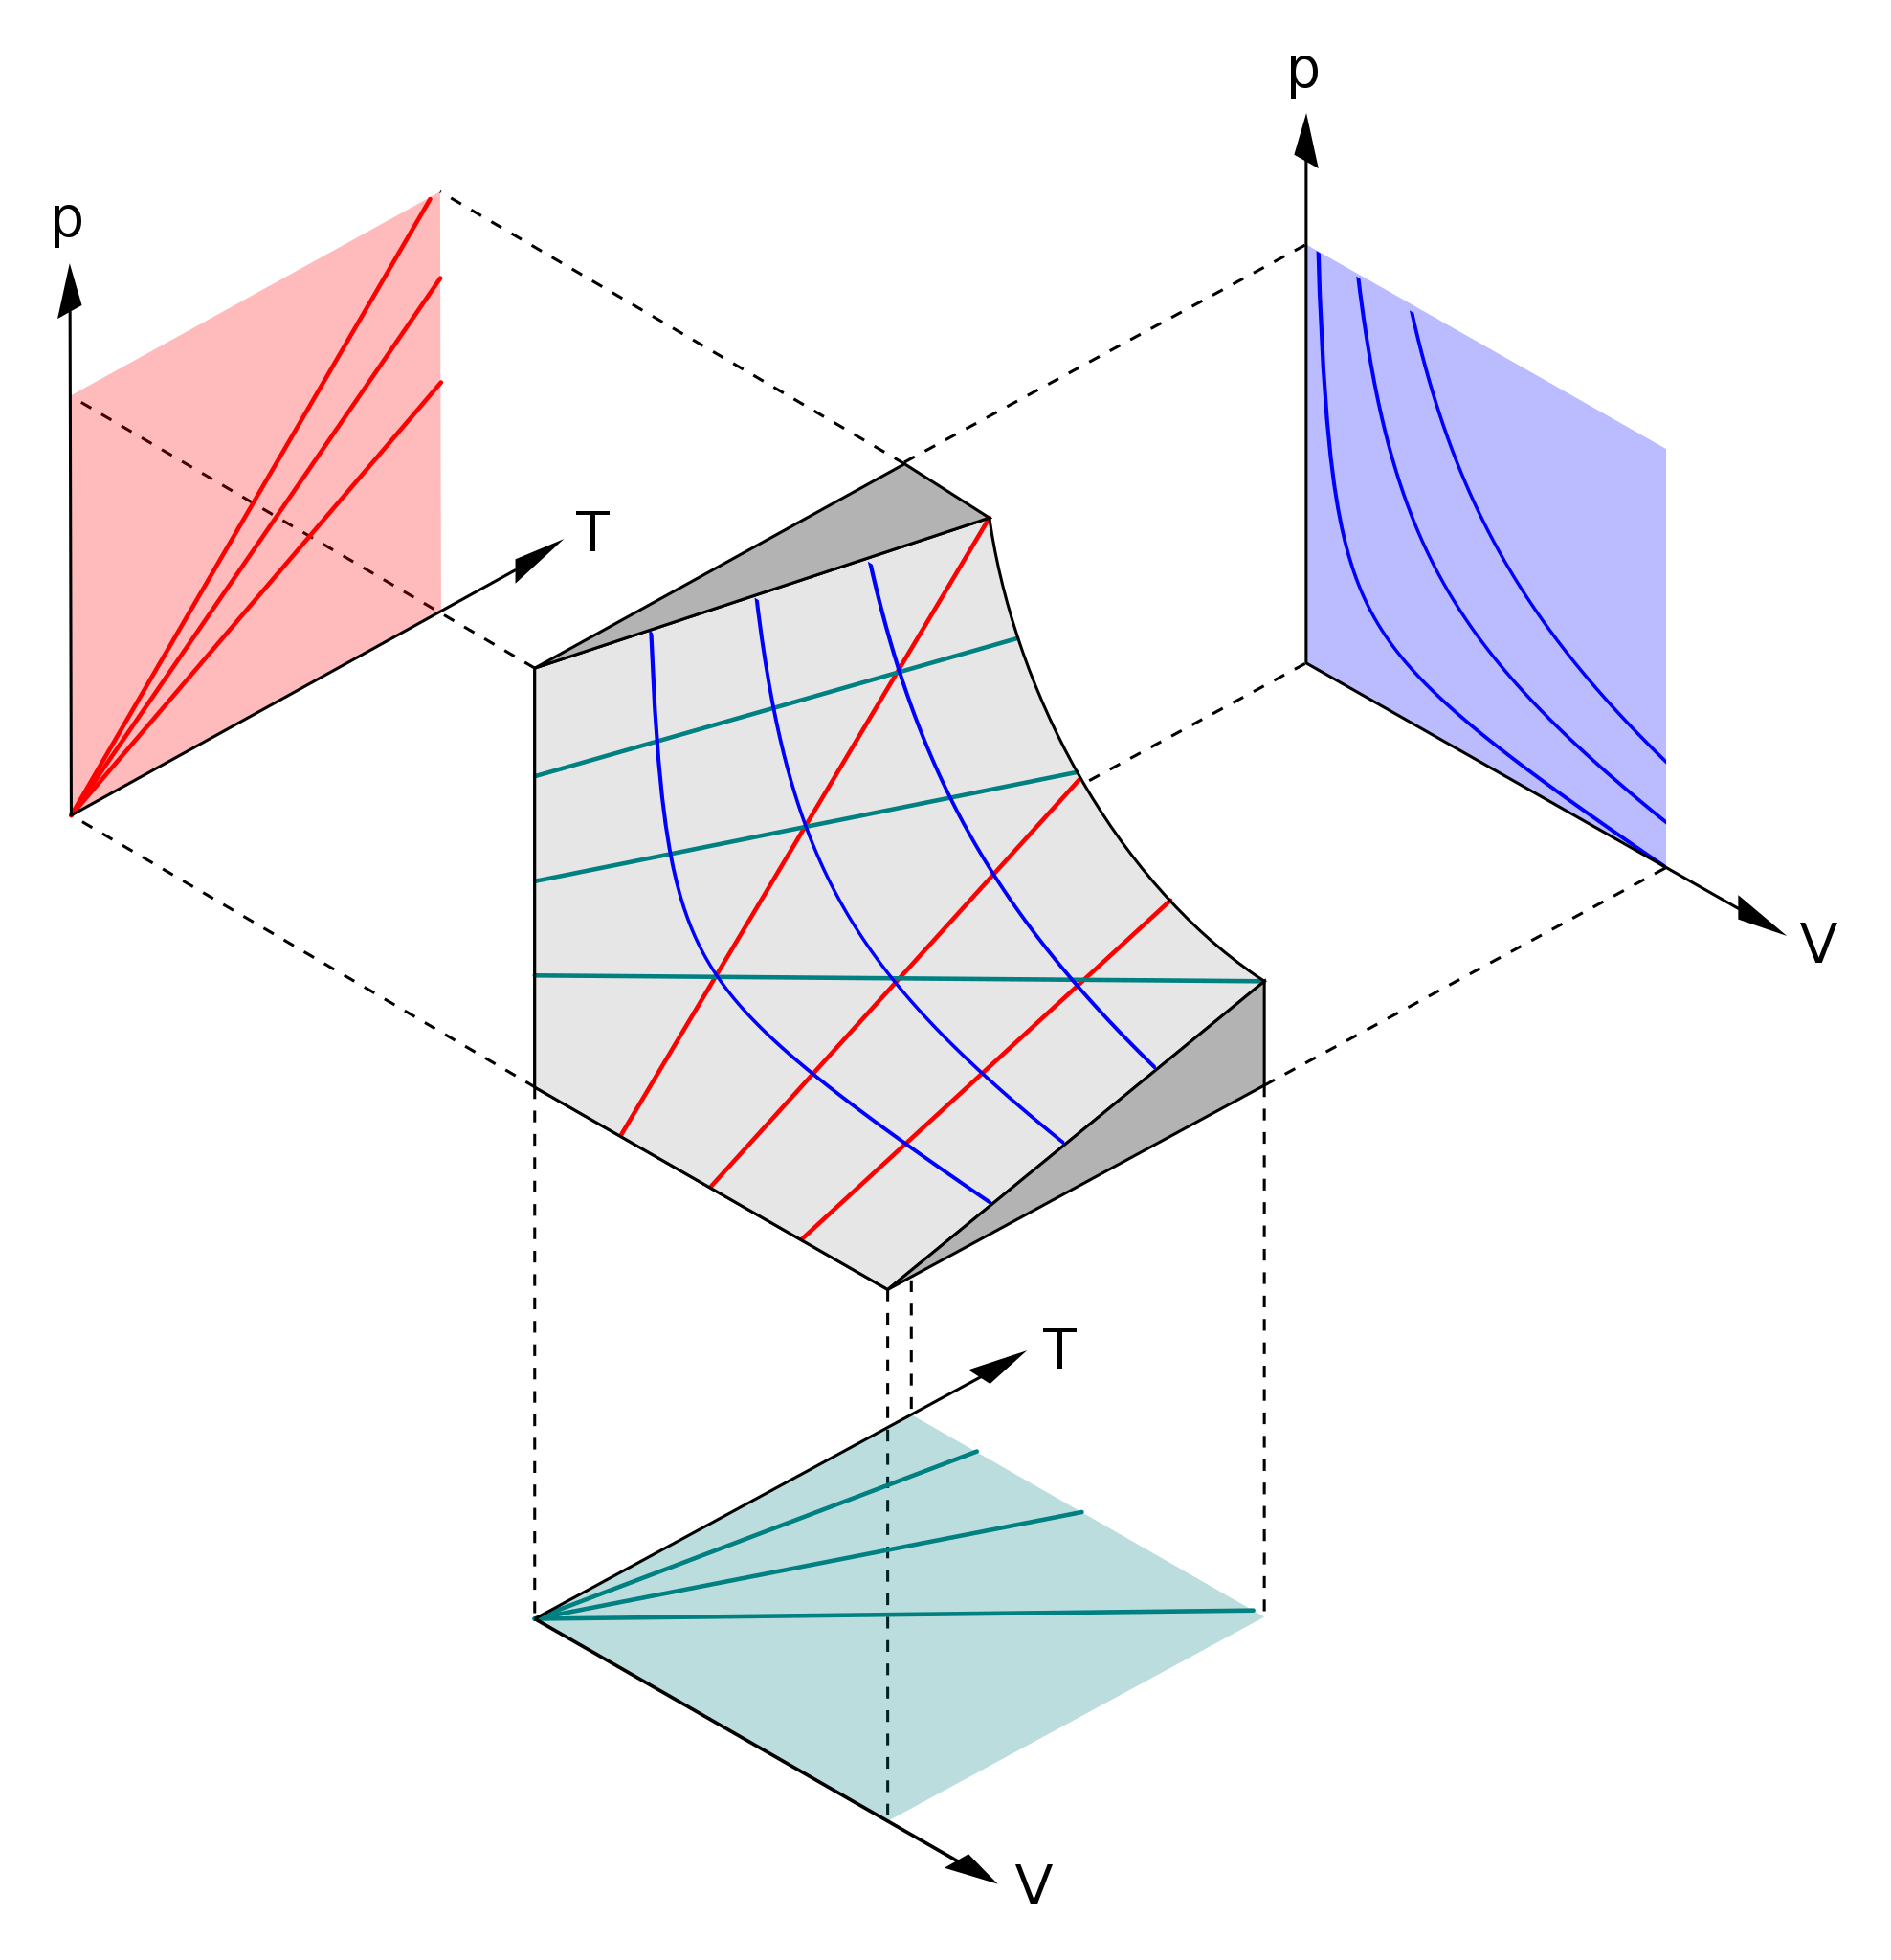
\includegraphics[width=14cm]{images/pVT-surface.png}
\end{figure}

\vocab{Mole} $n$: amount of substance that contains the same number of particles as the number of atoms in 0.012 kg (or 12 g) of carbon-12.

\vocab{Avogardo constant} $N_A$: number of particles in one mole of substance.
\[ N_A = \frac{N}{n} = 6.02 \times 10^{23} \: \unit{mol^{-1}} \]

\vocab{Boltzmann's constant}: gas constant per molecule.
\[ k_B = \frac{R}{N_A} = 1.38\times10^{-23} \: \unit{J.K^{-1}} \]

Rewriting the equation of state in \emph{number of molecules} gives us
\begin{equation}
pV=Nk_BT
\end{equation}

\vocab{Molar mass} of a substance $Mr$: mass of one mole of substance.
\[ Mr = \frac{m}{n} \]

\vocab{Molar volume} of a gas $V_m$: volume of one mole of gas.
\[ V_m = \frac{V}{n} \]
\pagebreak

\subsection{Kinetic theory of gases}
\textbf{Assumptions} of the kinetic theory of gases:
\begin{enumerate}
\item Gas consists of a very large number of particles.
\item Gas particles are in constant random motion and obey Newton's laws of motion.
\item No forces of attraction or repulsion between gas particles except during collision.
\item Gas particles behave as perfectly elastic, identical, hard spheres,
\item Total volume of the gas particles is negligible compared to volume of container.
\item Time duration of collision is negligible compared to time interval between collisions.
\end{enumerate}

Explain how molecular movement causes the pressure exerted by a gas.
\begin{itemize}
\item Gas molecules have rapid and random motion.
\item When they hit the walls of the container, they exert a force.
\item Pressure = Force/Area
\end{itemize}

We have the following relationship.
\begin{equation}
pV = \frac{1}{3}Nm\langle c^2 \rangle
\end{equation}

\deriv{See Appendix for the derivation.}

Related equations include
\[ pV=\frac{1}{3}Nm\langle c^2\rangle \iff \frac{1}{3}M\langle c^2\rangle \iff \frac{1}{3}nM_r\langle c^2\rangle \]

Using this, we can deduce the mean translational kinetic energy of one molecule.
\begin{equation}
\langle\text{KE}\rangle=\frac{1}{2}m\langle c^2\rangle = \frac{3}{2}k_BT
\end{equation}
This means that mean KE of a molecule of an ideal gas is \emph{proportional} to the thermodynamic temperature.

Thus total translational kinetic energy of $N$ molecules is given by
\begin{equation}
N\langle\text{KE}\rangle=\frac{3}{2}Nk_BT=\frac{3}{2}nRT
\end{equation}
\pagebreak

\subsection*{Problems}
\begin{prbm}
A resistance thermometer gives a resistance of 20 $\Omega$ when the temperature is known to be $-10$ \degree C. When the temperature is 110\degree C, the resistance thermometer has a resistance of 500 $\Omega$. What is the temperature when the resistance is 360 $\Omega$?
\end{prbm}
\begin{solution}
\[ \frac{\theta-(-10)}{110-(-10)}=\frac{360-20}{500-20} \implies \boxed{\theta=75\degree} \]
\end{solution}

\begin{prbm}
Two bulbs, $X$ of volume 100 \unit{cm^3} and $Y$ of volume 50 \unit{cm^3}, are connected with a tube of negligible volume. A valve prevents gas to flow between the two bulbs. Initially bulb $X$ is filled with an ideal gas at 10\degree C to a pressure of $3\times10^5$ Pa. Bulb $Y$ is filled with the same ideal gas at 100\degree C to a pressure of $1\times10^5$ Pa. The valve is opened and the temperature of $X$ and $Y$ are maintained at their initial temperatures. Determine the new equilibrium pressure of the system.
\end{prbm}
\begin{solution}
Both bulbs exchange molecules until pressure is equal.

Total number of particles is conserved.
\begin{align*}
n_{X,i}+n_{Y,i} &= n_{X,f}+n_{Y,f} \\
\frac{P_{X,i}V_x}{T_X}+\frac{P_{Y,i}V_Y}{T_Y} &= \frac{P_fV_X}{T_X}+\frac{P_fV_Y}{T_Y}
\end{align*}
$\therefore\quad \boxed{P_f=2.45 \times 10^5\:\unit{Pa}}$
\end{solution}
\pagebreak
\section{First Law of Thermodynamics}
\subsection{Specific Heat Capacity, Latent Heat}
\begin{defn}{Specific heat capacity $c$}{}
Quantity of heat required to raise the temperature of a unit mass of a substance by 1 \unit{K}.\todo{wait for lecture}
\begin{equation}
Q = mc\Delta T
\end{equation}
\end{defn}

\begin{defn}{Specific latent heat $L$}{}
\begin{equation}
Q = mL
\end{equation}
\end{defn}

\textbf{Phase change}: transition from one state of matter to another. During a phase change, latent heat is given off or absorbed, temperature of the object does not change.

\subsection{Internal Energy}
The \vocab{state} of a system is defined by its pressure $p$, volume $V$, and thermodynamic temperature $T$.\footnote{not solid, liquid or gas (there are \emph{phases}). The concept of state must be clear!}

\begin{defn}{Internal energy $U$}{}
Sum of \emph{kinetic energy} due to random motion of molecules, and \emph{potential energy} due to intermolecular forces of attraction.
\begin{equation}
U = \text{KE}_\text{random} + \text{PE}_\text{random}
\end{equation}
\end{defn}

For an ideal gas, no intermolecular attraction hence no random PE. Internal energy is only the sum of random distribution of KE of molecules.
\[ U = \text{KE}_\text{random} = N\langle\text{KE}\rangle = \frac{3}{2}Nk_BT \]
This means increase in temperature of an ideal gas indicates increase in mean random KE of molecules. This means an increase in sum of random KE, and thus increase in internal energy.

\subsection{First Law of Thermodynamics}
Work done $W$ is area under pressure-volume graph
\[ W=\int p \dd{V} \]

\begin{defn}{First Law of Thermodynamics}{}
Internal energy of a system depends only on its state. Internal energy of system is the sum of the heat supplied to system and work done on system.

\begin{equation}
\Delta U = Q_\text{to} + W_\text{on}
\end{equation}

where $\Delta U$ is the change in internal energy, $Q_\text{to}$ is heat supplied to system, $W$ is work done on the system.
\end{defn}

\subsubsection{Thermodynamic processes}
\textbf{Quasi-static process}: idealised process where the change in state is made infinitesimally slowly so that at each instant, the system can be assumed to be at a thermodynamic equilibrium with itself and with the environment.

The \textbf{state} of a system can be represented by a point on $p-V$ graph.

\textbf{Isotherm}: hyperbolic $p-V$ graph (since $pV$ is constant at constant temperature)

\begin{figure}[H]
    \centering
    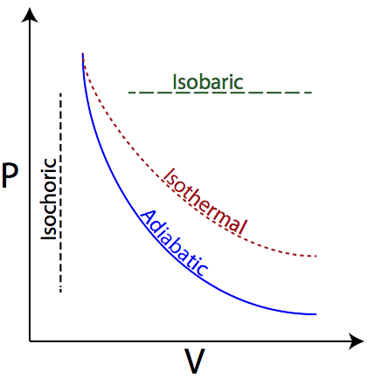
\includegraphics[width=0.5\textwidth]{images/thermodynamic_processes.png}
\end{figure}

\begin{itemize}
\item \vocab{Isothermal} expansion/contraction: \textbf{constant temperature}

Change in state occurs along an isotherm. Constant temperature implies constant mean random KE and hence constant total random KE of molecules. For an ideal gas, it means constant internal energy.

Both $p$ and $V$ change, but $pV$ is constant.

$\Delta U=0$

\item \vocab{Isobaric} expansion/contraction: \textbf{constant pressure}

Constant pressure means system's environment is not changing e.g. system experiences atmospheric pressure.

Final state is on a different isotherm, meaning temperature changes. Volume of changes.

Work done by system $=-W=p\Delta V$

\item \vocab{Isochoric} heating/cooling: \textbf{constant volume}

Constant volume means system is confined in a rigid container, implying zero work done by and on the system. 

Final state is on a different isotherm, meaning the temperature changes. Pressure also changes.

$W=0$

\item \vocab{Adiabatic} expansion/contraction: \textbf{no heat exchange between system and environment}

During adiabatic expansion, system does work by pushing back its environment. Since no heat is supplied to system for it to do the work, it uses its thermal energy, thus temperature decreases.

Final state is at lower isotherm than initial state. Pressure also decreases.

Paths for adiabatic changes are steeper than isotherms.

$Q=0$
\end{itemize}

Temperature change - $\Delta U$ change

Volume change - $W$ done


\textbf{Cyclic process}: system starts and ends with same state, no change in internal energy

% https://superphysics.sg/wp-content/uploads/2019/09/H2-Chapter-11-Thermal-Physics-Summary.pdf
\pagebreak

\part{Oscillation and Waves}
\section{Oscillations}
\vocab{Free oscillation}: object oscillates with constant amplitude, with no external force acting on it

\begin{defn}{Amplitude $x_0$}{}
Magnitude of \underline{maximum displacement} from equilibrium position. 
\end{defn}

\begin{defn}{Period $T$}{}
Time taken for one complete oscillation. 
\end{defn}

\begin{defn}{Frequency $f$}{}
Number of complete cycles per unit time.
\end{defn}

\begin{defn}{Angular frequency $\omega$}{}
Measure of the rate of change of phase angle of the body's motion with time with respect to the centre of its oscillation.
\begin{equation} \omega = 2 \pi f = \frac{2\pi}{T}\end{equation}
\end{defn}
\pagebreak

\subsection{Kinematics}
\textbf{Displacement-time}:

When the body is at equilibrium position at $t=0$,
\begin{equation} x = x_0 \sin \omega t \end{equation}

\begin{figure}[H]
\centering
\begin{tikzpicture}
  \begin{axis}%
    [axis lines=middle,
     enlargelimits={abs=0.2},
     xlabel = $t$,
     ylabel = $x$,
     ticks=none
    ]
    \addplot[domain=0:12.57,samples=50,smooth,red] {sin(deg(x))};
  \end{axis}
\end{tikzpicture}
\end{figure}

When the body is at extreme position at $t=0$,
\[ x = x_0 \cos \omega t \]

\textbf{Velocity-time}:
\begin{equation} v = v_0 \cos \omega t \end{equation}

\begin{figure}[H]
\centering
\begin{tikzpicture}
  \begin{axis}%
    [axis lines=middle,
    enlargelimits={abs=0.2},
     xlabel = $t$,
     ylabel = $v$,
     ticks=none
    ]
    \addplot[domain=0:12.57,samples=50,smooth,red] {cos(deg(x))};
  \end{axis}
\end{tikzpicture}
\end{figure}
\pagebreak
\textbf{Acceleration-time}:
\begin{equation} a=-a_0\sin\omega t \end{equation}

\begin{figure}[H]
\centering
\begin{tikzpicture}
  \begin{axis}%
    [axis lines=middle,
    enlargelimits={abs=0.2},
     xlabel = $t$,
     ylabel = $a$,
     ticks=none
    ]
    \addplot[domain=0:12.57,samples=50,smooth,red] {-sin(deg(x))};
  \end{axis}
\end{tikzpicture}
\end{figure}

\textbf{Velocity-displacement}:
\begin{equation} v = \pm \omega \sqrt{{x_0}^2 - x^2} \end{equation}

\begin{figure}[H]
\centering
\begin{tikzpicture}
  \begin{axis}%
    [axis lines=middle,
    enlargelimits={abs=0.2},
     xlabel = $x$,
     ylabel = $v$,
     ticks=none,
     trig format plots=rad,variable=t
    ]    
    \addplot[domain=-2*pi:2*pi,samples=50,smooth,red]({10*cos(t)},{sin(t)});
  \end{axis}
\end{tikzpicture}
\end{figure}

\textbf{Acceleration-displacement}:\footnote{This is known as the defining equation of simple harmonic motion.}
\begin{equation} a = -\omega^2 x \end{equation}

\begin{figure}[H]
\centering
\begin{tikzpicture}
  \begin{axis}%
    [axis lines=middle,
    enlargelimits={abs=0.2},
     xlabel = $x$,
     ylabel = $a$,
     ticks=none
    ]    
    \addplot[domain=-6:6,samples=50,smooth,red] {-x};
  \end{axis}
\end{tikzpicture}
\end{figure}
\pagebreak

\begin{defn}{Phase}{}
Angle which gives a measure of the fraction of a cycle that has been completed by the oscillating particle or wave. 
\end{defn}

\begin{defn}{Phase difference $\phi$}{}
Angle which gives a measure of how much one oscillation is \underline{out of step} with another.
\end{defn}

\begin{itemize}
\item Graph of $x=x_0\cos(\omega t+\phi)$ is displaced to the left. Motion \textbf{leads} by time $\dfrac{\phi}{\omega}$.
\item Graph of $x=x_0\cos(\omega t-\phi)$ is displaced to the right. Motion \textbf{lags} by time $\dfrac{\phi}{\omega}$.
\end{itemize}

\begin{figure}[H]
\centering
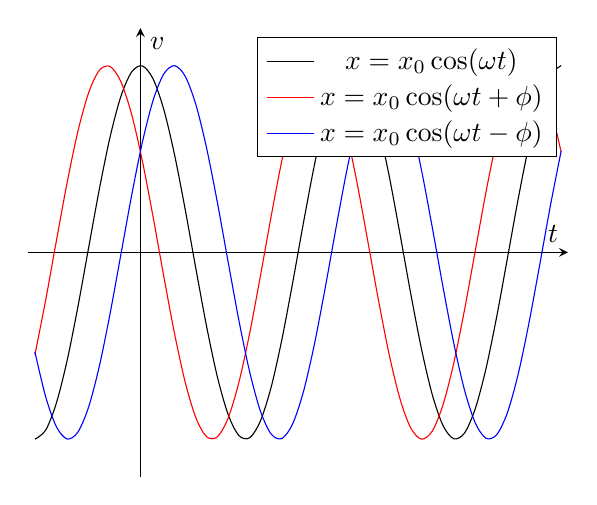
\begin{tikzpicture}
  \begin{axis}%
    [axis lines=middle,
    enlargelimits={abs=0.2},
     xlabel = $t$,
     ylabel = $v$,
     ticks=none
    ]
    \addplot[domain=-3.15:12.57,samples=50,smooth,black] {cos(deg(x))};
    \addlegendentry{$x=x_0\cos(\omega t)$}
    \addplot[domain=-3.15:12.57,samples=50,smooth,red] {cos(deg(x+1))};
    \addlegendentry{$x=x_0\cos(\omega t+\phi)$}
    \addplot[domain=-3.15:12.57,samples=50,smooth,blue] {cos(deg(x-1))};
    \addlegendentry{$x=x_0\cos(\omega t-\phi)$}
  \end{axis}
\end{tikzpicture}
\end{figure}
\pagebreak

\subsection{Energy}
For an oscillator in simple harmonic motion, total energy is sum of \textbf{kinetic energy} and \textbf{potential energy}.
\[ E=E_k+E_p \]
\begin{equation}
E_k = \frac{1}{2}m\omega^2{x_0}^2\cos^2 \omega t = \frac{1}{2}m\omega^2\brac{{x_0}^2-x^2}
\end{equation}
\begin{equation}
E_p = \frac{1}{2}m\omega^2{x_0}^2\sin^2 \omega t = \frac{1}{2}m\omega^2 x^2
\end{equation}
\[ E=E_{k,max}=E_{p,max}=\frac{1}{2}m\omega^2{x_0}^2 \]

Energy-time graph (for one period):
\begin{figure}[H]
\centering
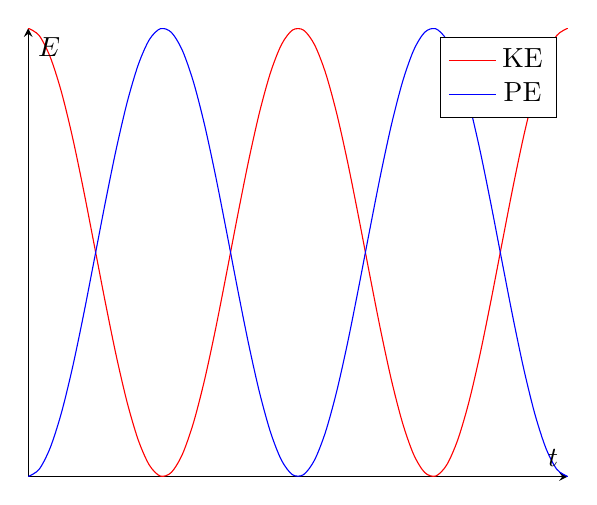
\begin{tikzpicture}
  \begin{axis}%
    [axis lines=middle,
     xlabel = \(t\),
     ylabel = {\(E\)},
     ticks=none
    ]
    \addplot[domain=0:12.57,samples=50,smooth,red] {cos(deg(x))+1};
    \addlegendentry{KE}
    \addplot[domain=0:12.57,samples=50,smooth,blue] {-cos(deg(x))+1};
    \addlegendentry{PE}
  \end{axis}
\end{tikzpicture}
\end{figure}

Energy-displacement graph (for one period):
\begin{figure}[H]
\centering
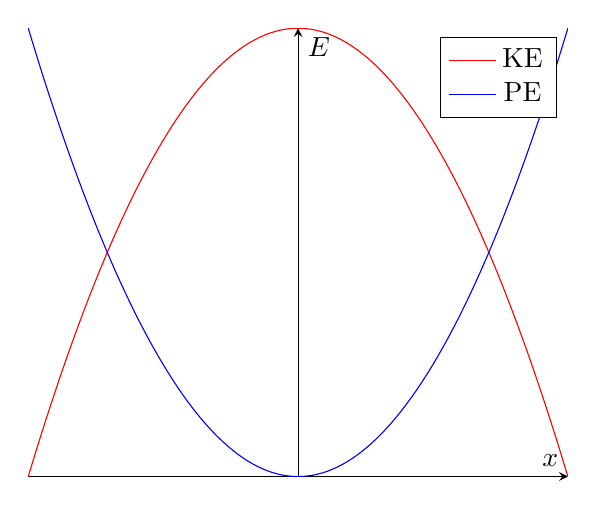
\begin{tikzpicture}
  \begin{axis}%
    [axis lines=middle,
     xlabel = \(x\),
     ylabel = {\(E\)},
     ticks=none
    ]
    \addplot[domain=-1:1,samples=50,smooth,red] {-x^2+1};
    \addlegendentry{KE}
    \addplot[domain=-1:1,samples=50,smooth,blue] {x^2};
    \addlegendentry{PE}
  \end{axis}
\end{tikzpicture}
\end{figure}
\pagebreak

\subsection{Simple harmonic motion}
\begin{defn}{Simple harmonic motion}{}
Oscillatory motion where acceleration is \underline{directly proportional} to displacement from a \underline{fixed point}, and this acceleration is always in the \underline{opposite direction} to its displacement.
\[ a \propto -x \]
\end{defn}

\subsubsection{Examples}
\textbf{Spring-mass system}

\begin{figure}[H]
    \centering
    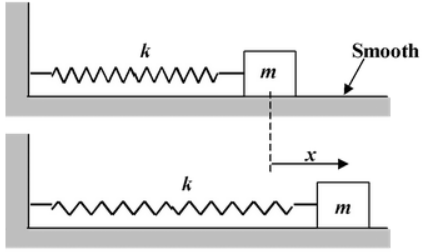
\includegraphics[width=8cm]{images/spring_mass_shm.png}
    \caption{Spring-mass system}
\end{figure}

Restoring force is $F=-kx$. By Newton's 2nd law, 
\[ \sum F=ma=-kx \implies a=-\frac{k}{m}x \]
Comparing with $a=-\omega^2x$,
\[ \omega = \sqrt{\frac{k}{m}} \]
Hence frequency is
\[ f=\frac{1}{2\pi}\sqrt{\frac{k}{m}} \]
\pagebreak

\textbf{Simple pendulum}

\begin{figure}[H]
    \centering
    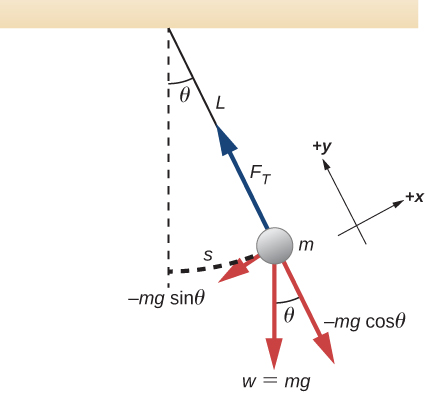
\includegraphics[width=8cm]{images/simple_pendulum_shm.jpg}
    \caption{Simple pendulum}
\end{figure}

Restoring force is the component of the bob's weight, $mg\sin\theta$, that is tangential to the circumference of its swing. 

For small $\theta$, by small angle approximation, $mg\sin\theta \approx mg\theta$, where $\theta\approx\frac{x}{l}$.

By Newton's 2nd Law, 
\[ \sum F=ma=-mg\theta=-\frac{mgx}{l} \implies a=-\frac{g}{l}x \]

Comparing with $a=-\omega^2x$,
\[ \omega=\sqrt{\frac{g}{l}} \]

Hence frequency is
\[ f=\frac{1}{2\pi}\sqrt{\frac{g}{l}} \]
This indicates that the angular velocity or the period of a simple pendulum is independent of the mass of the weight and the amplitude of oscillation. This is called Galileo's \textbf{isochronism of pendulum}.
\pagebreak

\textbf{Vertical spring-mass system}

\begin{figure}[H]
    \centering
    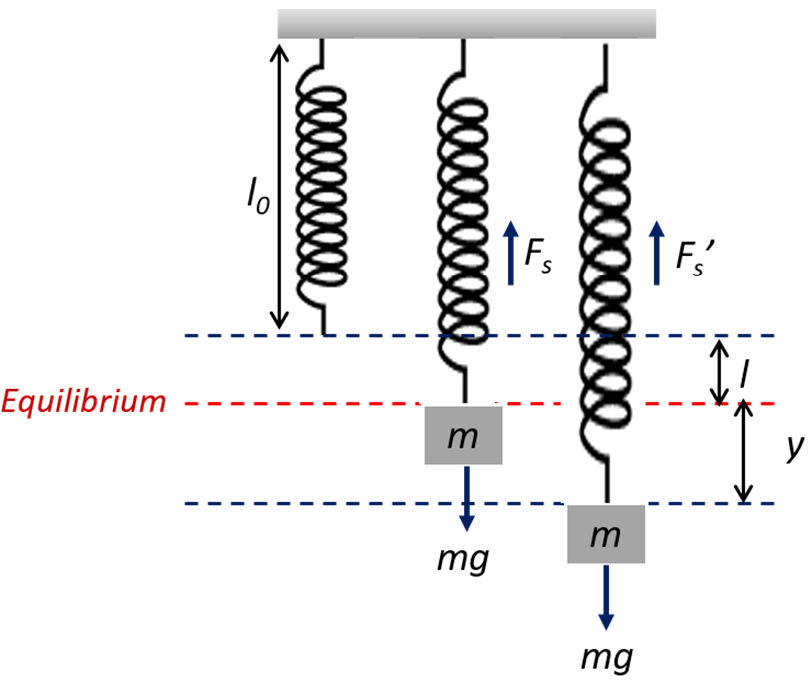
\includegraphics[width=8cm]{images/vertical_spring_mass_shm.png}
    \caption{Vertical spring-mass system}
\end{figure}

At equilibrium, spring force balances weight: $ke=mg$.

At lowest point, by Newton's 2nd law,
\[ \sum F=mg-k(e+x)=ma \implies a=-\frac{k}{m}x \]

Comparing with $a=-\omega^2x$,
\[ \omega^2=\frac{k}{m} \implies f=\frac{1}{2\pi}\sqrt{\frac{k}{m}} \]
\pagebreak

\textbf{Floating block}

\begin{figure}[H]
    \centering
    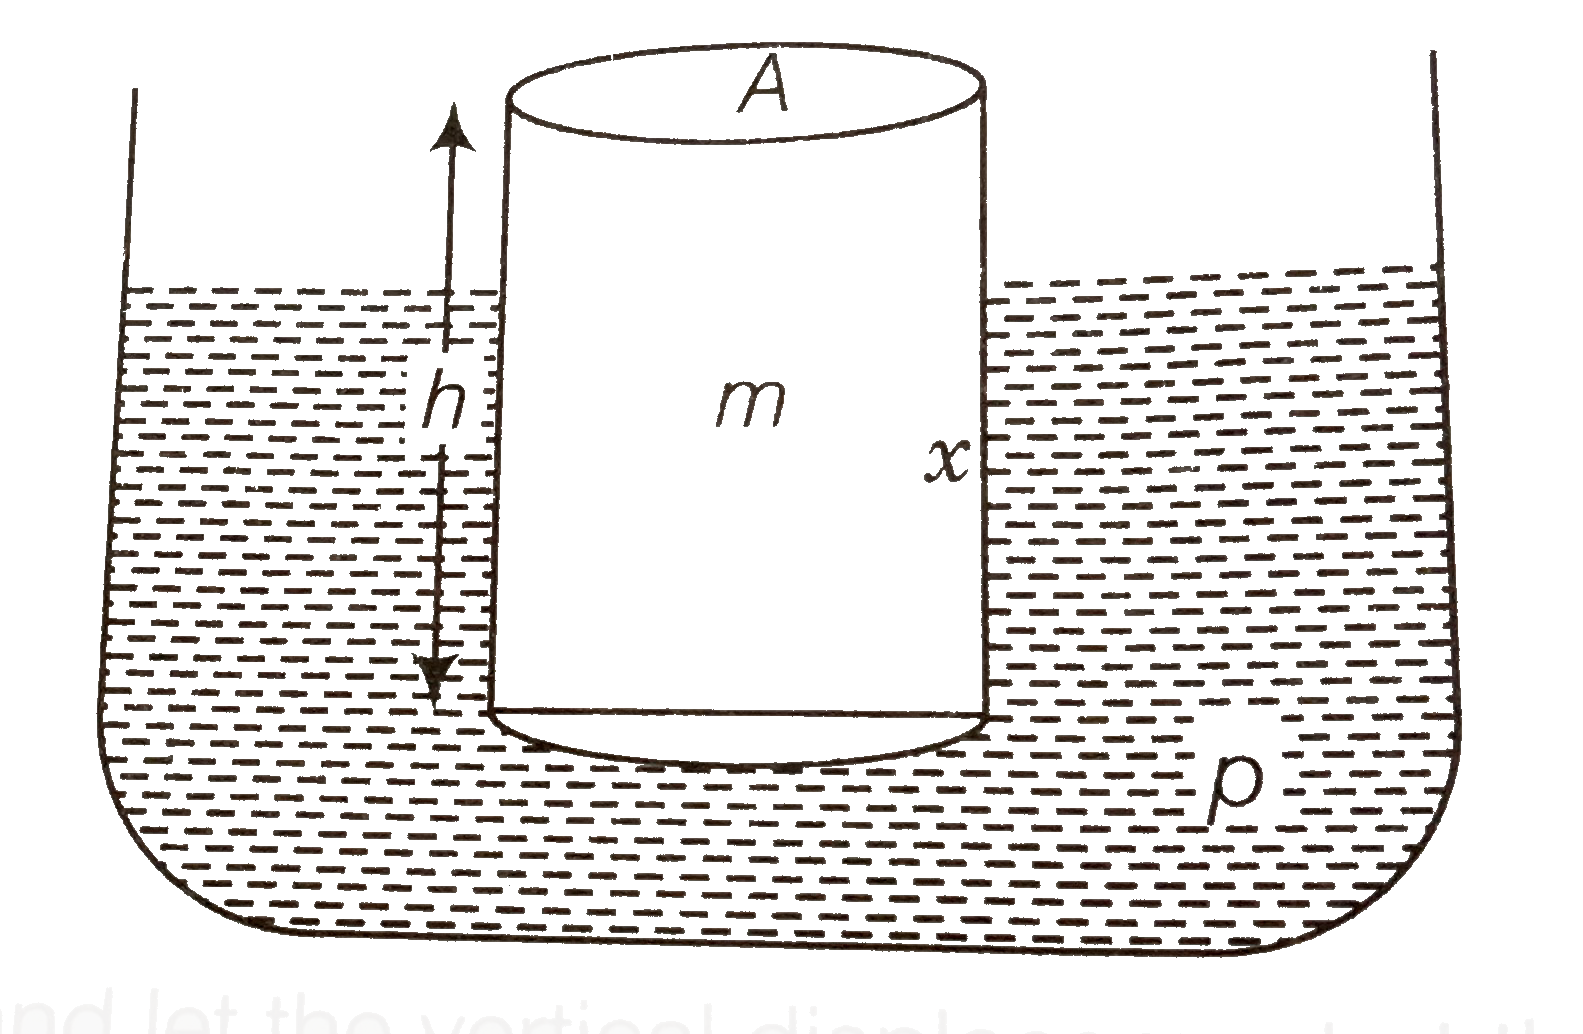
\includegraphics[width=8cm]{images/floating_block_shm.png}
    \caption{Floating block}
\end{figure}

Restoring force is the difference between upthrust exerted by water on block and the block's weight. By Newton's 2nd law,
\[ \sum F=mg-\rho(A(h+x))g = -\rho(Ax)g = ma \implies a=-\frac{\rho Ag}{m}x \]

Comparing with $a=-\omega^2x$,
\[ \omega=\sqrt{\frac{\rho Ag}{m}} \]
Hence frequency is 
\[ f=\frac{1}{2\pi}\sqrt{\frac{\rho Ag}{m}} \]
\pagebreak


\subsection{Damped oscillation}
\begin{defn}{Damping}{}
\underline{Energy is lost} from system as a result of \underline{dissipative forces.}
\end{defn}

\begin{defn}{Damped oscillation}{}
\underline{Amplitude decreases with time} due to loss of energy to surroundings as a result of resistive forces acting on system.
\end{defn}

Degrees of damping:
\begin{enumerate}
\item \textbf{Light damping}: continues to oscillate, amplitude decreases gradually with time but period remains almost the same
\item \textbf{Heavy damping}: does not oscillate, takes a long time to return to equilibrium\\ e.g. door damper
\item \textbf{Critical damping}: does not oscillate, returns to equilibrium in the shortest possible time\\ e.g. damping system of car
\end{enumerate}

\begin{figure}[H]
    \centering
    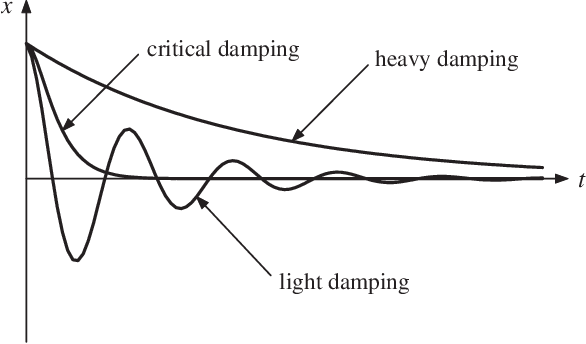
\includegraphics[width=11cm]{images/Damping.png}
\end{figure}

The equation for undamped free oscillation is 
\[ x=x_0\cos\omega t \]
The equation for damped oscillation is 
\[ x=x_0e^{-\frac{b}{2m}t}\cos\omega t \]
where $b$ is the damping constant.
\pagebreak

\subsection{Forced oscillation}
\begin{defn}{Forced oscillation}{}
Continual \underline{input of energy} by an external applied force, to compensate the energy loss due to damping, in order to maintain amplitude of oscillation.

The system oscillates at the frequency of the external periodic force.
\end{defn}

\subsection{Resonance}
\begin{defn}{Natural frequency $f_0$}{}
Frequency at which a body oscillates after an initial disturbance. 
\end{defn}

\begin{defn}{Resonance}{}
Amplitude of the oscillator reaches a maximum when driving frequency equals natural frequency of the oscillator, resulting in maximum transference of energy to the oscillator.
\[ f=f_0 \]
\end{defn}

Amplitude of forced oscillation changes with driving frequency. When $f=f_0$, \underline{resonance} occurs, amplitude is maximum.

\begin{figure}[H]
    \centering
    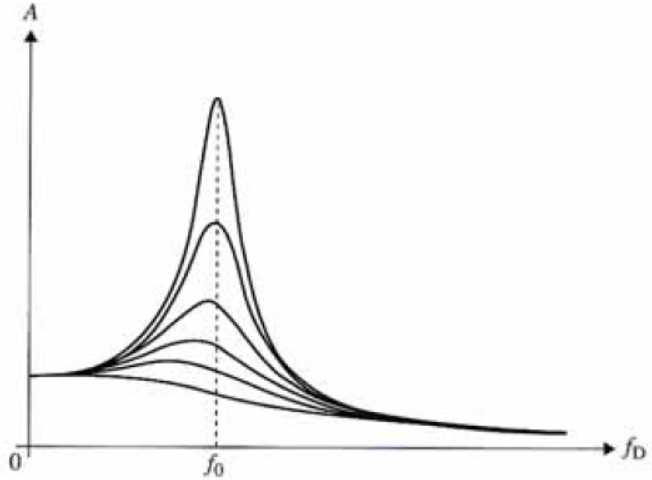
\includegraphics[width=10cm]{images/Amptlitude_forced_oscillation.png}
\end{figure}

Effect of increased damping on resonance curve:
\begin{itemize}
\item Lower at all frequencies
\item Flatter peak
\item Peak shifts to left slightly
\end{itemize}

\textbf{Applications of resonance:} magnetic resonance imaging (MRI)

\textbf{Drawbacks of resonance:} bridge design to prevent collapse due to resonant oscillations
\pagebreak

\subsection*{Problems}
\begin{prbm}
A cylinder of radius $R$, length $h$, density $\rho_0$ floats upright in a fluid of density $\rho_1$. It is given a small vertical displacement, and undergoes undamped harmonic motion with angular frequency $\omega$. 

Calculate $\omega^2$.
\end{prbm}

\begin{proof}[Solution]
Using Archimedes’ principle: the force on the cylinder is equal to the weight of the water displaced, which is
\[ F = mg = -\rho_1 (\pi R^2 d)g \]
where $d$ is the vertical displacement. 

This acts as a spring force $F=-kd$. The spring constant $k$ of a harmonic oscillator of mass $m$ is related to the angular frequency $\omega$ by $k=m\omega^2$; in this case, mass $m=\rho_0 \cdot \pi R^2h$.

Putting everything together, 
\[ k=\rho_1\pi R^2 g = \rho_0\pi R^2 h\omega^2 \]
\[ \boxed{\omega^2=\frac{\rho_1g}{\rho_0h}} \]
\end{proof}
\pagebreak

\begin{prbm}
The figure below shows a simple pendulum consisting of a small mass at the end of a light, inextensible string. It swings from an initial position of $\theta=10\degree$, for which it would have a period $T_0$. It hits a slanted wall elastically, which is at angle $\phi=5\degree$ to the vertical.

\begin{figure}[H]
    \centering
    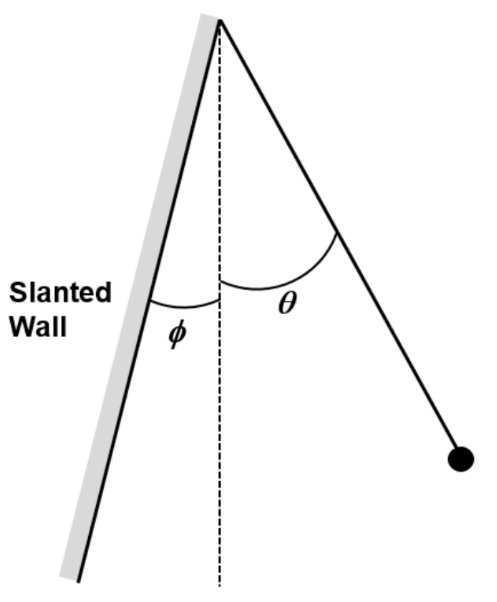
\includegraphics[width=6cm]{images/pendulum_wall.png}
\end{figure}

When the pendulum hits the wall, what is the new period of oscillation, in terms of $T_0$?
\end{prbm}

\begin{proof}[Solution]
Simple harmonic motion implies $\theta = \theta_0 \cos \omega t$, where $\theta_0 = 10\degree$ before the collision, and given the period we know $\omega = \dfrac{2\pi}{T_0}$.

Let $T$ be time taken to swing from initial position to $-5\degree$.
\[ -5\degree = 10\degree \cos \frac{2\pi T}{T_0} \implies \frac{2\pi T}{T_0} = \frac{2\pi}{3} \implies T=\frac{T_0}{3} \]

Hence new period is $\boxed{\dfrac{2T_0}{3}}$.
\end{proof}

\pagebreak
\section{Wave Motion}
\subsection{Progressive Waves}
\begin{defn}{Progressive wave}{}
Wave in which energy is carried from one point to another \emph{by means of vibrations or oscillations} within the waves, without transporting matter.
\end{defn}

\subsubsection{Key Terms}
\begin{defn}{Displacement $y$}{}
Distance in a specific direction of a point on the wave from its equilibrium position.
\end{defn}

\begin{defn}{Amplitude $A$}{}
Maximum displacement of any point on the wave from its equilibrium position. 
\end{defn}

\begin{defn}{Period $T$}{}
Time taken for one complete oscillation of a point in the wave.

(Time taken for wave to travel a distance of one wavelength)
\end{defn}

\begin{defn}{Frequency $f$}{}
Number of oscillations per unit time of a point on the wave.
\end{defn}

\begin{defn}{Wavelength $\lambda$}{}
Minimum distance between any two points of the wave with the \emph{same phase} at the \emph{same instant}.
\end{defn}

\begin{defn}{Wave speed $v$}{}
Speed with which energy is transmitted by wave.
\begin{equation}
v=f\lambda
\end{equation}
\end{defn}

\begin{remark}
For EM waves, $v=3\times10^8$ \unit{m.s^{-1}} in vacuum; for sound waves, $v=330$ \unit{m.s^{-1}} in air.
\end{remark}

\begin{defn}{Wavefront}{}
An imaginary line or surface joining points that are in phase.
\end{defn}

\subsubsection{Transverse and Longitudinal Waves}
\begin{defn}{Transverse wave}{}
Direction of vibration of the wave particles is \underline{perpendicular} to \emph{direction of transfer of energy} of the wave.
\end{defn}

\begin{defn}{Longitudinal wave}{}
Direction of vibration of the wave particles is \underline{parallel} to the \emph{direction of transfer of energy} of the wave.
\end{defn}

\textbf{Mechanical wave}: wave that requires a medium for propagation.
E.g.: sound waves, Water waves

\textbf{Electromagnetic wave}: wave consisting of oscillating electric and magnetic fields that are perpendicular to each other and to the direction of transfer of energy of wave. It does not require medium for transmission. It can travel through a vacuum at spedd of light.

\subsubsection{Graphical Representations}
\begin{itemize}
\item \textbf{Displacement-distance graph}

Displacement of particles at a particular instant in time.

Determine wavelength, amplitude

\item \textbf{Displacement-time graph}

Displacement of a single particle varies with time.

Determine period, amplitude

\item \textbf{Pressure-distance graph} (longitudinal waves)
\end{itemize}

\subsubsection{Phase and Phase Difference}
\textbf{Phase}: angle which indicates fraction of a cycle completed by particle / wave.

\textbf{Phase difference} $\Delta\phi$: angle which indicates how much one wave / particle is \emph{out of step} with another.
\begin{itemize}
\item \textbf{In phase}: in step with one another ($\Delta\phi=0$)
\item \textbf{Out of phase}: not in step with one another ($\Delta\phi\neq0$)
\item \textbf{Anti-phase}: out of phase by half cycle ($\Delta\phi=\pi$)
\end{itemize}

For displacement-distance graph,
\begin{equation}
\Delta\phi = \frac{\Delta x}{\lambda} \times 2\pi
\end{equation}

For displacement-time graph,
\begin{equation}
\Delta\phi = \frac{\Delta t}{T} \times 2\pi
\end{equation}

\subsubsection{Energy, Intensity}
From SHM, energy associated with oscillation is proportional to square of amplitude:
\[ E = \frac{1}{2}m\omega^2{x_0}^2 = \frac{1}{2}m(2\pi f)^2{x_0}^2 \implies \boxed{E\propto f^2A^2} \]

\begin{defn}{Intensity $I$}{}
Rate of energy transmitted per unit area perpendicular to direction of wave velocity.
\begin{equation}
I = \frac{P}{\text{Area}}
\end{equation}
\end{defn}

As a wave spreads out, its amplitude decreases. This suggests that intensity $I$ of a wave is related to amplitude $A$. At constant $f$,
\[ I\propto E \text{ and } E\propto A^2 \implies \boxed{I\propto A^2} \]

Sources of transmission
\begin{itemize}
\item Three-dimensional transmission: point source emits energy radially outwards onto spherical surface (surface area of $4\pi r^2$)
\[ I\propto\frac{1}{r^2} \]
\item Two-dimensional transmission: point source emits energy radially outwards onto cylindrical surface (surface area of $2\pi rh$)
\[ I\propto\frac{1}{r} \]
\end{itemize}
\pagebreak

\subsection{Polarisation}
\begin{defn}{Polarisation}{}
Oscillations of wave are \emph{confined to only one direction}, in the plane normal to the direction of transfer of energy of wave.
\end{defn}

\begin{remark}
Polarisation is associated only with \emph{transverse waves}. Longitudinal waves (e.g. sound waves) cannot be polarised, as they do not have oscillations in the plane normal to direction of transfer of energy of wave.
\end{remark}

\textbf{Polariser}: optical filter that allows waves of specific polarisation pass through, while blocking waves of other polarisation.

\begin{figure}[H]
    \centering
    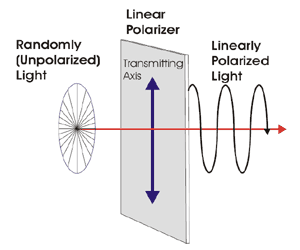
\includegraphics[width=8cm]{images/polarisation.png}
\end{figure}

\subsubsection{One Polariser}
When an unpolarised wave is incident on a polariser, its intensity is halved\footnote{because incident unpolarised wave is a random mixture of all states of polarisation, so vertical and horizontal components are, on average, equal.}, amplitude unchanged.
\begin{equation}
I=\frac{1}{2}I_0
\end{equation}

\subsubsection{Two Polarisers}
Analyser only allows \emph{component} of oscillation \emph{parallel} to transmission axis to pass through.

\begin{figure}[H]
    \centering
    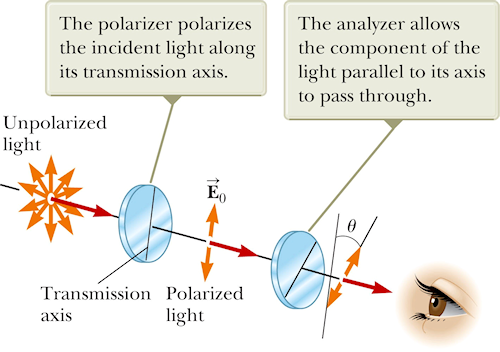
\includegraphics[width=10cm]{images/polariser_two.png}
\end{figure}

Let $I_0$ denote intensity of linearly polarised light, $I$ denote intensity after passing through analyser, $\theta$ denotes angle between direction of polarisation of incident wave and the polarising axis. Then
\begin{equation*}\tag{1}
I_0 \propto {A_0}^2
\end{equation*}
Component of $A_0$ parallel to transmission axis of analyser is $A=A_0\cos\theta$. Hence $I \propto (A_0\cos\theta)^2$, or
\begin{equation*}\tag{2}
I \propto {A_0}^2\cos^2\theta
\end{equation*}

Dividing (2) by (1) and rearranging gives \textbf{Malus' Law}:
\begin{equation}
I = I_0\cos^2\theta
\end{equation}

\begin{remark}
$I$ is maximum when transmission axes of polariser and analyser are aligned, i.e. $\theta=0\degree$; $I$ is minimum when transmission axes are perpendicular to each other, i.e. $\theta=90\degree$.
\end{remark}
\pagebreak

\subsection{Cathode Ray Oscilloscope (c.r.o.)}

\begin{figure}[H]
    \centering
    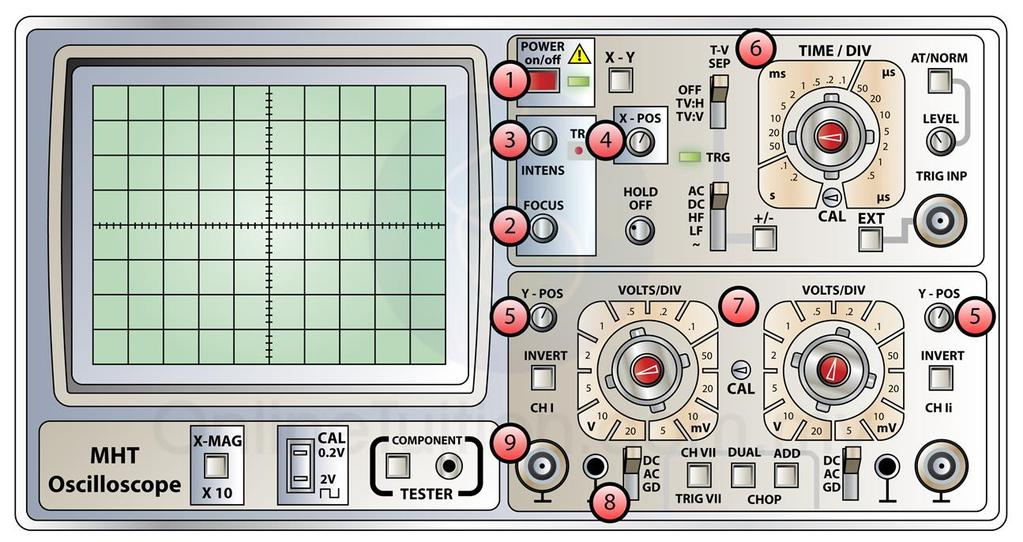
\includegraphics[width=10cm]{images/cro.jpg}
\end{figure}

Determine frequency of sound wave
\begin{enumerate}
\item Signal fed through microphone into c.r.o.
\item Turn on time-base of c.r.o., trace on screen displays displacement against time.
\item Adjust time-base until stationary trace obtained.
\item Find period $T$, calculate frequency $f$ using $f=\dfrac{1}{T}$.
\end{enumerate}

Determine wavelength of sound wave (using stationary waves)
\begin{enumerate}
\item Loudspeaker delivers sound via signal generator. Incident wave is directed towards and is reflected at reflecting board.
\item Superposition of incident wave and reflected wave produces stationary wave in the space between loudspeaker and reflecting board.
\item Connect microphone to c.r.o. (time-base switched off\footnote{so that the spot does not move across the screen. The spot moves up and down the screen, and the height of the vertical trace gives a measure of the amplitude of the sound}). Move it along the line between loudspeaker and reflecting board.
\item When microphone is at positions of minimum amplitude (nodes), signal displayed is minimum; at positions of maximum amplitude (antinodes), signal displayed is maximum.
\item Measure distance across several nodes / antinodes, calculate average distance $d$ between two adjacent nodes / antinodes.
\item Separation of two adjacent nodes is equal to half a wavelength: $d=\dfrac{1}{2}\lambda$.
\end{enumerate}

\begin{figure}[H]
    \centering
    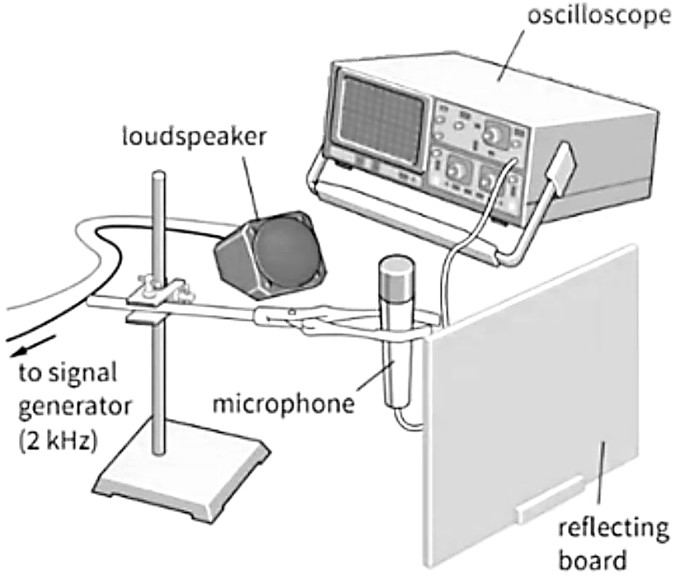
\includegraphics[width=10cm]{images/cro_wavelength.jpg}
\end{figure}

\begin{exercise}{}{}
Suggest why it is easier to determine accurately the position of a node rather than an antinode.
\end{exercise}
\begin{proof}[Answer]
The amplitude of oscillation at a node is zero. Hence it is easier to see the spot on the screen lie right on the horizontal line.
\end{proof}

\begin{exercise}{}{}
Explain why it is better to measure the distance across several nodes.
\end{exercise}
\begin{proof}[Answer]
Measuring a longer distance produces a smaller relative error of measurement.
\end{proof}

\pagebreak

\subsection*{Problems}
% https://www.topperlearning.com/answer/two-polarizers-are-placed-at-crossed-position-ie-having-an-angle-of-90-between-them-a-third-polarizer-making-an-angle-with-the-first-one-is-placed-bet/jbjws733
\pagebreak
\section{Superposition}
\subsection{Principle of Superposition}
\begin{defn}{Principle of superposition}{}
When two or more waves of the \emph{same type} meet at a point at the same time, the displacement of the resultant wave is the \underline{vector sum} of the displacements of the individual waves at that point at that time.
\end{defn}

\subsection{Stationary Waves}
\begin{defn}{Node}{}
Region of destructive superposition where the two waves meet antiphase.

Displacement is permanently zero (or minimum amplitude).
\end{defn}

\begin{defn}{Antinode}{}
Region of constructive superposition where the two waves meet in phase. 

Displacement is maximum amplitude.
\end{defn}

Distance between two adjacent nodes / antinodes:
\[ d=\frac{1}{2}\lambda \]

\begin{defn}{Stationary wave}{}
A stationary wave is formed when two progressive waves of the \emph{same type} of \emph{equal amplitude}, \emph{equal frequency}, \emph{equal speed} travelling in opposite directions meet and undergo superposition with each other.
\end{defn}

\begin{itemize}
\item Wave profile does not advance.
\item Positions of wave elements oscillating with maximum amplitudes (antinodes) and minimum amplitudes (nodes) are fixed with time. 
\item Vibrational energy of the wave is not transmitted from one point to another.
\end{itemize}

Progressive vs stationary waves
\begin{table}[H]
\centering
\begin{tabular}{|p{2cm}|p{6.5cm}|p{6.5cm}|}
\hline
& \textbf{Progressive wave} & \textbf{Stationary wave} \\
\hline
Amplitude & Same amplitude for all particles in wave motion & Amplitude of oscillating particles varies from zero (at node) to a maximum (at antinode) \\
\hline
Frequency & Particles vibrate in SHM with frequency of progressive wave & Particles vibrate in SHM with frequency of stationary wave \\
\hline
Wavelength & Shortest distance between two points in phase & Twice the distance between a pair of adjacent nodes / antinodes \\
\hline
Phase & All particles within one wavelength have different phases & All particles within a loop vibrate in phase, paricles in adjacent loops are antiphase \\
\hline
Wave profile & Wave profile advances with the speed of wave & Wave profile does not advance \\
\hline
Energy & Energy is transported in the direction of travel of wave & Energy is stored within vibratory motion of stationary wave \\
\hline
\end{tabular}
\end{table}

Drawing of stationary waves: (draw the two extremes)


\subsubsection{Transverse stationary waves}
\paragraph{Stretched string}

\textbf{Experiment set-up:} String of length $L$ is stretched tightly between fixed supports. When plucked, progressive wave produces, reflected at fixed ends, travel backwards. Incident and reflected waves superpose to form a stationary wave.

\textbf{Node}: fixed ends

\begin{table}[H]
  \centering
  \begin{tabular}{|c|c|c|c|c|}
    \hline
    \textbf{Mode of vibration} & \textbf{Wavelength} & \textbf{Frequency} & \textbf{Harmonic} & \textbf{Overtone}\\
    \hline
    \begin{minipage}{.3\textwidth}
      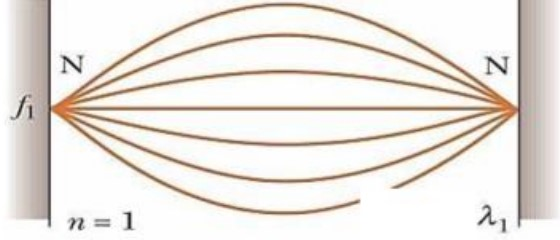
\includegraphics[width=\linewidth, height=30mm]{images/stretched_string_1.jpg}
    \end{minipage}
    & $\lambda_1=2L$ & $f_1=\dfrac{v}{\lambda_1}=\dfrac{v}{2L}$ & 1st & - \\
    \hline
    \begin{minipage}{.3\textwidth}
      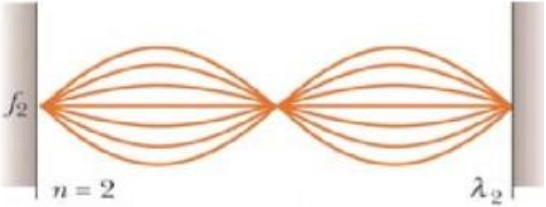
\includegraphics[width=\linewidth, height=30mm]{images/stretched_string_2.jpg}
    \end{minipage}
    & $\lambda_2=L$ & $f_2=\dfrac{v}{\lambda_2}=\dfrac{v}{L}=2f_1$ & 2nd & 1st \\
    \hline
    \begin{minipage}{.3\textwidth}
      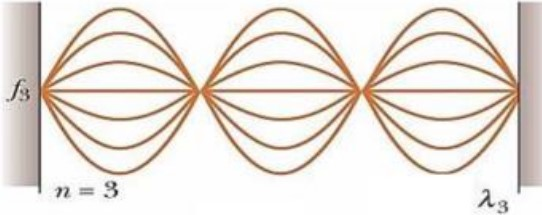
\includegraphics[width=\linewidth, height=30mm]{images/stretched_string_3.jpg}
    \end{minipage}
    & $\lambda_3=\dfrac{2}{3}L$ & $f_3=\dfrac{v}{\lambda_3}=\dfrac{3v}{2L}=3f_1$ & 3rd & 2nd \\
    \hline
  \end{tabular}
\end{table}

Integer number of lops must fit exactly into the length of the string, that is
\[ L=n\brac{\frac{\lambda}{2}} \]

Generalising, the $n$-th harmonic is given by 
\[ f_n = n\brac{\frac{v}{2L}} \]

\subsubsection{Longitudinal stationary waves}

\textbf{Experiment set-up:} Sound wave enters pipe via open end, travels from open end towards closed end, reflected when it hits wall of closed end.  Incident and reflected waves superpose to form a stationary wave.

\textbf{Node}: closed end\footnote{At the nodes, the air particles are not moving. Hence, they allow powder to collect at the nodes.}

\textbf{Antinode}: open end\footnote{At the antinodes, the air particles are moving with maximum amplitude. Hence, they ``push'' the powder away from the antinodes to the nodes.}

\paragraph{Closed pipe}

\paragraph{Open pipe}

\paragraph{End corrections} In practice, antinode at open end occurs \emph{slightly outside} the pipe.

\subsection{Diffraction}
\begin{defn}{Diffraction}{}
\underline{Spreading} of waves at edge of obstacle, or through slit, so that waves do not travel in straight lines.
\end{defn}

\begin{figure}[H]
    \centering
    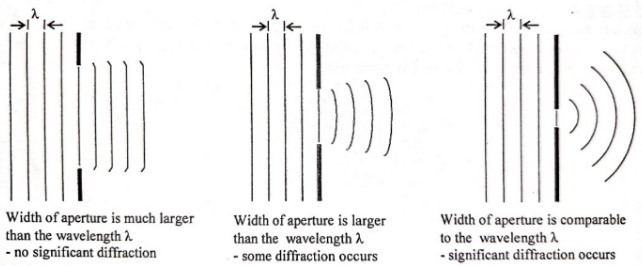
\includegraphics[width=15cm]{images/diffraction_waves.jpg}
\end{figure}

\textbf{Condition}: aperture size (size of slit) is comparable to wavelength (same order), i.e. $b\approx\lambda$.

\subsubsection{Single slit diffraction}
\paragraph{Mimima}
Positions of minima (points of zero intensity) occur at angles
\[ \sin\theta=m\frac{\lambda}{b} \]
where $m=\pm1,\pm2,\dots$

Hence position of first minima is at angle
\begin{equation}
\sin\theta=\frac{\lambda}{b}
\end{equation}

\paragraph{Rayleigh criterion}
Resolution of two objects is the ability to see as distinct two objects that are distinct.

\textbf{Rayleigh criterion} states that for two patterns to be \emph{just resolved}, the central maximum of one must lie on the first minimum of the other.

Minimum angle for two sources to be resolved:
\begin{equation}
\theta\approx\frac{\lambda}{b}
\end{equation}

\subsection{Interference}
\begin{defn}{Coherent waves}{}
Two waves have a \underline{constant phase difference} between them (with respect to time).
\end{defn}

\begin{defn}{Interference}{}
Superposition of \emph{coherent} waves which results in \underline{change in overall intensity}.
\end{defn}

\begin{defn}{Constructive interference}{}
When two waves meet \emph{in phase} at a point, resultant displacement is the \emph{sum} of magnitudes of individual displacements of the two waves.
\end{defn}

Path difference is a whole number of wavelengths, i.e. $n\lambda$.

\begin{defn}{Destructive interference}{}
When two waves meet \emph{antiphase} at a point, resultant displacement is the \emph{difference} of magnitude of individual displacements of the two waves.
\end{defn}

Path difference is an odd number of half wavelengths, i.e. $(n+\frac{1}{2})\lambda$

Conditions for two-source interference fringes to be \emph{observable}:
\begin{enumerate}
\item Waves must \emph{meet}
\item Waves must be \emph{coherent}
\item Waves have (approximately) equal amplitudes
\item Transverse waves must be either unpolarised or polarised in the same plane
\item Split separation is of same order as wavelength, i.e $b\approx\lambda$
\end{enumerate}


\subsubsection{Young's double slit diffraction}

% http://jcphysics.com/wp-content/uploads/2019/03/12-Superposition-Summary.pdf

\begin{equation}
\lambda=\frac{ax}{D}
\end{equation}

\subsection{Diffraction Grating}

\subsection*{Problems}
\begin{prbm}
A sound source of frequency $2500\:\unit{Hz}$ is placed several metres from a plane reflecting wall in a large chamber containing a gas. A microphone, connected to a c.r.o., is used to detect nodes and antinodes formed along the normal from the source to the wall. The microphone is moved from one node through $20$ antinodes to another node, across a distance of $1.90\:\unit{m}$.

Calculate the speed of sound in the gas.
\end{prbm}
\begin{solution}
The sequence of nodes and antinodes are given by
\[ N \quad A \quad N \quad \cdots \quad N \quad A \quad N \]
where the distance between two nodes is $d=\dfrac{\lambda}{2}$.

There are 20 half-wavelengths, so 
\[ 20\brac{\frac{\lambda}{2}}=1.90 \implies \lambda=0.190\:\unit{m} \]
The wavelength of the stationary wave is equal to that of the progressive wave that formed it.

Hence $v=f\lambda=(2500)(0.190)=\boxed{475\:\unit{m\,s^{-1}}}$.
\end{solution}

\pagebreak

\part{Electricity and Magnetism}
\section{Electric Fields}
Types of particles
\begin{itemize}
\item proton: charge $+e$
\item electron: charge $-e$
\item $\alpha$-particle: charge $+2e$
\end{itemize}

\begin{defn}{Coulomb’s Law}{}
Electric force between two \underline{point charges} is proportional to the product of the charges and inversely proportional to the square of their separation.
\begin{equation}
\va{F} = k\frac{Qq}{r^2}\hat{\vb{r}}
\end{equation}
where the constant of proportionality is 
\[ k=\frac{1}{4\pi\epsilon_0} \]
where \textbf{permittivity of free space} $\epsilon_0 = 8.85 \times 10^{-12}\:\unit{F.m^{-1}}$ and can be taken to be equal to that of air unless specified otherwise.
\end{defn}

\begin{remark}
Electric force is repulsive when $Qq>0$ and attractive when $Qq<0$.
\end{remark}

\textbf{Principle of Superposition}: When more than two charges are
present, net force on any one charge is the vector sum of the forces exerted on it by the other charges. For example, if three charges are present, the resultant force experienced by $q_3$ due to $q_1$ and $q_2$ is
\[ \va{F}_3 = \va{F}_{13} + \va{F}_{23} \]
To generalise, for a system of $n$ charges, the net force experienced by the $j$-th particle is
\[ \va{F}_j = \sum_{i=1,i\neq j}^n\va{F}_{ij} \]

\begin{defn}{Electric field}{}
Region of space where a charge experiences an electric force.
\end{defn}

Representation of electric field using \textbf{field lines} (lines of force):
\begin{itemize}
\item An electric field line indicates the direction of the force a positive charge would experience if it is placed at that point in the field (at a normal to surface of charge).
\item The number of field lines per unit cross-sectional area is proportional to the \textbf{electric field strength}.
\item Electric field lines are directed away from positive to negative charges, never intersect each other, and are never created or annihilated in vacuum.
\end{itemize}

\begin{defn}{Electric field strength $\va{E}$}{}
Electric force per unit positive charge on a \emph{small test charge} placed at that point.
\begin{equation} \va{E}=\frac{F}{q}=k\frac{Q}{r^2} \end{equation}
\end{defn}

\begin{remark}
We take charge $q$ to be infinitesimally small so that the field it generates does not disturb that of the ``source charge'', i.e. charge $Q$.
\end{remark}

Comparison between electric field and gravitational field:
\begin{itemize}
\item Qualitative aspect: Gravitational force results from interaction between masses; electric force results from interaction between charges.
\item Quantative aspect: Both fields are inverse square law fields.
\end{itemize}

\begin{defn}{Electric potential $V$}{}
Work done per unit positive charge by an external force in bringing a \emph{small test charge} from infinity to that point.
\begin{equation} V=\frac{W}{q}=k\frac{Q}{r} \end{equation}
where $W$ is the work done on the charge.
\end{defn}

Positive charges move from places of high potential to lower potential, EPE increases.

Negative charges move from places of low potential to higher potential, EPE decreases.

\begin{defn}{Electric potential energy $U$}{}
When two point charges $Q$ and $q$ are at a distance $r$ apart, electric potential energy $U$ of the \emph{system of two charges} is given by 
\begin{equation} U=qV=k\frac{Qq}{r} \end{equation}
\end{defn}

\begin{remark}
EPE can be negative, if one charge is positive and the other is negative.
\end{remark}

\subsection{Parallel plates}
\begin{figure}[H]
    \centering
    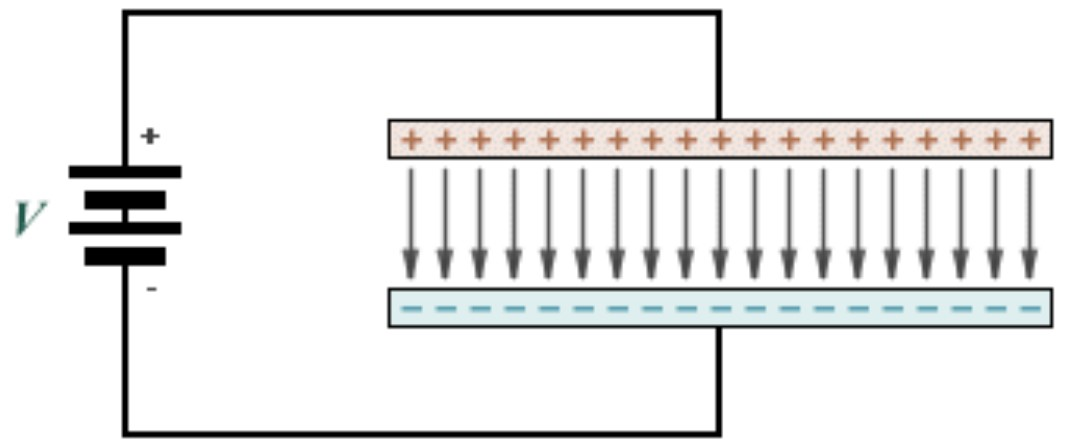
\includegraphics[width=8cm]{images/parallel_plates.jpg}
\end{figure}

Electric field set up is uniform, hence electric field strength $E$ is constant. Thus $F=qE$.

\begin{equation}
E = \frac{|\Delta V|}{d}
\end{equation}
where $|\Delta V|$ is the potential difference across the plates, $d$ is the separation of the plates.

\subsubsection{Charge Moving Perpendicularly to an Electric Field}
\begin{figure}[H]
    \centering
    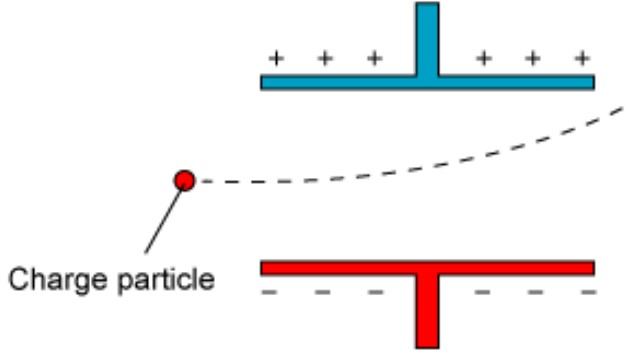
\includegraphics[width=8cm]{images/parallelplates_parabolic.jpg}
\end{figure}

Motion of charged particle in electric field is \textbf{parabolic} in nature.

\begin{proof}
By Newton's 2nd Law, acceleration is given by
\[ a=\frac{F}{m} = \frac{qE}{m} = \frac{q|\Delta V|}{md} \]
which is constant.

Assuming particle is initially at rest, then velocity is given by 
\[ v = u+at = \frac{qE}{m}t \]

When the particle projection is perpendicular to the direction of the electric field, then motion is in the upward direction (along $y$-axis). Thus displacement in $y$-direction is 
\[ y = ut+\frac{1}{2}at^2 = \frac{qE}{2m}t^2 \]

Since $v=xt$, eliminating time dependence gives us 
\[ y = \frac{qE}{2mv^2}x^2 \]
The $y$-$x$ relation is a parabola. Hence the particle follows a parabolic trajectory.
\end{proof}

\subsubsection{Millikan's oil drop}
Physicist Robert Millikan's experiment involves spraying tiny oil droplets into a vertical chamber with two metal plates on either end. The oil droplets became charged. When they entered the chamber, they began to fall under the influence of gravity. He then stopped the free-falling droplets and reversed their direction of motion by applying a voltage across the two metal plates. 

He measured the velocity of a single oil droplet in the electric field to determine the electrical force $F$ acting on it. This allowed him to determine the charge on the oil droplet, since $q=\frac{F}{E}$.

\begin{figure}[H]
    \centering
    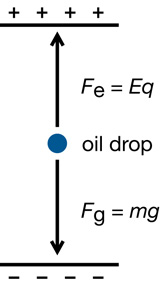
\includegraphics[width=3cm]{images/oil-droplet_free_body_diagram.jpg}
\end{figure}

By measuring the charge of many droplets and comparing them, he reasoned that the smallest difference in charge among all the droplets would be due to the presence of one extra electron. That small difference in charge would then be equal to the charge of a single electron or the elementary charge. He then discovered that the charges of the oil droplets were always integer multiples of $1.60 \times 10^{-19}\:\unit{C}$. He reasoned this must be the charge of a single electron, a value that is referred to as the \textbf{elementary unit of charge}.

% https://www.lancaster.ac.uk/media/lancaster-university/content-assets/images/physics/lab-in-a-box/LabInABox_Milikans.pdf
\pagebreak

\subsection*{Problems}
\begin{prbm}
Josiah bought a small engagement ring of mass $m = 1.00 \times 10^{-3}\:\unit{kg}$, which he wanted to present to his fianc\'{e}e in a box with a square base of side length $s=0.100\:\unit{m}$ and negligible height. On opening the box, he wanted the ring to hover a short distance above its centre. To achieve this, he hid a positive point charge $+q$ under the centre of the box and applied the same positive charge $+q$ to the ring. To constrain the ring to hover directly above the centre of the box, he tied four thin inextensible strings of length $l=0.120\:\unit{m}$ to the ring and secured them to the four corners of the box. 

Suppose the ring is small enough to be approximated by a point charge. What is the minimum charge $q$ required to ensure the four strings remain taut while the ring hovers above the box?

\textit{Leave your answer to 3 significant figures in units of $\mu\:\unit{C}$.}

\begin{figure}[H]
    \centering
    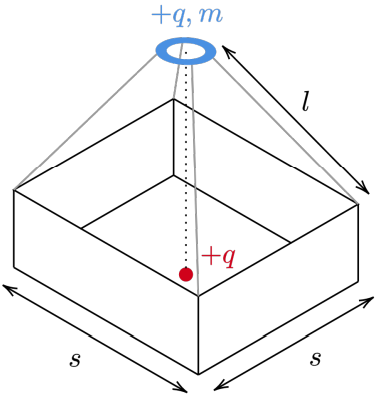
\includegraphics[width=6cm]{images/A_Simple_Proposal.png}
\end{figure}
\end{prbm}

\begin{solution}
Three types of forces act on the hovering ring: the electrostatic repulsion from the hidden point charge, the weight of the ring, and the tension from the strings. These forces must cancel for the ring to hover in place.

Let $h$ be the height above the box at which the ring hovers, and let us define the downwards direction to be positive. As shown in the diagram, the electrostatic repulsion is $-\dfrac{q^2}{4\pi\epsilon_0h^2}$ while the weight from the ring is $+mg$.

Since the net (downwards) force from the tension of the four strings, T, balances the gravitational and electrostatic forces on the ring, we have:
\[ T=\frac{q^2}{4\pi\epsilon_0h^2}-mg \]

\begin{figure}[H]
    \centering
    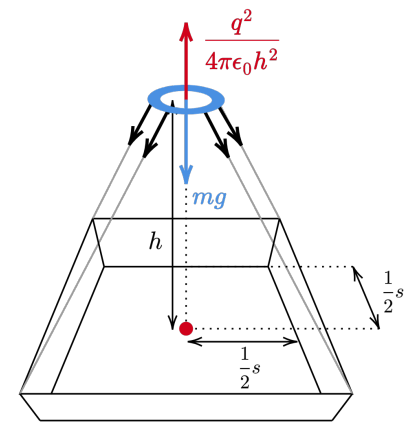
\includegraphics[width=8cm]{images/A_Simple_Proposal1.png}
\end{figure}

For the strings to remain taut, the tensions in the string must be non-negative, which implies that:
\[ T=\frac{q^2}{4\pi\epsilon_0h^2}-mg\ge0 \implies q^2\ge4\pi\epsilon_0mgh^2 \]
From the same diagram above and Pythagoras’s theorem, we can infer that:
\[ l^2=\brac{\frac{s}{2}}^2+\brac{\frac{s}{2}}^2+h^2 \implies h=\sqrt{l^2-\frac{s^2}{2}} \]

Substituting this expression for $h$ into the previous equation and isolating $q$ implies that the charge must be at least:
\begin{align*}
q &\ge \sqrt{4\pi\epsilon_0mg\brac{l^2-\frac{s^2}{2}}} \\
\Aboxed{q &\approx 0.101\:\mu\unit{C}}
\end{align*}
\end{solution}

\pagebreak
\section{Current of Electricity}
\subsection{Electric current}
\textbf{Elementary charge}:
\[ e = 1.6 \times 10^{-19}\:\unit{C} \]
\begin{itemize}
\item Protons are positively charged, with a charge $+e$.
\item Electrons are negatively charged, with a charge $-e$. 
\item Ions carry charges that are multiples of $+e$ and $-e$.
\end{itemize}

\begin{defn}{Electric current $I$}{}
Rate of flow of charge.
\[ I=\odv{Q}{t} \]
For a steady current $I$, we have 
\begin{equation}
Q = It
\end{equation}
\end{defn}

\begin{remark}
By convention, the direction of current is the direction that \underline{positive charges} move. However, remember that current is due to the flow of \underline{electrons}; lattice atoms/ions do not move.
\end{remark}

\textbf{Transport equation}:
\begin{equation}
I=nAvq
\end{equation}
where $v$ is the \textbf{drift velocity}.

\begin{figure}[H]
    \centering
    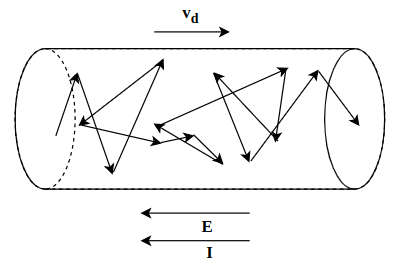
\includegraphics[width=8cm]{images/transport_eqn.png}
\end{figure}

\begin{remark}
Drift velocity of charge carriers is much lower than the maximum velocity that charge carriers could achieve from the potential difference applied to the wire.

This is because charge carriers experience electrical force in \underline{all directions} because of collisions with lattice ions. This produces a range of velocities. The drift velocity is an \underline{average}.
\end{remark}

\begin{remark}
When a domestic lighting circuit is switched on, the lights come on almost immediately. 
This is because when the switch is on, all electrons in the wire and filament start to move \underline{together}.
\end{remark}
\pagebreak

\subsection{Potential difference and electromotive force}
\begin{defn}{Potential difference $V$}{}
\underline{Work done per unit charge} when electrical energy is converted into non-electrical energy when the charge passes \underline{from one point to the other}.
\begin{equation}
V = \frac{W}{Q}
\end{equation}
\end{defn}

\begin{defn}{Electromotive force $\epsilon$}{}
\underline{Work done per unit charge} when non-electrical energy is converted into electrical energy when the charge is moved \underline{around a complete circuit}.
\begin{equation}
\epsilon = \frac{W}{Q}
\end{equation}
\end{defn}

\begin{table}[H]
\centering
\begin{tabular}{|p{7.5cm}|p{7.5cm}|}
\hline
\textbf{Potential difference} & \textbf{Electromotive force} \\
\hline
Refers only to source & Refers to any two points in the circuit \\
Amount of non-electrical energy converted into electrical energy & Amount of electrical energy into non-electrical energy \\
Always exists as it is a source of energy & Only exists if current is flowing \\
\hline
\end{tabular}
\end{table}

\begin{figure}[H]
    \centering
    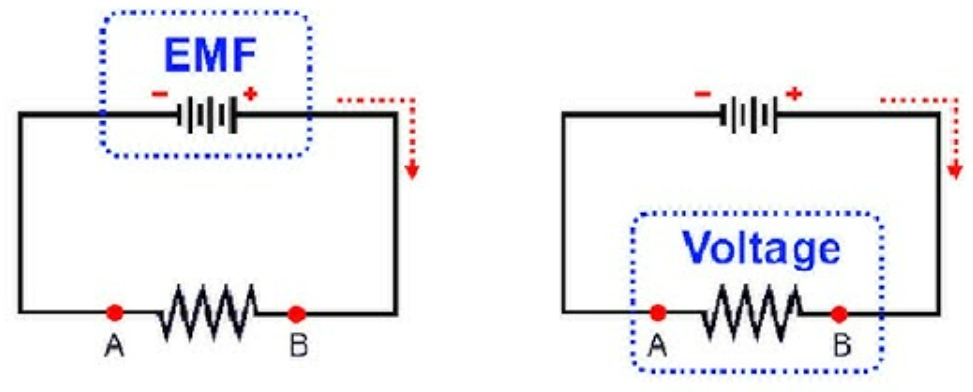
\includegraphics[width=10cm]{images/pd_emf.png}
\end{figure}
\pagebreak

\subsection{Resistance}
\begin{defn}{Resistance $R$}{}
\underline{Ratio} of potential difference across component to current flowing through it.
\begin{equation}
R = \frac{V}{I}
\end{equation}
\end{defn}

\textbf{Resistivity} is a property unique to the material.
\begin{equation}
R = \rho \frac{l}{A}
\end{equation}

\begin{defn}{Ohm's Law}{}
Current flowing through conductor is directly proportional to potential difference applied across it, provided that \underline{physical conditions remain constant}.
\begin{equation}
I \propto V
\end{equation}
\end{defn}
\pagebreak

\subsection{I-V characteristics}
An ohmic resistor obeys Ohm's Law. For non-ohmic resistors that do not obey Ohm's Law, factors that cause resistance to deviate are:
\begin{enumerate}
\item Number density of charge carriers $n$ (decrease resistance)
\item Amplitude of atomic vibrations of lattice atoms (increase resistance)
\end{enumerate}

\subsubsection{Ohmic resistor}

\begin{figure}[H]
\centering
\begin{tikzpicture}
  \begin{axis}%
    [axis lines=middle,
     enlargelimits={abs=0.2},
     xlabel = $V$,
     ylabel = $I$,
     ticks=none
    ]
    \addplot[domain=-2:2,samples=50,smooth,red] {x};
  \end{axis}
\end{tikzpicture}
\end{figure}

Resistance is \textbf{constant}: as p.d. increases, current increases proportionately.

\subsubsection{Filament lamp}

\begin{figure}[H]
\centering
\begin{tikzpicture}
  \begin{axis}%
    [axis lines=middle,
     enlargelimits={abs=0.2},
     xlabel = $V$,
     ylabel = $I$,
     ticks=none
    ]
    \addplot[domain=-1.57:1.57,samples=50,smooth,red] {sin(deg(x))};
  \end{axis}
\end{tikzpicture}
\end{figure}

Resistance \textbf{increases}: as p.d. increases, current increases less than proportionately.

\begin{tcolorbox}
\textbf{Alternative explanation:}

The gradient of the line joining the origin to each point on the curve decreases as p.d. increases.

Since resistance is the reciprocal of the gradient, resistance increases as p.d. increases.
\end{tcolorbox}

\begin{itemize}
\item \underline{As temperature increases}, amplitude of atomic vibrations of lattice atoms increases.
\item $n$ does not increase significantly. 
\item Overall effect is resistance increases.
\end{itemize}

\textbf{Useful problem solving technique:}

To find a particular resistance value on an $I-V$ graph, draw the $I-V$ graph of an ohmic conductor with the particular resistance value.

\subsubsection{Semiconductor diode}

\begin{tcolorbox}
\textbf{What is a semiconductor diode?}

A diode is a two-terminal electronic component that has a \underline{low resistance} to the flow of current in one direction thus allowing the passage of current in one direction (\textbf{forward bias}) whereas there will be a \underline{high resistance} in the other, thus restricting the flow of current in that direction (\textbf{reverse bias}).
\end{tcolorbox}

\begin{figure}[H]
\centering
\begin{tikzpicture}
  \begin{axis}%
    [axis lines=middle,
     enlargelimits={abs=0.2},
     xlabel = $V$,
     ylabel = $I$,
     ticks=none
    ]
    \addplot[domain=0:5,samples=50,smooth,red] {x^3};
    \addplot[domain=-2:0,samples=50,smooth,red] {0.0};
    \addplot[domain=-4.5:-2,samples=50,smooth,red] {(x+2)^5};
  \end{axis}
\end{tikzpicture}
\end{figure}

For forward-biased region, resistance \textbf{decreases}: as p.d. increases, current increases more than proportionately.

\begin{itemize}
\item \underline{As temperature increases}, electrons in semiconductor are more likely to have sufficient energy to escape from atom, so $n$ increases significantly.
\item Increase in rate of interaction of electrons with vibrating atoms.
\item Increase in $n$ \underline{predominates over} increase in rate of interactions of electrons with lattice. Overall effect is resistance decreases.
\end{itemize}

For reverse-biased region, resistance is \textbf{infinitely high}: no current flow through diode until breakdown voltage.
\pagebreak

\subsubsection{Negative Temperature Coefficient (NTC) thermistor}

\begin{figure}[H]
\centering
\begin{tikzpicture}
  \begin{axis}%
    [axis lines=middle,
     enlargelimits={abs=0.2},
     xlabel = $V$,
     ylabel = $I$,
     ticks=none
    ]
    \addplot[domain=-2:2,samples=50,smooth,red] {x^3};
  \end{axis}
\end{tikzpicture}
\end{figure}

Resistance \textbf{decreases}: as p.d. increases, current increases more than proportionately.

\begin{itemize}
\item \underline{As temperature increases}, electrons are more likely to have sufficient energy to escape from atom, so $n$ increases significantly.
\item Increase in rate of interaction of electrons with vibrating atoms.
\item Increase in $n$ \underline{predominates over} rate of interactions of electrons with lattice. Overall effect is resistance decreases.
\end{itemize}

\begin{remark}
As temperature of thermistor increases, its resistance decreases.

Since e.m.f. of battery remains unchanged, current increases when resistance decreases, causing greater power to be generated in the thermistor.

This will result in a further increase in temperature of thermistor, decrease in its resistance, leading to \textbf{thermal runaway} which could cause overheating.
\end{remark}

Resistance-temperature characteristic: resistance decreases as temperature increases

\begin{figure}[H]
\centering
\begin{tikzpicture}
  \begin{axis}%
    [axis lines=middle,
     enlargelimits={abs=0.2},
     xlabel = $T$,
     ylabel = $R$,
     ticks=none
    ]
    \addplot[domain=0:5,samples=50,smooth,red] {1/x};
  \end{axis}
\end{tikzpicture}
\end{figure}

\subsubsection{Light Dependent Resistor (LDR)}
Similar to NTC thermistor.
\pagebreak

\subsection{Power}
Electrical power dissipated by the conductor:
\begin{equation}
\begin{split}
P &= VI \\
P &= I^2R \\
P &= \frac{V^2}{R}
\end{split}
\end{equation}

\subsection{Internal resistance}
Let $r$ denote internal resistance of battery, $R$ denote resistance of load, $V$ denote terminal p.d. of battery, $\epsilon$ denote e.m.f.

For an \textbf{ideal} battery, $r=0$. This gives us 
\[ \epsilon=V \]

For a \textbf{real} battery, $r\neq 0$. We imagine the internal resistance as another load of resistance $r$ connected with $R$ in series. 

\begin{figure}[H]
    \centering
    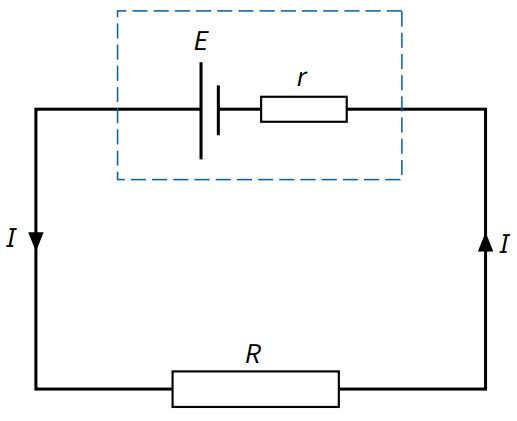
\includegraphics[width=8cm]{images/internal_resistance.jpg}
\end{figure}

Since e.m.f. is sum of p.d., 
\[ \epsilon=I(R+r) \]
\begin{equation}
\epsilon=V+Ir
\end{equation}

This gives us
\[ \boxed{I=\frac{\epsilon}{R+r}} \]

\pagebreak

\subsection*{Problems}
\begin{prbm}
The terminals of a battery are connected to a load resistance. As the battery increases, its internal resistance increases. How does this affect the ability of the battery to deliver energy?
\end{prbm}

\begin{proof}[Answer]
Terminal p.d. decreases. Power delivered to the load decreases (p.d. decrease, resistance constant) as more energy dissipated as heat by internal resistance of battery.
\end{proof}

\begin{prbm}
By considering a practical source with e.m.f. $E$ and internal resistance $r$ connected in series with an electrical device of resistance $R$, determine
\begin{enumerate}[label=(\roman*)]
\item an expression for output efficiency of the source, $\eta=\dfrac{\text{useful power output}}{\text{total power generated}}$.
\item the value of $R$ in terms of $r$ such that maximum power is delivered to the device, and the output efficiency of the source when it is used to operate an electrical device at maximum power.
\end{enumerate}
\end{prbm}

\begin{proof}[Answer] \
\begin{enumerate}[label=(\roman*)]
\item Total power generated:
\[ P_{gen}=I^2(R+r) \]

Useful power output:
\[ P_{out}=I^2R \]

Efficiency:
\[ \boxed{\eta = \frac{R}{R+r}} \]

\item Current in the circuit:
\[ I = \frac{E}{R+r} \]

Power output at the load:
\[ P_{out} = I^2R = \brac{\frac{E}{R+r}}^2R \]

For maximum power output,
\[ \dv{P_{out}}{R} = 0 \implies \boxed{R=r} \]

Output efficiency is \boxed{0.5} (50\%).
\end{enumerate}
\end{proof}
\pagebreak
\section{D.C. Circuits}
\textbf{Direct current} (d.c.): current flowing only in \emph{one direction}

\subsection{Circuit symbols and diagrams}
Circuit symbols:

\begin{figure}[H]
    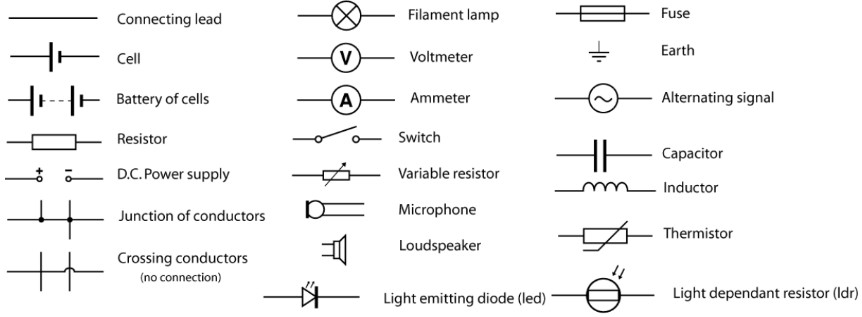
\includegraphics[width=16cm]{images/circuit_symbols.jpg}
\end{figure}

\subsection{Series and parallel arrangements}
\subsubsection{Current}
Current divides up where a circuit splits into multiple branches. 
\begin{defn}{Kirchhoff’s Current Law}{}
Algebraic sum of the currents at a junction of a circuit is zero.
\begin{equation}
\sum_{\text{junction}}I_i=0
\end{equation}
Currents entering the junction are given a positive $(+)$ sign, currents leaving the junction are given a negative $(-)$ sign.
\end{defn}

This means sum of currents entering a junction = sum of currents leaving the junction
\[ \sum I_\text{in} = \sum I_\text{out} \]

\begin{proof}
By the Principle of Conservation of Charge, the total charge that enters a junction per unit time must be equal to the total charge that leaves the same junction per unit time.
\end{proof}

\paragraph{Series}
Currents at all points are same, equal to total current.
\[ I_1=\cdots=I_n=I \]

\paragraph{Parallel}
Total current is sum of individual currents.
\[ I = I_1+\cdots+I_n \]

\subsubsection{Voltage}
\begin{defn}{Kirchhoff’s Voltage Law}{}
Algebraic sum of all electrical potential changes around any closed loop is zero.
\begin{equation}
\sum_{\text{junction}}\Delta V_i=0
\end{equation}
\end{defn}

This means the sum of the e.m.f.s around any loop in a circuit is equal to the sum of the p.d.s around the loop.
\[ \sum \epsilon = \sum V_\text{drop} \]

\begin{proof}
By the Law of Conservation of Energy, energy supplied by the source is equal to energy dissipated by resistors.

For constant current and time,
\begin{align*}
\brac{I\sum\epsilon}t &= \brac{I^2\sum R}t \\
\sum\epsilon &= I\sum R \\
\sum\epsilon &= \sum V
\end{align*}
\end{proof}

\begin{remark}
Current always flows from higher potential to lower potential.
\end{remark}

\paragraph{Series}
e.m.f. is sum of voltages.
\[ V_1+\cdots+V_n = \epsilon \]

\paragraph{Parallel}
Voltages are same, equal to e.m.f.
\[ \epsilon = V_1=\cdots=V_n \]

\subsubsection{Resistance}
\paragraph{Series}
Effective resistance is sum of individual resistances

\begin{equation}
R_{\text{eff}} = R_1 + \cdots + R_n
\end{equation}

\begin{derivation}
Consider two resistors of resistances $R_1$ and $R_2$ connected in series. 

According to Kirchhoff’s current law, the current in each resistor is the same. The p.d. $V$ across the combination is equal to the sum of the p.d.s across the two resistors:
\[ V = V_1+V_2 \]
Since $V = IR$, $V_1 = IR_1$ and $V_2 = IR_2$, we can write:
\[ IR = IR_1+IR_2 \]
Cancelling the common factor of current $I$ gives:
\[ R = R_1+R_2 \]
For three or more resistors, the equation for total resistance $R$ becomes:
\[ R = R_1+R_2+R_3+\cdots \]
\end{derivation}

\paragraph{Parallel}
Reciprocal of effective resistance is sum of reciprocals of individual resistances

\begin{equation}
\frac{1}{R_\text{eff}} = \frac{1}{R_1} + \cdots + \frac{1}{R_n}
\end{equation}

\begin{remark}
Effective resistance of resistors in parallel is always lower than the lowest resistance in the network.
\end{remark}

\begin{derivation}
Consider two resistors of resistances $R_1$ and $R_2$ connected in parallel. The total current is divided between them. 

Using Kirchhoff's current law,
\[ I = I_1+I_2 \]
Applying Kirchhoff's voltage law to the loop that contains the two resistors,
\[ I_1R_1 - I_2R_2 = 0 \]
(because there is no source of e.m.f. in the loop)

This suggests that the two resistors have the same p.d. across them. Hence we can write $I=\frac{V}{R}$, $I_1=\frac{V_1}{R_1}$ and $I_2=\frac{V_2}{R_2}$.

Substituting these into $I = I_1+I_2$ and cancelling the common factor $V$,
\[ \frac{1}{R} = \frac{1}{R_1} + \frac{1}{R_2} \]

For three or more resistors, the equation for total resistance $R$ becomes
\[ \frac{1}{R} = \frac{1}{R_1} + \frac{1}{R_2} + \frac{1}{R_3} + \cdots \]
\end{derivation}

\subsubsection{Measuring instruments}
\begin{table}[H]
\centering
\begin{tabular}{|c|c|c|c|}
\hline
\textbf{Instrument} & \textbf{Measured quantity} & \textbf{Assumption}\footnote{unless stated otherwise} & \textbf{Connection} \\
\hline
\textbf{ammeter} & current (in one direction) & zero (internal) resistance & in series \\
\textbf{galvanometer} & current (in both directions) & zero (internal) resistance & in series \\
\textbf{voltmeter} & potential difference & infinite resistance & in parallel \\
\hline
\end{tabular}
\end{table}

\subsection{Potential divider}
\begin{defn}{Potential divider rule}{}
If a voltage exists across several resistors connected in series, then the voltage across each resistor is proportional to the total resistance.
\begin{equation}
V_1 = \frac{R_1}{R_T}V
\end{equation}
\end{defn}

\begin{derivation}
Consider two resistors $R_1$ and $R_2$ are connected in \emph{series}. The \emph{same} current flows through both resistors.

Hence p.d. across $R_1$ is given by
\[ V_1 = IR_1 = \brac{\frac{E}{R_1+R_2}}R_1 = \brac{\frac{R_1}{R_1+R_2}}E \]
or
\[ \frac{V_1}{E} = \frac{R_1}{R_T} \]
This means that the two resistors divide the total p.d. into fractions according to their resistance.
\end{derivation}

Using the potential-divider principle for a continuous resistor (e.g. a resistance wire) which has constant resistance per unit length, the voltage drop across a section of the wire $AB$ is proportional to the length of $AB$ as a fraction to the wire's total length.
\[ V_{AB} = \frac{\ell_{AB}}{\ell_T} \times V \]

\begin{tcolorbox}
Consider a wire of non-uniform resistance per unit length, who resistance is described by the function $R(x)$. Integrating over the length of the wire $L$ gives the total resistance of the wire:
\[ R = \int_0^L R(x) \dd{x} \]
where the length $x$ is measured from one fixed end of the wire.
\end{tcolorbox}

\subsubsection{Potentiometer}
A \vocab{potentiometer} is a device used for comparing potential differences \emph{without drawing a current}\footnote{This is in contrast to a voltmeter. A non--ideal voltmeter draws some current from the circuit as it does not have infinitely high resistance.} from the circuit involved. It is used to measure the unknown e.m.f. of a source $E_1$, using another source of known e.m.f. $E_0$.

\begin{figure}[H]
    \centering
    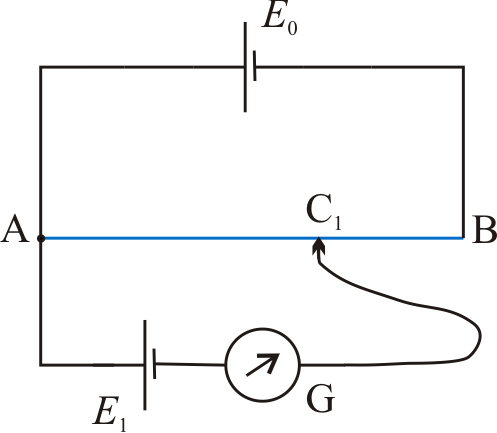
\includegraphics[width=6cm]{images/potentiometer.png}
\end{figure}

\begin{proposition}
Along the slide wire, $V \propto \ell$.
\end{proposition}
\begin{proof}
p.d. across $AB$ is
\[ V_{AB} = IR_{AB} = I\brac{\frac{\rho\ell_{AB}}{A}} \]
Similarly, p.d. across $AY$ is
\[ V_{AC} = IR_{AC} = I\brac{\frac{\rho\ell_{AC}}{A}} \]
Hence it is evident that 
\[ \frac{V_{AC}}{V_{AB}} = \frac{\ell_{AC}}{\ell_{AB}} \implies \boxed{V \propto \ell} \]
\end{proof}

\begin{remark}
Recall that there needs to be a potential difference for current to flow.
\end{remark}

\textbf{Objective:} Locate the \textbf{balance point} to determine \textbf{balance length}.
\begin{itemize}
\item At the balance point, No current flows through galvanometer. Galvanometer registers zero reading.
\item This means no potential difference between point $A$ and $+$ve terminal of $E_1$, and between point $C$ and $-$ve terminal of $E_1$. Hence p.d. between $A$ and $C$ is equal to p.d. across $E_1$, thus $E_1=V_{AC}$.
\item Since p.d. is proportional to length across slide wire, we have 
\[ E_1 = V_{AC} = \frac{\ell_{AC}}{\ell_{AB}}V_{AB} \]
\end{itemize}

\subsubsection{Wheatstone bridge}
The Wheatstone bridge is a way to measure the resistance of unknown resistors placed in the position of $R_4$, where the resistance of variable resistor $R_3$ is adjustable.

\begin{figure}[H]
    \centering
    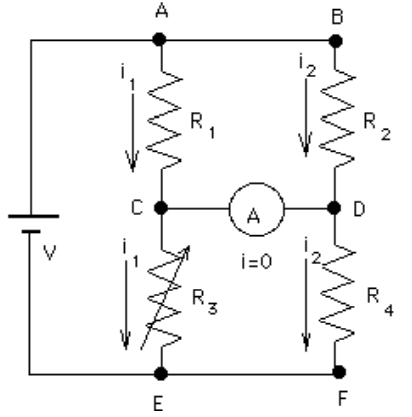
\includegraphics[width=8cm]{images/wheatstone.png}
\end{figure}

Since no current flows in the ammeter, no potential difference between points $C$ and $D$. Hence $V_C=V_D$.

Since no current flows through the ammeter, $I_1=I_3$ and $I_2=I_4$. It also follows (from the fact that points C and D have the same potential) that the voltage drop across $R_1$ is the same as the voltage drop across resistor $R_2$. Hence
\begin{equation*}\tag{1}
I_1 R_1 = I_2 R_2
\end{equation*}

Similarly, voltage drop across $R_3$ is the same as voltage drop across $R_4$ so
\begin{equation*}\tag{2}
I_1 R_3 = I_2 R_4
\end{equation*}

Dividing (1) by (2) gives us
\begin{equation*}\tag{3}
\frac{R_1}{R_3} = \frac{R_2}{R_4}
\end{equation*}

Solving (3) for the unknown resistor $R_4$,
\[ R_4 = \frac{R_2}{R_1}R_3 \]
\pagebreak

\subsection*{Problems}
\begin{prbm}[M\"{o}bius Strip]
Two wires are each strung with 4 resistors, along with another 4 resistors that bridge pairs of resistors across both wires. The wires are then twisted together to form a M\"{o}bius strip, as shown below.

\begin{figure}[H]
    \centering
    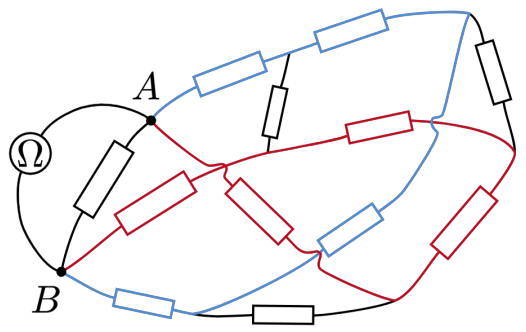
\includegraphics[width=7cm]{images/Mobius_strip.png}
\end{figure}

Every resistor has identical resistance $R = 1.0\:\Omega$. Determine the equivalent resistance $R_{eq}$ between the points $A$ and $B$ in the M\"{o}bius strip.

\textit{Leave your answer to 2 significant figures in units of $\Omega$.}
\end{prbm}

\begin{solution}
Imagine ``slicing" the M\"{o}bius strip along line AB and then opening up and untwisting the circuit. The circuit can then be redrawn in its deconstructed form:

\begin{figure}[H]
    \centering
    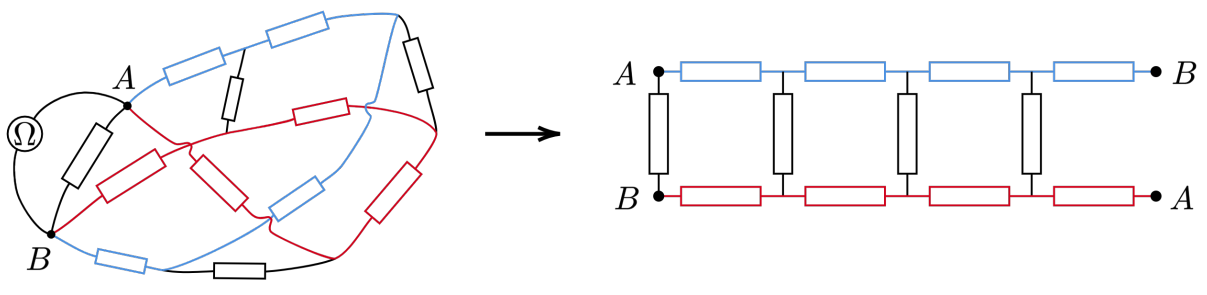
\includegraphics[width=15cm]{images/Mobius_strip_1.png}
\end{figure}

To determine the resistance $R_{eq}$ across $AB$, we can treat the 1 bridging resistor, of resistance $R$, to be in parallel with the rest of the circuit, of unknown resistance $R^\prime$.

\begin{figure}[H]
    \centering
    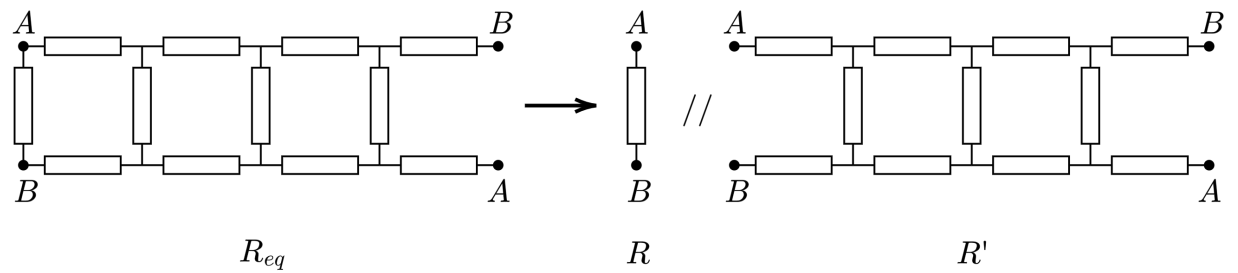
\includegraphics[width=15cm]{images/Mobius_strip_2.png}
\end{figure}

Let us now focus on finding this unknown resistance $R^\prime$. Notice that due to the symmetry of this circuit, there are 3 pairs of equipotential points as marked below (each pair takes a different colour). As such, we obtain the following equivalent circuit after combining points $A$ and $B$ on both ends:

\begin{figure}[H]
    \centering
    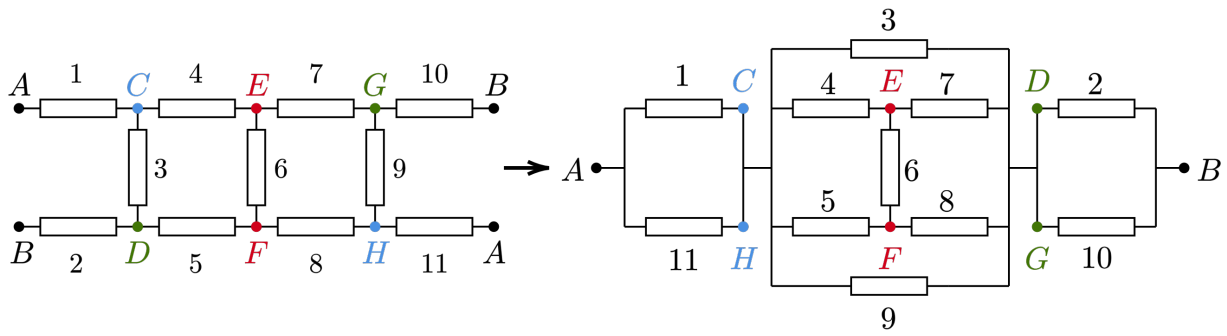
\includegraphics[width=15cm]{images/Mobius_strip_3.png}
\end{figure}

From here, we can determine the value of $R^\prime$ (noting that resistor 6 can be disregarded since its two ends are equipotential):

\[ R^\prime = \frac{1}{\frac{1}{R}+\frac{1}{R}} + \frac{1}{\frac{1}{R}+\frac{1}{2R}+\frac{1}{2R}+\frac{1}{R}} + \frac{1}{\frac{1}{R}+\frac{1}{R}} = \frac{4}{3}R \]

We can hence calculate the resistance $R_{eq}$ of the complete circuit:

\[ R_{eq} = \frac{1}{\frac{1}{R}+\frac{1}{R^\prime}} = \frac{4}{7}R \approx \boxed{0.57\:\Omega} \]
\end{solution}
\pagebreak

\begin{prbm}[Hexagonmania]
Roger is bored, so he decides to use his collection of uniform thin copper rods, each of resistance $R = 1.00\:\Omega$, to create a rigid compound shape shown below. The copper rods form seven regular hexagons. Calculate the effective resistance $R_{AB}$ between points $A$ and $B$.

\textit{Leave your answer to 3 significant figures in units of $\Omega$.}
\end{prbm}

\begin{solution}
% https://sgphysicsleague.org/archives/2023/solutions.pdf Problem 38
\end{solution}
\pagebreak
\section{Electromagnetism}
\subsection{Concept of a magnetic field}
\textbf{Magnets} produce magnetic fields. 
\begin{itemize}
\item Hard magnetic materials like cobalt and nickel are difficult to magnetise but tend to retain their magnetism.
\item Soft magnetic materials like iron are easily magnetised but tend to lose their magnetism easily.
\end{itemize}

\begin{defn}{Magnetic field}{}
Region of space where a magnetic pole, a current-carrying conductor or a moving charge particle will experience a force.
\end{defn}

A magnetic field can be produced by:
\begin{enumerate}
\item permanent magnets
\item current-carrying conductors
\end{enumerate}

\subsubsection{Magnetic field lines}
\begin{itemize}
\item The field is represented by lines of force, starting from the North pole and ending at the South pole.
\item The tangent to the magnetic field line at a point in the magnetic field gives the direction of the field at that point.
\item The number of lines per unit cross section area is an indication of the strength of the field.
\end{itemize}

Magnetic field strength at a point is denoted by $B$.

Arrow: Magnetic field acting in direction of arrow

Cross: Magnetic field acting into plane of paper

Dot with a circle: Magnetic field acting out of the plane of paper

Use right hand rule to determine direction of magnetic field due to current.

\subsubsection{Magnetic Flux Patterns}
\paragraph{Due to current in long straight wire}
magnetic flux density $B$:
\begin{equation}
B = \frac{\mu_0I}{2\pi r}
\end{equation}
where $\mu_0$ is the vacuum magnetic permeability constant.

\paragraph{Due to current in flat circular coil}
magnetic flux density $B$:
\begin{equation}
B = \frac{\mu_0 NI}{2r}
\end{equation}

\paragraph{Due to current in long solenoid}
magnetic flux density $B$:
\begin{equation}
B = \mu_0 nI
\end{equation}

\subsection{Magnetic force}
\subsubsection{Force on a current-carrying conductor}
Direction of the force can be determined using Fleming’s left hand rule. 

Magnitude of the force:
\begin{equation}
F = BIL\sin\theta
\end{equation}
where $\theta$ is the angle between the magnetic field vector and the direction of the current.

In vector form:
\[ \vb{F} = \vb{IL} \times \vb{B} \]

\begin{defn}{Magnetic flux density $B$}{}
Force acting per unit length of a conductor which carries unit current and is of right angles to the magnetic field.
\[ B = \frac{F}{IL\sin\theta} \]
\textbf{Tesla} is the unit of magnetic flux density equivalent to a force of 1 \unit{N} experienced by a straight conductor of length 1 \unit{m} and carrying a current of 1 \unit{A} when it is placed perpendicular to the magnetic field.
\end{defn}

\subsubsection{Force between current-carrying conductors}
Currents in same direction: attract each other

Currents in opposite direction: repel each other

Force of interaction:
\[ F \propto \frac{I_1I_2}{d} \]
\begin{equation}
F_1 = BI_1L = \frac{\mu_0I_2}{2\pi r}I_1L
\end{equation}

\subsubsection{Force on a moving charge}
As current consists of moving charges, it can be deduced that a moving charged particle also experiences an electromagnetic force. Consider a charge $q$ travelling at constant speed $v$ at an angle $\theta$ to magnetic field of flux density $B$.

Assume the charge travels a distance in time $t$, so $v=\dfrac{L}{t}$ thus $L=vt$.

Equation for force on conductor $F=BIL\sin\theta$ can be rearranged as
\[ F = B\brac{\frac{q}{t}}(vt)\sin\theta \]
\begin{equation}
F = Bqv\sin\theta
\end{equation}

\subsubsection{Circulating Charge}
If $v$ and $B$ are \emph{perpendicular}, force will make the charge undergo \underline{uniform circular motion}.

\textbf{Magnetic force provides centripetal force}:
\[ F_B = F_c \implies Bqv = \frac{mv^2}{r} \implies \boxed{r=\frac{mv}{Bq}} \]
This means that for larger $v$, $r$ is larger, and vice versa.

\begin{figure}[H]
    \centering
    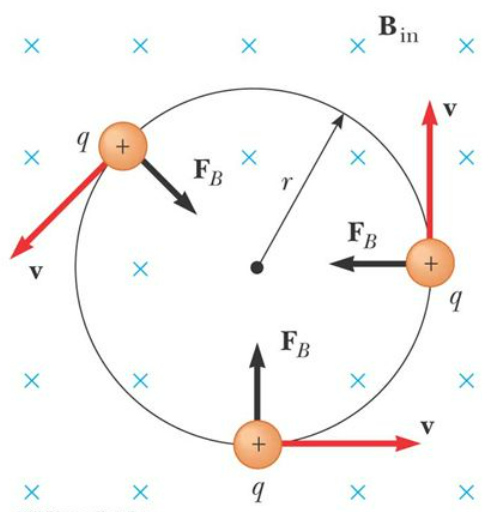
\includegraphics[width=8cm]{images/b_field_circularmotion.png}
\end{figure}

Period of revolution:
\[ T=\frac{2\pi r}{v} = \frac{2\pi\brac{\frac{mv}{Bq}}}{v} = \frac{2\pi m}{Bq} \] which is independent of $v$.

If $v$ and $B$ are not perpendicular, $0\degree < \theta < 90\degree$, charge moves in a helical path (i.e. it spirals forward).


\pagebreak

\subsubsection{Use of Crossed Fields}
Uniform $E$ and $B$ fields could be set up \underline{perpendicular} to each other such that they exert equal forces of opposite directions on a moving charged particle. This setup may be referred to as crossed fields.

A \textbf{velocity selector} emits a stream of charged particles (e.g. electrons) of a specific velocity.

\begin{figure}[H]
    \centering
    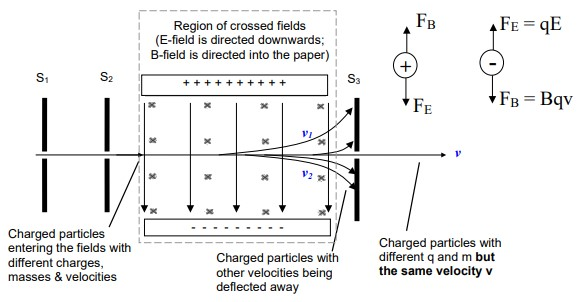
\includegraphics[width=14cm]{images/cross_fields.jpg}
\end{figure}

A beam of charged particles with a range of velocities $v_1,v_2,\dots,v_n$ pass through a region where there is a crossed field.

If the charged particles were electrons, then each electron in the crossed field experiences an upward electric force, and a downward magnetic force. (For positively charged particles: a downward electric force and an upward magnetic force)

For the particles to pass through undeflected, electric force and magnetic force are equal in magnitude:
\[ F_B = F_E \implies Bqv = qE \implies \boxed{v=\frac{E}{B}} \]
\pagebreak

\subsection*{Problems}


\pagebreak
\section{Electromagnetic Induction}
\textbf{Electromagnetic induction} is the phenomenon where an e.m.f. is induced due to a changing magnetic field.

\subsection{Magnetic flux}
\begin{defn}{Magnetic flux $\Phi$}{}
Product of the component of the magnetic field density normal to the plane of the surface and the area of the
surface.
\begin{equation}
\Phi = B_{\perp}A = BA\cos\theta
\end{equation}
where $\theta$ is the angle between the normal of the plane and the magnetic field.
\end{defn}

Unit of magnetic flux is the weber (Wb). \textbf{Weber} is the flux of a uniform magnetic field $B$ of flux density 1 \unit{T}, through a plane surface of area $A$ of 1 \unit{m^2}, placed normally to the $B$ field.

\begin{figure}[H]
    \centering
    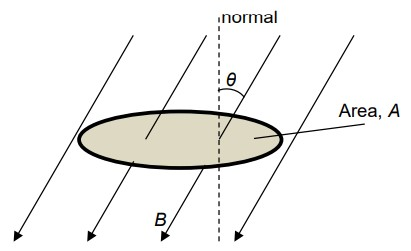
\includegraphics[width=8cm]{images/magnetic_flux.jpg}
\end{figure}

If area $A$ is bounded by a coil and the coil has $N$ turns, then the total magnetic flux passing through the coil (\textbf{magnetic flux linkage} through the coil) is
\begin{equation}
N\Phi = NBA\cos\theta
\end{equation}

From the equation, magnetic flux linkage through a coil depends on
\begin{itemize}
\item number of turns in coil $N$
\item magnitude of magnetic flux density $B$
\item surface area $A$
\item orientation of the coil $\theta$ with respect to the direction of $B$ ($\theta$ is the angle between the magnetic flux density and the normal of area of coil)
\end{itemize}

\begin{defn}{Magnetic flux linkage}{}
Product of magnetic flux passing through the coil and
number of turns on the coil.
\end{defn}
\pagebreak

\subsection{Laws of electromagnetic induction}
It was discovered experimentally that a changing magnetic field could induce an electric current in a circuit.

\begin{defn}{Faraday's law}{}
When the magnetic flux linkage with a circuit is changed, an induced e.m.f. is set up whose magnitude is directly proportional to rate of change of magnetic flux linkage.
\[ \varepsilon \propto \dv{(N\Phi)}{t} \]
\end{defn}

\begin{defn}{Lenz's law}{}
Induced e.m.f. (and hence current flow in a closed circuit)\footnote{A current is induced only if there is a complete circuit. An e.m.f. is always induced when there is a change in flux linkage.} is in a direction so as to produce effects which oppose the change that produces it.
\begin{equation}
\varepsilon = -\dv{(N\Phi)}{t} = -\dv{(NBA\cos\theta)}{t}
\end{equation}
\end{defn}

Lenz's Law is a consequence of the principle of conservation of energy.
\begin{itemize}
\item As the external agent brings the magnet towards the coil, by Lenz’s law, a current is induced in such a direction that the coil opposes, (i.e. repels) the approaching magnet.
\item Consequently, work has to be done by the external agent to overcome this opposition (the repulsive force).
\item It is this work done which is the source of the electrical energy.
\end{itemize}

\begin{tcolorbox}
\textbf{Fleming’s Right Hand rule}: determine direction of induced e.m.f. (and hence current in closed circuit).
\begin{itemize}
\item seCond finger represents Current
\item First finger represents magnetic Field
\item thumb represents force (or direction of motion)
\end{itemize}
\end{tcolorbox}

\subsubsection{Motional e.m.f. (Cutting of magnetic field)}
Motional e.m.f. is the e.m.f. induced in a conductor moving through a uniform magnetic field.

\begin{figure}[H]
    \centering
    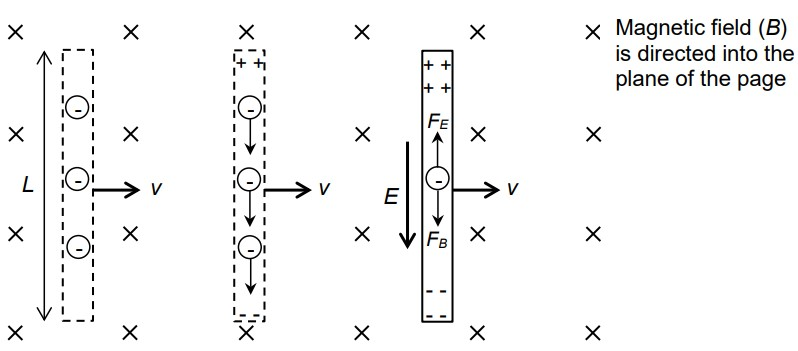
\includegraphics[width=12cm]{images/motional_emf.jpg}
\end{figure}

\begin{itemize}
\item When a conductor (wire) moves at a constant velocity in a uniform magnetic field, the moving conductor cuts magnetic field (or flux). An induced e.m.f. is generated when there is a cutting of flux. 
\item When the conductor is pushed to move to the right, free electrons in the conductor move to the right, so current flows to the left. Based on Fleming’s left-hand rule, each electron experiences downward magnetic force. 
\item Under the influence of this force, electrons move to the lower end of the conductor and accumulate there, leaving a net positive charge at the upper end. As a result of charge separation, electric field (directed downward) is produced inside the conductor. 
\item Charges accumulate at both ends until downward magnetic force is balanced by upward electric force.
\end{itemize}
\[ F_E = F_B \implies qE = qvB \implies E = vB \]

Since the electric field in the conductor is uniform, potential difference across the ends of conductor of length $L$ is given by $\Delta V=EL$ thus
\begin{equation}
\varepsilon = BLv
\end{equation}

Therefore an e.m.f. $\varepsilon$ is induced as long as the conductor continues to move through the uniform magnetic field. If the direction of the motion is reversed, polarity of induced e.m.f. is also reversed.

In summary, induced e.m.f. is also proportional to the rate of flux cutting.

For a moving conductor on a circuit with a resistance $R$ connected in series,
\[ \Delta V = BLv \implies \boxed{I=\frac{BLv}{R}} \]
\pagebreak

\subsection{Applications}
\subsubsection{Generator}
Electric generators take in energy by work and transfer it out by electrical transmission. 

\subsubsection{Eddy currents}
When a conductor is subjected to a changing magnetic flux, induced e.m.f. causes currents to flow. If the conductor is in the shape of a loop, induced current flows around the loop. However if the conductor is a solid plate, induced currents, known as \textbf{Eddy currents}, flow simultaneously along many different paths in swirls.

This can be demonstrated by allowing a flat copper or aluminium plate attached to the end of a rigid bar to swing back and forth through a magnetic field. As the plate enters the field, the plate cuts the magnetic field/flux. The changing magnetic flux induces an e.m.f. in the plate. The field in the plate is not uniform and the rate of cutting is not the same over the whole plate, so different e.m.f. are induced in different parts of plate, leading to eddy currents in the plate.

[figure]

As the swinging plate enters the field at position 1, the flux due to the external magnetic field into the page through the plate is increasing, hence by Lenz's law the induced eddy current must provide its own magnetic field out of the page. Direction of the induced current is thus anticlockwise. The opposite is true as the plate leaves the field at position 2, where the current is clockwise.

\paragraph{Applications}
set up a braking system which can rapidly change kinetic energy to other forms of energy. This can be taken a step further if a circuit can be built to channel the electrical energy from the kinetic energy back into the battery. This is what most hybrid cars do.

Stop rollercoasters, galvanometers, voltmeters and ammeters.

\paragraph{Drawbacks}
Eddy currents are dissipated as heating in the conductor (i.e. the conductor gets heated up).

Loss of energy in applications such as a transformer, as induced currents do work and raise the temperature of the iron core and cause energy loss.

Eddy currents can be reduced by eliminating paths for the current flow, for example, by cutting slits in the plate. These slits will prevent large eddy currents from occurring.
\pagebreak

\subsection*{Problems}

\pagebreak
\section{Alternating Current}
\begin{defn}{Alternating current (a.c.)}{}
Current that varies periodically with time in magnitude and direction. 

(Polarity of the voltage source constantly changes)
\end{defn}

\subsection{Characteristics}
\textbf{Period} $T$: time taken for the current to undergo one complete cycle.

\textbf{Frequency} $f$: number of complete cycles undergone by the current per unit time.

\textbf{Angular frequency} $\omega$: frequency in terms of radians per unit time rather than cycles per unit time.
\[ \omega = \frac{2\pi}{T} \]

\textbf{Peak value} $I_0$: maximum magnitude of the current attained in each cycle.

\textbf{Peak-to-peak value} $I_{pp}$: difference between the maximum and minimum values of the current within one cycle.

For a sinusoidal wave, 
\[ I_{pp} = 2I_0 \]

Mean Value $\langle I\rangle$: average value of a.c. over a given time interval.

Root mean square value $I_\text{r.m.s.}$: value of alternating current that is equal to the steady direct current which would dissipate heat at the same average rate in a given resistor.

The most commonly encountered form of a.c. is the \textbf{sinusoidal} form, that is, it varies with time according to a sine or cosine function.

\begin{equation}
I = I_0 \sin \omega t
\end{equation}

Similarly, potential difference across the resistor is given by 
\[ V = V_0 \sin \omega t \]



\subsection{Transformer}
\subsubsection{Functioning}

\subsubsection{Turns ratio}

\subsubsection{Power loss}
Practical transformers lose power through
\begin{itemize}
\item \textbf{Joule heating}

The wires used for the windings of the coils have resistance and so heating occurs, resulting in power loss $P=I^2R$. Thicker wires made of material with low resistivity (i.e. high purity copper) are used to reduce this power loss.

\item \textbf{Eddy currents}

The alternating magnetic flux induces eddy currents in the iron core and cause heating. This effect is reduced by laminating the iron core. Laminations reduce the area of circuits in the core, and thus reduce the e.m.f. induced and current flowing within the core, which leads to a reduction in the energy lost.

\item \textbf{Hysteresis loss}

Magnetisation of the core is repeatedly reversed by the alternating magnetic field. The energy required to magnetise the core (while the current is increasing) is not entirely recovered during demagnetisation. The difference in energy is lost as heat in the core. The energy loss is kept to a minimum by using a magnetic material with low hysteresis loss.

\item \textbf{Flux leakage}

The flux due to the primary may not all link to the secondary coil if the coil is badly designed or has air gaps in it. When flux is “leaked “to the surrounding, power is loss and thus not all the power from the primary coil can be transferred to the secondary coil.
\end{itemize}


\subsection{Rectification with a diode}

\pagebreak

\subsection*{Problems}

\pagebreak

\part{Modern Physics}
\section{Quantum Physics}
\subsection{Photoelectric effect}
\begin{defn}{Photoelectric effect}{}
Emission of electrons from metal surface when electromagnetic radiation of sufficiently high frequency is incident on it.
\end{defn}

Experimental observations from the photoelectric effect experiment:
\begin{enumerate}
\item No electrons are emitted if the frequency of the EM radiation is below a minimum frequency (called the threshold frequency $f_0$), regardless of the intensity of the radiation.
\item Photoelectric current is proportional to the intensity of radiation, for a fixed frequency (because the rate of emission of electrons $\propto$ rate of incidence of photons)
\item Max KE of photo-electrons depends only on the frequency and the work function $\phi$ of the metal used, not the intensity. (Note: Emitted electrons have a range of kinetic energy, ranging from zero to a certain maximum value.)
\item Emission of electrons begins instantaneously (i.e. no (measurable) time lag between emission and illumination) even if the intensity is low.
\end{enumerate}

(1), (2) and (3) cannot be explained by Classical Wave Theory of Light; they provide evidence for the particulate\footnote{particle-like} nature of EM radiation.

Failure of the classical wave theory to explain the photoelectric effect
\begin{itemize}
\item According to the “Particle Theory of Light”, EM radiation consists of a stream of particles/ photons/ discrete energy packets, each of energy hf.
\item An electron is ejected when a single photon of sufficiently high frequency, transfers ALL its energy in a discrete packet to the electron.
\item According to equation, $hf - \phi = \frac{1}{2}m_ev^2$, if the energy of the photon hf < the minimum energy required for emission ($\phi$), no emission can take place, no matter how intense the light may be. {Explains observation (1)}
\item This also explains why, (even at very low intensities), as long as $hf > \phi$, emission takes place without a time delay between illumination of the metal and ejection of electrons. {Explains observation(4)}
\end{itemize}

\subsection{Energy of a photon}
Particulate nature of electromagnetic radiation:
\begin{itemize}
\item Electromagnetic radiation can be said to be particulate in nature in addition to being waved in nature.
\item A beam of light consists of small discrete quanta of electromagnetic energy known as photons.
\item Photons transfer either all or none of their energy to another particle instantaneously, contrary to the wave theory which states that the energy transfer is continuous.
\end{itemize}

\begin{defn}{Photon}{}
A discrete packet (or quantum) of energy of an electromagnetic radiation with energy $hf$.
\end{defn}

Energy of a photon is given by
\begin{equation}
E = \hbar f
\end{equation}
where \textbf{Planck constant} $\hbar = 6.63 \times 10^{-34}\unit{J}\unit{s}$.



\subsection{Wave-particle duality}
Waves can exhibit particle-like characteristics and particles can exhibit wave-like characteristics.

de Broglie wavelength of a particle: 
\begin{equation}
\lambda = \frac{h}{p}
\end{equation}

Packets of EM radiation of wavelength $\lambda$ would therefore possess a momentum $p=\frac{h}{\lambda}$. When photons are incident on a surface, they therefore exert a force on the surface, resulting in a pressure on the surface. This pressure is known as “radiation pressure”. 

Using $KE=\frac{p^2}{2m}$,  wavelength of a particle
can be related to its KE by
\begin{equation}
\lambda = \frac{h}{\sqrt{2m(KE)}}
\end{equation}

\subsection{Energy levels in atoms}


\subsection{Line spectra}


\subsection{X-ray spectra}


\subsection{Uncertainty principle}
\begin{defn}{Heisenberg position-momentum uncertainty principle}{}
It is impossible to measure the exact position and momentum of a body at the same time. It can be expressed as
\begin{equation}
\Delta p \Delta x \ge \hbar
\end{equation}
where $\Delta p$ and $\Delta x$ denote the uncertainties in the momentum and position of the particle respectively.
\end{defn}

\subsection*{Problems}

\pagebreak
\section{Nuclear Physics}
\subsection{The nucleus}


\subsection{Isotopes}


\subsection{Nuclear processes}


\subsection{Mass defect and nuclear binding energy}


\subsection{Radioactive decay}


\subsection{Biological effects of radiation}


\subsection*{Problems}

\pagebreak

\appendix
\section{Derivations}\label{appendix}
\subsection{Kinematics}
\textbf{Equations of motion}
\[ v=u+at \]
\begin{proof}[Derivation]
This is from the definition of acceleration.
\end{proof}

\[ s=\frac{1}{2}(u+v)t \]
\begin{proof}[Derivation]
Computing the area under a velocity-time graph (which has the shape of a trapezoid) gives the displacement.
\end{proof}

\[ s=ut+\frac{1}{2}at^2 \]
\begin{proof}[Derivation]
Substitute \cref{eqn_mtn1} into \cref{eqn_mtn2} to remove $v$.
\end{proof}

\[ v^2=u^2+2as \]
\begin{proof}[Derivation]
Rewrite \cref{eqn_mtn1} to give $t=\dfrac{v-u}{a}$ which we can substitute into \cref{eqn_mtn2} to remove $t$.
\end{proof}
\pagebreak

\subsection{Forces}
\textbf{Spring constant}

For springs in parallel, 
\[ k_{\text{eff}} = \sum_{i} k_i \]

\begin{proof}[Derivation]
Extension of all springs is the same, total force is the sum of forces acting on all springs.
\[ F = \sum_{i} F_i \implies k_{\text{eff}} x = \sum_{i} F_i x \implies k_{\text{eff}} = \sum_{i} k_i \]
\end{proof}

For springs in series,
\[ \frac{1}{k_{\text{eff}}} = \sum_{i} \frac{1}{k_i} \]

\begin{proof}[Derivation] Force acting on all springs is the same, total extension is the sum of extensions of all springs.
\[ x = \sum_{i} x_i \implies \frac{F}{k_{\text{eff}}} = \sum_{i} \frac{F}{k_i} \implies \frac{1}{k_{\text{eff}}} = \sum_{i} \frac{1}{k_i} \]
\end{proof}

\textbf{Pressure}
\[ P=\rho g h \]

\begin{proof}[Derivation]
Given a liquid column of height $h$ and cross-sectional area $A$, of density $rho$.
\[ m = \rho V = (Ah)\rho\]
Weight $W$ of the liquid column above $A$ is 
\[ W = mg = \rho Vg = Ah\rho g \]
Hence pressure on area $A$ is given by
\[ \rho = \frac{F}{A} = \frac{Ah\rho g}{A} = \rho g h \]
\end{proof}

\textbf{Upthrust}
\[ U=W_{\text{displaced}} \]

\begin{proof}[Derivation]
Consider a solid cylinder of height $h$ and cross-sectional area $A$, submerged in a liquid of density $\rho$.

Pressure on the top surface is given by 
\[ p_1 = \rho g h_1 + p_0 \]
Hence downward force on top surface is 
\[ F_1 = (\rho g h_1 + p_0)A \]

Similarly, pressure on the bottom surface is given by 
\[ p_2 = \rho g h_2 + p_0 \]

Upward force on bottom surface is 
\[ F_2 = (\rho g h_2 + p_0)A \]

Hence, the resultant upward force (upthrust) on the cylinder is 
\begin{align*}
U &= F_2 - F_1 \\
&= \rho g (h_2 - h_1) A \\
&= \rho g h A \\
&= \rho g V_{\text{displaced}} \\
&= m_{\text{displaced}} g
\end{align*}
which is equal to the weight of fluid displaced by the object.
\end{proof}
\pagebreak

\subsection{Work, Energy, Power}
\textbf{Work done by gas}
\[ W = p \Delta V \]

\begin{proof}[Derivation]
Consider gas at pressure $p$ in a syringe which has a frictionless piston of cross-sectional area $A$, then the force exerted by gas on piston is $F=pA$. If the gas expands slowly (pressure of gas remains constant) against a constant external pressure moving outwards a displacement $s$, then force $F$ is constant.

Work done by gas in expanding from $V_1$ to $V_2$ is given by
\[ W = Fs = (pA)s = p(As) = p \Delta V = p (V_2 - V_1) \]

When the gas expands ($V_2>V_1$), work done by gas is positive.

When the gas expands ($V_2<V_1$), work done by gas is negative.
\end{proof}

\textbf{Gravitational potential energy}
\[ \mathrm{GPE} = mgh \]

\begin{proof}[Derivation]
Consider an object being raised from height $h_1$ to height $h_2$ by a constant force $F$ equal and opposite to the weight $mg$ of the object (so that object does not gain KE).
\[ F=mg \]

Work done by force $F$ changes gravitational potential energy, is given by
\begin{align*}
    W &= F \Delta h \\
    &= F (h_2 - h_1) \\
    &= mg (h_2 - h_1) \\
    &= mgh_2 - mgh_1 \\
    &= \mathrm{GPE}_f - \mathrm{GPE}_i
\end{align*}

Therefore, gravitational potential energy is $\mathrm{GPE} = mgh$.
\end{proof}

\textbf{Kinetic energy}
\[ \mathrm{KE} = \frac{1}{2}mv^2 \]

\begin{proof}[Derivation]
Consider a stationary body of mass $m$ which moves a horizontal displacement $s$ under the action of a constant net force $F$. Since the force is constant, body moves with constant acceleration $a$. 

By Newton's 2nd Law of Motion,
\[ F = ma \]

The final velocity $v$ of the body is given by 
\[ v^2 = u^2 + 2as \implies v^2 = 2as \implies s = \frac{v^2}{2a} \]

Hence, work done on the body is 
\[ W = Fs = ma \brac{\frac{v^2}{2a}} = \frac{1}{2}mv^2 \]

Work done by force $F$ increases the kinetic energy of the body. 

Therefore, the kinetic energy of a body at speed $v$ is $\mathrm{KE} = \dfrac{1}{2}mv^2$.
\end{proof}

\textbf{Instantaneous power}
\[ P = Fv \]

\begin{proof}[Derivation]
\[ P = \dv{W}{t} = \dv{(Fs)}{t} = F\dv{s}{t} = Fv \]
\end{proof}
\pagebreak

\subsection{Circular motion}
\begin{equation} a = \frac{v^2}{r} = r\omega^2 \end{equation}

\begin{proof}[Derivation]
The two velocity vectors $v_1$ and $v_2$ can be rearranged to form a triangle which is similar to the triangle formed by the radii $r_1$, $r_2$ and displacement $s$.
\begin{figure}[H]
	\centering
	\includegraphics[width=12cm]{Centripetal_acceleration}
\end{figure}
Using similar triangles,
\[ \frac{\Delta s}{r} = \frac{\Delta v}{v} \implies \frac{\Delta s}{\Delta t}\cdot\frac{1}{r} = \frac{\Delta v}{\Delta t}\cdot\frac{1}{v} \]
Taking limits where $\Delta t \to 0$,
\[ \frac{1}{r}\brac{\lim_{\Delta t \to 0}\frac{\Delta s}{\Delta t}} = \frac{1}{v}\brac{\lim_{\Delta t \to 0}\frac{\Delta v}{\Delta t}} \implies \frac{1}{r}\dv{s}{t}=\frac{1}{v}\dv{v}{t} \implies \frac{v}{r} = \frac{a}{v} \implies a = \frac{v^2}{r} \]
\end{proof}
\pagebreak

\subsection{Gravitational Field}
\textbf{Gravitational field strength}
\[ g=-\frac{GM}{r^2} \]
\begin{proof}[Derivation]
Newton's Law of Gravitation states that 
\[ F=-\frac{GMm}{r^2} \]
By the definition of gravitational field strength,
\[ g=\frac{F}{m}=\frac{-\frac{GMm}{r^2}}{m}=-\frac{GM}{r^2} \]
\end{proof}

\textbf{Gravitational field strength near the surface}
\begin{proof}[Derivation]
Consider gravitational field strength at height $h$ above the surface of Earth. Near the surface of Earth, $h$ is small compared to the radius $R$ of Earth, i.e. $h \ll R$.
\[ g = \frac{GM}{(h+R)^2} \approx \frac{GM}{R^2} \]
\end{proof}

\textbf{Gravitational potential energy}
\[ U = -\frac{GMm}{r} \]

\begin{proof}[Derivation]
Consider moving a mass $m$ from infinity to a point at distance $r$ from a mass $M$ at \emph{constant speed} (so that kinetic energy of mass $m$ does not change).

From the definition of gravitational potential energy,
\[ U = \int_{\infty}^r \va{F}_{\mathrm{ext}} \dd{r} \]
Since the external force acts in the opposite direction of gravitational force, $\va{F}_{\mathrm{ext}}=-\va{F}_g$.
\[ U = \int_{\infty}^r -\va{F}_g \dd{r} = \int_{\infty}^r \frac{GMm}{r^2} \dd{r} \]
Computing the integral, 
\[ U = \sqbrac{-\frac{GMm}{r}}^r_{\infty} = -\frac{GMm}{r} \]
\end{proof}
\pagebreak

\subsection{Temperature and Ideal Gases}
\textbf{Kinetic theory of gas}
\[ pV = \frac{1}{3} Nm \langle c^2 \rangle \]
\begin{proof}[Derivation]
Consider an ideal gas consisting of $N$ identical molecules, each of mass $m$, in a cubical container of side length $L$.

Since the molecules move randomly, they do not have any preferred direction of travel along the $x$-, $y$- and $z$-axes. We expect that one-third of the $N$ molecules move along each axis.

Consider a one-dimensional case along the $x$-axis. One gas molecule of mass $m$ approaches and collides elastically with the wall with velocity $c_x$, and leaves the wall with velocity $-c_x$. Change in momentum of gas molecule is given by 
\[ \Delta p = -2mc_x \]

By conservation of linear momentum, wall experiences change in momentum of
\[ \Delta p_\text{wall} = 2mc_x \]

After the collision, assume this molecule continues its motion uninterrupted. It travels a total distance of $2L$ back and forth, and collides with the same wall. The time interval between successive collisions is given by 
\[ \Delta t = \frac{2L}{c_x} \]

Rate of change of momentum of wall due to one molecule is given by 
\[ \frac{\Delta p_\text{wall}}{\Delta t} = -\frac{m{c_x}^2}{L} \]

By Newton's 2nd law, net force on wall is rate of change of momentum of wall due to all $N$ molecules, given by
\begin{align*}
F_\text{wall} &= \frac{m{c_{x1}}^2}{L} + \cdots + \frac{m{c_{xN}}^2}{L} \\
&= \frac{m}{L}\brac{{c_{x1}}^2 + \cdots + {c_{xN}}^2} \\
&= \frac{Nm}{L}\langle {c_x}^2 \rangle
\end{align*}
where mean square speed $\langle {c_x}^2 \rangle$ is defined as
\[ \langle {c_x}^2 \rangle = \frac{{c_{x1}}^2 + \cdots + {c_{xN}}^2}{N} \]

Since the area of the wall is $L^2$, pressure on wall is given by 
\begin{equation*}\tag{1}
p = \frac{F}{L^2} = \frac{Nm}{V}\langle {c_x}^2 \rangle
\end{equation*}
since $V=L^3$.

Applying Pythagoras' Theorem to 3D velocity vector of molecule gives
\[ c^2={c_x}^2+{c_y}^2+{c_z}^2 \implies \langle c^2 \rangle = \langle {c_x}^2 \rangle + \langle {c_y}^2 \rangle + \langle {c_z}^2 \rangle \]

Since there are $\dfrac{N}{3}$ molecules moving along each axis, $\langle {c_x}^2 \rangle = \langle {c_y}^2 \rangle = \langle {c_z}^2 \rangle$. Hence
\[ \langle {c_x}^2 \rangle = \frac{1}{3}\langle c^2 \rangle \]
Substituting this into (1) gives us
\[ pV = \frac{1}{3} Nm \langle c^2 \rangle \]
as desired.
\end{proof}
\begin{remark}
How to remember the derivation:
\begin{itemize}
\item Context, find pressure $P=\frac{F}{A}$
\item Origin of force $F$: collision of one, $N$ gas molecules with wall. Relate rate of change of $\delta p$ to $F=\dv{p}{t}$
\item Generalise for $N$ molecules, apply mean square speed
\end{itemize}
\end{remark}
\begin{remark}
The root mean square is an estimation of a statistical ``average''. Statistically, the \textbf{root mean squared speed} of gas molecules means taking the square root of the sum of the squares of the speeds of all gas molecules.
\[ c_{\text{r.m.s.}} = \sqrt{\frac{{c_1}^2+{c_2}^2+\cdots+{c_n}^2}{n}} \]
\end{remark}
\pagebreak

\subsection{Oscillations}
\textbf{Velocity}
\[ v=\pm\omega\sqrt{{x_0}^2-x^2} \]
\begin{proof}[Derivation]
Displacement is given by
\[ x=x_0\sin\omega t \]
By differentiation, velocity is given by
\[ v=\omega x_0\cos\omega t \]
Using Pythagorean identity $\sin^2 x+\cos^2 x=1$, the given equation can be easily derived.
\end{proof}
\pagebreak

\subsection{Wave Motion}
\textbf{Wave speed}
\[ v=f\lambda \]
\begin{proof}[Derivation]
One wavelength $\lambda$ is distance travelled by wave during one complete oscillation of the source.

Distance travelled by wave during $n$ complete oscillations is $n\lambda$.

Speed of wave is distance per unit time, $v=\dfrac{n\lambda}{t}$.

Frequency is number of oscillations per unit time, $f=\dfrac{n}{t}$.

Hence
\[ f\lambda=\brac{\frac{n}{t}}\lambda=\frac{n\lambda}{t}=v. \]
\end{proof}
\pagebreak

\subsection{Current of Electricity}
\textbf{Transport equation}
\[ I=nAvq \]

\begin{proof}[Derivation]
Consider a current $I$ passing through a section of a wire of cross-sectional area $A$. 

We define
\begin{itemize}
\item $n$ as number density of charge carriers (number per unit volume)
\item $q$ as amount of charge of each charge carrier
\item $v$ as drift velocity of charge carriers
\end{itemize}
\[ I=\frac{Q}{t}=\frac{Nq}{t}=\frac{nVq}{t}=\frac{nAxq}{t}=nAvq \]
\end{proof}
\pagebreak

\section{Summary of Key Quantities, Symbols and Units}
\renewcommand*{\arraystretch}{1.4}
\begin{longtable}[H]{p{0.60\textwidth} p{0.15\textwidth} p{0.15\textwidth}}
\toprule
\textbf{Quantity} & \textbf{Symbol} & \textbf{Unit} \\
\midrule
\endhead
Displacement (or equivalent) & $s$, $x$ & $\unit{m}$ \\*
Velocity & $v$ & $\unit{m.s^{-1}}$ \\*
Acceleration & $a$ & $\unit{m.s^{-2}}$ \\*
\midrule
Force & $F$ & $\unit{N}$ \\*
Weight & $W$ & $\unit{N}$ \\*
Normal force & $N$ & $\unit{N}$ \\*
Tension & $T$ & $\unit{N}$ \\*
Friction & $f$ & $\unit{N}$ \\*
Upthrust & $U$ & $\unit{N}$ \\*
Moment & $M$ & $\unit{N.m}$ \\*
Work done & $W$ & $\unit{J}$ \\*
Energy & $E$ & $\unit{J}$ \\*
Power & $P$ & $\unit{W}$ \\*
Efficiency & $\eta$ & \\*
\midrule
Angular displacement & $\theta$ & $\unit{rad}$ \\*
Angular velocity & $\omega$ & $\unit{rad.s^{-1}}$ \\*
Centripetal acceleration & $a$ & $\unit{m.s^{-2}}$ \\*
Centripetal force & $F_c$ & $\unit{N}$ \\*
Period & $T$ & $\unit{s}$ \\*
Frequency & $f$ & $\unit{Hz}$ \\*
\midrule
Gravitational force & $F_g$ & $\unit{N}$ \\*
Gravitational field strength & $g$ & $\unit{N.kg^{-1}}$ \\*
Gravitational potential energy & $U$ & $\unit{J}$ \\*
Gravitational potential & $\phi$ & $\unit{J.kg^{-1}}$ \\*
\midrule
Pressure & $p$ & \unit{Pa} \\*
Volume & $V$ & \unit{m^3} \\*
Moles (amount) & $n$ & \unit{mol} \\*
Temperature & $T$ & \unit{K} \\*
Number of gas particles & $N$ & -- \\*
Mass of gas & $M$ & \unit{kg} \\*
Molar mass & $M_r$ & \unit{g.mol^{-1}} \\*
Molar volume & $V_m$ & \unit{m^3} \\*
\midrule
Amplitude & $x_0$ & $\unit{m}$ \\*
Angular frequency & $\omega$ & $\unit{rad.s^{-1}}$ \\*
Phase & $\omega t+\phi$ & $\unit{rad}$ \\*
Phase difference & $\phi$ & $\unit{rad}$ \\*
\midrule
Current & $I$ & $A$ \\*
Potential difference & $V$ & $V$ \\*
Electromotive force & $\epsilon$ & $V$ \\*
Resistance & $R$ & $\Omega$ \\*
Resistivity & $\rho$ & $\unit{\Omega.m}$ \\*
\midrule
\end{longtable}

\end{document}